% Options for packages loaded elsewhere
\PassOptionsToPackage{unicode}{hyperref}
\PassOptionsToPackage{hyphens}{url}
\PassOptionsToPackage{dvipsnames,svgnames,x11names}{xcolor}
%
\documentclass[
  letterpaper,
  DIV=11,
  numbers=noendperiod]{scrreprt}

\usepackage{amsmath,amssymb}
\usepackage{iftex}
\ifPDFTeX
  \usepackage[T1]{fontenc}
  \usepackage[utf8]{inputenc}
  \usepackage{textcomp} % provide euro and other symbols
\else % if luatex or xetex
  \usepackage{unicode-math}
  \defaultfontfeatures{Scale=MatchLowercase}
  \defaultfontfeatures[\rmfamily]{Ligatures=TeX,Scale=1}
\fi
\usepackage{lmodern}
\ifPDFTeX\else  
    % xetex/luatex font selection
\fi
% Use upquote if available, for straight quotes in verbatim environments
\IfFileExists{upquote.sty}{\usepackage{upquote}}{}
\IfFileExists{microtype.sty}{% use microtype if available
  \usepackage[]{microtype}
  \UseMicrotypeSet[protrusion]{basicmath} % disable protrusion for tt fonts
}{}
\makeatletter
\@ifundefined{KOMAClassName}{% if non-KOMA class
  \IfFileExists{parskip.sty}{%
    \usepackage{parskip}
  }{% else
    \setlength{\parindent}{0pt}
    \setlength{\parskip}{6pt plus 2pt minus 1pt}}
}{% if KOMA class
  \KOMAoptions{parskip=half}}
\makeatother
\usepackage{xcolor}
\setlength{\emergencystretch}{3em} % prevent overfull lines
\setcounter{secnumdepth}{5}
% Make \paragraph and \subparagraph free-standing
\makeatletter
\ifx\paragraph\undefined\else
  \let\oldparagraph\paragraph
  \renewcommand{\paragraph}{
    \@ifstar
      \xxxParagraphStar
      \xxxParagraphNoStar
  }
  \newcommand{\xxxParagraphStar}[1]{\oldparagraph*{#1}\mbox{}}
  \newcommand{\xxxParagraphNoStar}[1]{\oldparagraph{#1}\mbox{}}
\fi
\ifx\subparagraph\undefined\else
  \let\oldsubparagraph\subparagraph
  \renewcommand{\subparagraph}{
    \@ifstar
      \xxxSubParagraphStar
      \xxxSubParagraphNoStar
  }
  \newcommand{\xxxSubParagraphStar}[1]{\oldsubparagraph*{#1}\mbox{}}
  \newcommand{\xxxSubParagraphNoStar}[1]{\oldsubparagraph{#1}\mbox{}}
\fi
\makeatother


\providecommand{\tightlist}{%
  \setlength{\itemsep}{0pt}\setlength{\parskip}{0pt}}\usepackage{longtable,booktabs,array}
\usepackage{calc} % for calculating minipage widths
% Correct order of tables after \paragraph or \subparagraph
\usepackage{etoolbox}
\makeatletter
\patchcmd\longtable{\par}{\if@noskipsec\mbox{}\fi\par}{}{}
\makeatother
% Allow footnotes in longtable head/foot
\IfFileExists{footnotehyper.sty}{\usepackage{footnotehyper}}{\usepackage{footnote}}
\makesavenoteenv{longtable}
\usepackage{graphicx}
\makeatletter
\newsavebox\pandoc@box
\newcommand*\pandocbounded[1]{% scales image to fit in text height/width
  \sbox\pandoc@box{#1}%
  \Gscale@div\@tempa{\textheight}{\dimexpr\ht\pandoc@box+\dp\pandoc@box\relax}%
  \Gscale@div\@tempb{\linewidth}{\wd\pandoc@box}%
  \ifdim\@tempb\p@<\@tempa\p@\let\@tempa\@tempb\fi% select the smaller of both
  \ifdim\@tempa\p@<\p@\scalebox{\@tempa}{\usebox\pandoc@box}%
  \else\usebox{\pandoc@box}%
  \fi%
}
% Set default figure placement to htbp
\def\fps@figure{htbp}
\makeatother

\KOMAoption{captions}{tableheading}
\makeatletter
\@ifpackageloaded{bookmark}{}{\usepackage{bookmark}}
\makeatother
\makeatletter
\@ifpackageloaded{caption}{}{\usepackage{caption}}
\AtBeginDocument{%
\ifdefined\contentsname
  \renewcommand*\contentsname{Table of contents}
\else
  \newcommand\contentsname{Table of contents}
\fi
\ifdefined\listfigurename
  \renewcommand*\listfigurename{List of Figures}
\else
  \newcommand\listfigurename{List of Figures}
\fi
\ifdefined\listtablename
  \renewcommand*\listtablename{List of Tables}
\else
  \newcommand\listtablename{List of Tables}
\fi
\ifdefined\figurename
  \renewcommand*\figurename{Figure}
\else
  \newcommand\figurename{Figure}
\fi
\ifdefined\tablename
  \renewcommand*\tablename{Table}
\else
  \newcommand\tablename{Table}
\fi
}
\@ifpackageloaded{float}{}{\usepackage{float}}
\floatstyle{ruled}
\@ifundefined{c@chapter}{\newfloat{codelisting}{h}{lop}}{\newfloat{codelisting}{h}{lop}[chapter]}
\floatname{codelisting}{Listing}
\newcommand*\listoflistings{\listof{codelisting}{List of Listings}}
\usepackage{amsthm}
\theoremstyle{plain}
\newtheorem{proposition}{Proposition}[chapter]
\theoremstyle{remark}
\AtBeginDocument{\renewcommand*{\proofname}{Proof}}
\newtheorem*{remark}{Remark}
\newtheorem*{solution}{Solution}
\newtheorem{refremark}{Remark}[chapter]
\newtheorem{refsolution}{Solution}[chapter]
\makeatother
\makeatletter
\makeatother
\makeatletter
\@ifpackageloaded{caption}{}{\usepackage{caption}}
\@ifpackageloaded{subcaption}{}{\usepackage{subcaption}}
\makeatother

\usepackage{bookmark}

\IfFileExists{xurl.sty}{\usepackage{xurl}}{} % add URL line breaks if available
\urlstyle{same} % disable monospaced font for URLs
\hypersetup{
  pdftitle={MA4J1 Continuum Mechanics Notes},
  pdfauthor={Thomas Hudson},
  colorlinks=true,
  linkcolor={blue},
  filecolor={Maroon},
  citecolor={Blue},
  urlcolor={Blue},
  pdfcreator={LaTeX via pandoc}}


\title{MA4J1 Continuum Mechanics Notes}
\author{Thomas Hudson}
\date{2025-01-01}

\begin{document}
\maketitle

\renewcommand*\contentsname{Table of contents}
{
\hypersetup{linkcolor=}
\setcounter{tocdepth}{2}
\tableofcontents
}

\bookmarksetup{startatroot}

\chapter*{Preface}\label{preface}
\addcontentsline{toc}{chapter}{Preface}

\markboth{Preface}{Preface}

\newcommand{\bfa}{{\boldsymbol{a}}}
\newcommand{\bfb}{{\boldsymbol{b}}}
\newcommand{\bfc}{{\boldsymbol{c}}}
\newcommand{\bfd}{{\boldsymbol{d}}}
\newcommand{\bfe}{{\boldsymbol{e}}}
\newcommand{\bff}{{\boldsymbol{f}}}
\newcommand{\bfg}{{\boldsymbol{g}}}
\newcommand{\bfh}{{\boldsymbol{h}}}
\newcommand{\bfi}{{\boldsymbol{i}}}
\newcommand{\bfj}{{\boldsymbol{j}}}
\newcommand{\bfk}{{\boldsymbol{k}}}
\newcommand{\bfl}{{\boldsymbol{l}}}
\newcommand{\bfm}{{\boldsymbol{m}}}
\newcommand{\bfn}{{\boldsymbol{n}}}
\newcommand{\bfo}{{\boldsymbol{o}}}
\newcommand{\bfp}{{\boldsymbol{p}}}
\newcommand{\bfq}{{\boldsymbol{q}}}
\newcommand{\bfr}{{\boldsymbol{r}}}
\newcommand{\bfs}{{\boldsymbol{s}}}
\newcommand{\bft}{{\boldsymbol{t}}}
\newcommand{\bfu}{{\boldsymbol{u}}}
\newcommand{\bfv}{{\boldsymbol{v}}}
\newcommand{\bfw}{{\boldsymbol{w}}}
\newcommand{\bfx}{{\boldsymbol{x}}}
\newcommand{\bfy}{{\boldsymbol{y}}}
\newcommand{\bfz}{{\boldsymbol{z}}}

\newcommand{\bfA}{{\boldsymbol{A}}}
\newcommand{\bfB}{{\boldsymbol{B}}}
\newcommand{\bfC}{{\boldsymbol{C}}}
\newcommand{\bfD}{{\boldsymbol{D}}}
\newcommand{\bfE}{{\boldsymbol{E}}}
\newcommand{\bfF}{{\boldsymbol{F}}}
\newcommand{\bfG}{{\boldsymbol{G}}}
\newcommand{\bfH}{{\boldsymbol{H}}}
\newcommand{\bfI}{{\boldsymbol{I}}}
\newcommand{\bfJ}{{\boldsymbol{J}}}
\newcommand{\bfK}{{\boldsymbol{K}}}
\newcommand{\bfL}{{\boldsymbol{L}}}
\newcommand{\bfM}{{\boldsymbol{M}}}
\newcommand{\bfN}{{\boldsymbol{N}}}
\newcommand{\bfO}{{\boldsymbol{O}}}
\newcommand{\bfP}{{\boldsymbol{P}}}
\newcommand{\bfQ}{{\boldsymbol{Q}}}
\newcommand{\bfR}{{\boldsymbol{R}}}
\newcommand{\bfS}{{\boldsymbol{S}}}
\newcommand{\bfT}{{\boldsymbol{T}}}
\newcommand{\bfU}{{\boldsymbol{U}}}
\newcommand{\bfV}{{\boldsymbol{V}}}
\newcommand{\bfW}{{\boldsymbol{W}}}
\newcommand{\bfX}{{\boldsymbol{X}}}
\newcommand{\bfY}{{\boldsymbol{Y}}}
\newcommand{\bfZ}{{\boldsymbol{Z}}}

\newcommand{\bftau}{{\boldsymbol{\tau}}}
\newcommand{\bfnu}{{\boldsymbol{\nu}}}
\newcommand{\bfpsi}{{\boldsymbol{\psi}}}
\newcommand{\bfphi}{{\boldsymbol{\varphi}}}
\newcommand{\bfSigma}{{\boldsymbol{\Sigma}}}
\newcommand{\calI}{{\mathcal{I}}}
\newcommand{\calN}{{\mathcal{N}}}
\newcommand{\calV}{{\mathcal{V}}}
\newcommand{\bbE}{{\mathbb{E}}}
\newcommand{\bbR}{{\mathbb{R}}}
\newcommand{\bbC}{{\mathbb{C}}}
\newcommand{\bsfC}{{\mathsf{C}}}
\newcommand{\bsfD}{{\mathsf{D}}}
\newcommand{\bsfI}{{\mathsf{I}}}
\newcommand{\bsfO}{{\mathsf{O}}}
\newcommand{\tr}{{\operatorname{tr}}}
\newcommand{\sym}{{\operatorname{sym}}}
\newcommand{\skw}{{\operatorname{skew}}}
\newcommand{\vc}{{\operatorname{vec}}}
\newcommand{\ten}{{\operatorname{ten}}}
\newcommand{\cof}{{\operatorname{cof}}}
\newcommand{\mass}{{\operatorname{mass}}}
\newcommand{\vol}{{\operatorname{vol}}}
\newcommand{\area}{{\operatorname{area}}}
\newcommand{\com}{{\operatorname{com}}}
\newcommand{\cov}{{\operatorname{cov}}}
\newcommand{\e}{{\mathrm{e}}}
\newcommand{\D}{{\mathrm{D}}}
\newcommand{\dd}{{\mathrm{d}}}
\newcommand{\dt}{{\dd t}}
\newcommand{\Dt}{{\D t}}
\newcommand{\bigO}{{O}}
\newcommand{\litO}{{o}}
\newcommand{\dVx}{{\,\d V_{\bfx}}}
\newcommand{\dAx}{{\,\d A_{\bfx}}}
\newcommand{\dVy}{{\,\d V_{\bfy}}}
\newcommand{\dAy}{{\,\d A_{\bfy}}}
\newcommand{\ds}{{\,\d s}}

These notes are a guide to the main content of the fourth-year Maths
module MA4J1 Continuum Mechanics taught at Warwick. They are intended to
be essentially self--contained, but are based upon (my interpretation
of) the content of chapters drawn from
\href{https://go.exlibris.link/CMjyhLvJ}{A First Course in Continuum
Mechanics} by Oscar Gonzalez and Andrew Stuart. This book is a good
place to read more about the topics covered and to find various
exercises to test your understanding of the content, but it is
definitely not the only good book covering many of the topics we
consider here. In particular, for those looking for additional reading,
various additional books are recommended on the module Moodle page.

\section*{Aims and structure}\label{aims-and-structure}
\addcontentsline{toc}{section}{Aims and structure}

\markright{Aims and structure}

The central aim of the module is to present a mathematical framework
within which various continuum models of solids, liquids and gases can
be described and derived, and to provide some examples of the Partial
Differential Equation (PDE) models which result.

As background, we make use of various concepts from Linear Algebra,
Analysis and Vector Calculus. In Chapters @ref(cha:tensor-algebra) and
@ref(cha:tensor-calculus), we therefore recap various concepts and
discuss some operations on these objects which may be new to you, and at
the very least, may take a different perspective. Since some of these
concepts will be taken as understood, it will be up to you to ensure
that you are comfortable with any concepts which are not covered in
detail in lectures. In particular, one of the techniques we use as a
baseline throughout the module is converting back and forth between
tensor notation and component notation in a particular coordinate
system. You should ensure you get comfortable with doing this for
yourself.

Chapter @ref(cha:mass-forces) introduces some of the important physical
concepts central to this module, including mass density, force and
stress fields. In particular, developing an understanding of
\emph{stress} is one of the keys to unlocking this module. Chapter
@ref(cha:kinematics) introduces the study of kinematics, or the study of
motion of continuous bodies. Here, we introduce the concept of
\emph{strain}, which is another central focus for the module. In Chapter
@ref(cha:balance-laws), we combine these concepts to derive balance
laws, which are the Partial Differential Equations which govern a
continuum body's motion. As we will see, these balance laws can be
formulated in \emph{Eulerian} or \emph{Lagrangian} form. The former
formulation is generally used for the study of fluids, while the latter
is generally used for the study of solid materials.

There will doubtless be errors and typos in these notes. If you spot
anything, please feel free to let me know via email.

\href{https://sites.google.com/view/thudso/}{Dr Thomas Hudson}, Janury
2025

\bookmarksetup{startatroot}

\chapter{Tensor Algebra}\label{sec-tensor-algebra}

\newcommand{\bfa}{{\boldsymbol{a}}}
\newcommand{\bfb}{{\boldsymbol{b}}}
\newcommand{\bfc}{{\boldsymbol{c}}}
\newcommand{\bfd}{{\boldsymbol{d}}}
\newcommand{\bfe}{{\boldsymbol{e}}}
\newcommand{\bff}{{\boldsymbol{f}}}
\newcommand{\bfg}{{\boldsymbol{g}}}
\newcommand{\bfh}{{\boldsymbol{h}}}
\newcommand{\bfi}{{\boldsymbol{i}}}
\newcommand{\bfj}{{\boldsymbol{j}}}
\newcommand{\bfk}{{\boldsymbol{k}}}
\newcommand{\bfl}{{\boldsymbol{l}}}
\newcommand{\bfm}{{\boldsymbol{m}}}
\newcommand{\bfn}{{\boldsymbol{n}}}
\newcommand{\bfo}{{\boldsymbol{o}}}
\newcommand{\bfp}{{\boldsymbol{p}}}
\newcommand{\bfq}{{\boldsymbol{q}}}
\newcommand{\bfr}{{\boldsymbol{r}}}
\newcommand{\bfs}{{\boldsymbol{s}}}
\newcommand{\bft}{{\boldsymbol{t}}}
\newcommand{\bfu}{{\boldsymbol{u}}}
\newcommand{\bfv}{{\boldsymbol{v}}}
\newcommand{\bfw}{{\boldsymbol{w}}}
\newcommand{\bfx}{{\boldsymbol{x}}}
\newcommand{\bfy}{{\boldsymbol{y}}}
\newcommand{\bfz}{{\boldsymbol{z}}}

\newcommand{\bfA}{{\boldsymbol{A}}}
\newcommand{\bfB}{{\boldsymbol{B}}}
\newcommand{\bfC}{{\boldsymbol{C}}}
\newcommand{\bfD}{{\boldsymbol{D}}}
\newcommand{\bfE}{{\boldsymbol{E}}}
\newcommand{\bfF}{{\boldsymbol{F}}}
\newcommand{\bfG}{{\boldsymbol{G}}}
\newcommand{\bfH}{{\boldsymbol{H}}}
\newcommand{\bfI}{{\boldsymbol{I}}}
\newcommand{\bfJ}{{\boldsymbol{J}}}
\newcommand{\bfK}{{\boldsymbol{K}}}
\newcommand{\bfL}{{\boldsymbol{L}}}
\newcommand{\bfM}{{\boldsymbol{M}}}
\newcommand{\bfN}{{\boldsymbol{N}}}
\newcommand{\bfO}{{\boldsymbol{O}}}
\newcommand{\bfP}{{\boldsymbol{P}}}
\newcommand{\bfQ}{{\boldsymbol{Q}}}
\newcommand{\bfR}{{\boldsymbol{R}}}
\newcommand{\bfS}{{\boldsymbol{S}}}
\newcommand{\bfT}{{\boldsymbol{T}}}
\newcommand{\bfU}{{\boldsymbol{U}}}
\newcommand{\bfV}{{\boldsymbol{V}}}
\newcommand{\bfW}{{\boldsymbol{W}}}
\newcommand{\bfX}{{\boldsymbol{X}}}
\newcommand{\bfY}{{\boldsymbol{Y}}}
\newcommand{\bfZ}{{\boldsymbol{Z}}}

\newcommand{\bftau}{{\boldsymbol{\tau}}}
\newcommand{\bfnu}{{\boldsymbol{\nu}}}
\newcommand{\bfpsi}{{\boldsymbol{\psi}}}
\newcommand{\bfphi}{{\boldsymbol{\varphi}}}
\newcommand{\bfSigma}{{\boldsymbol{\Sigma}}}
\newcommand{\calI}{{\mathcal{I}}}
\newcommand{\calN}{{\mathcal{N}}}
\newcommand{\calV}{{\mathcal{V}}}
\newcommand{\bbE}{{\mathbb{E}}}
\newcommand{\bbR}{{\mathbb{R}}}
\newcommand{\bbC}{{\mathbb{C}}}
\newcommand{\bsfC}{{\mathsf{C}}}
\newcommand{\bsfD}{{\mathsf{D}}}
\newcommand{\bsfI}{{\mathsf{I}}}
\newcommand{\bsfO}{{\mathsf{O}}}
\newcommand{\tr}{{\operatorname{tr}}}
\newcommand{\sym}{{\operatorname{sym}}}
\newcommand{\skw}{{\operatorname{skew}}}
\newcommand{\vc}{{\operatorname{vec}}}
\newcommand{\ten}{{\operatorname{ten}}}
\newcommand{\cof}{{\operatorname{cof}}}
\newcommand{\mass}{{\operatorname{mass}}}
\newcommand{\vol}{{\operatorname{vol}}}
\newcommand{\area}{{\operatorname{area}}}
\newcommand{\com}{{\operatorname{com}}}
\newcommand{\cov}{{\operatorname{cov}}}
\newcommand{\e}{{\mathrm{e}}}
\newcommand{\D}{{\mathrm{D}}}
\newcommand{\dd}{{\mathrm{d}}}
\newcommand{\dt}{{\dd t}}
\newcommand{\Dt}{{\D t}}
\newcommand{\bigO}{{O}}
\newcommand{\litO}{{o}}
\newcommand{\dVx}{{\,\d V_{\bfx}}}
\newcommand{\dAx}{{\,\d A_{\bfx}}}
\newcommand{\dVy}{{\,\d V_{\bfy}}}
\newcommand{\dAy}{{\,\d A_{\bfy}}}
\newcommand{\ds}{{\,\d s}}

\section{Preliminaries}\label{preliminaries}

We begin by equipping ourselves with the mathematical tools required to
derive mathematical models for the mechanical behaviour of objects in
the world around us. To that end, this chapter will provide an overview
of various concepts related to the manipulation of scalars and vectors,
and will introduce the over-arching concept of \emph{tensors}, which
represent various physical quantities of interest which we will study
later. The concept of a tensor generalises various objects you are
already familiar with: scalars are \emph{zeroth-order} tensors, and
vectors are \emph{first-order} tensors.

\textbf{Aims:} By the end of this chapter, you should be able to:

\begin{itemize}
\item
  Define the notion of a Cartesian coordinate frame;
\item
  Manipulate and recall the definition of first-order, second-order and
  fourth-order tensors;
\item
  Use index notation and the summation convention to express various
  operations on tensors;
\item
  Define the Kronecker delta and Levi--Civita symbols and be able to
  quote various related identities;
\item
  Give definitions for various special classes of second-order tensor;
\item
  Recall the definition of the trace, determinant and exponential of
  second-order tensors;
\item
  Quote and prove results on various second-order tensor decompositions;
  and
\end{itemize}

\textbf{Basic notation.} Here, and throughout these notes, 3-dimensional
Euclidean space will be the model for the space within which objects are
found. We denote this space \({\mathbb{E}}^3\), and real numbers are
denoted \({\mathbb{R}}\). Elements of \({\mathbb{R}}\) are referred to
as scalars, and are denoted by italic letters, e.g.
\(t\in{\mathbb{R}}\). Elements of \({\mathbb{E}}^3\) are referred to as
points, and are denoted by bold-face italic letters,
e.g.~\({\boldsymbol{x}}\in{\mathbb{E}}^3\).

\section{Motivation}\label{motivation}

Before launching into a discussion of tensors, we briefly motivate their
introduction, and what physical concepts we wish to explain by using
these objects.

Vectors are an important tool which we use to represent various physical
concepts, such as displacement, velocity, acceleration and forces. We
often represent vectors with respect to some fixed basis, so that we can
describe them in coordinates. When considering physical modelling, we
often want to think about how different observers may represent the same
concept, such as the velocity of the particle, and this leads to the
notion of a coordinate transformation. Coordinates are subjective
representations of something which we believe is objective, like the
velocity of a body, and so we will recap some details of how to do this
here.

In addition to considering vectors and how they transform as individual
objects, we will also be concerned with how collections of vectors
change. For example, consider a small cube within a material: The edges
of this cube can be represented by 3 basis vectors. At later time, if
the material deforms, these vectors will change, and, assuming the
transformation between these two collections is approximately linear, we
can collect the 3 new vectors together into an object called the strain
tensor. The strain tensor is a second-order tensor: this is just a
slightly different way of looking at linear transformations on vectors
(or their matrices), which will already be familiar.

At a yet higher level of abstraction, just as second-order tensors
represent transformations of vectors, we can consider how second-order
tensors are mapped to other second-order tensors, which leads us to the
concept of a fourth-order tensor. An important fourth-order tensor is
the elasticity tensor which transforms the strain second-order tensor
into the stress second-order tensor, and we will discuss this in detail
later in the module.

\section{Vectors}\label{vectors}

In this module, a \emph{vector} is a quantity with both magnitude and
direction in three-dimensional space, denoted by bold lower-case
letters, \({\boldsymbol{v}}\). Note immediately that we are using the
same notation for both points and vectors, which could be cause for
confusion, but we view these as distinct objects (and see later for
further discussion).

Vectors will represent important physical concepts such as forces,
momentum, velocity, and acceleration. It is expected that many of these
concepts (applied to point particles, rather than continuum bodies) will
be familiar. Similarly, you should also already be familiar with various
operations on three-dimensional vectors from Linear Algebra, including
the dot and cross products.

Throughout this module, any reference to the magnitude (or norm) of a
vector will always mean the Euclidean norm, which will be denoted by
vertical bars \(|{\boldsymbol{v}}|\). Recall that the magnitude of a
vector is the length of the vector, and is therefore always a positive
quantity, i.e. \(|{\boldsymbol{v}}|\geq0\). The zero vector, \(\bf0\),
is the unique vector with zero magnitude, and has no particular
direction attached to it. Any vector \({\boldsymbol{v}}\) with magnitude
(or length) 1, i.e.~\(|{\boldsymbol{v}}|=1\), will be called a
\emph{unit vector}.

\subsection{Vector algebra}\label{vector-algebra}

A standard geometric way to think about (and draw) vectors is to use
arrows, with the length of the arrow indicating a vector's magnitude,
and the direction of the arrow matching the direction of the vector.
Recall that a displacement vector connects spatial points, vector
addition joins vectors end-to-end to generate a new vector, and scalar
multiplication alters the length and possibly inverts the direction of
vectors. Vectors will be viewed as being equal if they have the same
magnitude and direction, regardless of their position in space.

We denote the set of all vectors \({\mathcal{V}}\), and note that with
the notions of the addition and scalar multiplication referred to above,
\({\mathcal{V}}\) has the structure of a real vector space, since
\[{\boldsymbol{u}}+ {\boldsymbol{v}}\in{\mathcal{V}}\quad\text{for all }{\boldsymbol{u}},{\boldsymbol{v}}\in{\mathcal{V}},\quad\text{and}\quad \alpha {\boldsymbol{v}}\in{\mathcal{V}}\quad\text{for all }\alpha\in{\mathbb{R}},\;{\boldsymbol{v}}\in{\mathcal{V}}.\]

\subsection{The scalar and vector
products}\label{the-scalar-and-vector-products}

The \emph{scalar product} or \emph{dot product} of vectors
\({\boldsymbol{u}}\) and \({\boldsymbol{v}}\) is defined geometrically
as
\[{\boldsymbol{u}}\cdot {\boldsymbol{v}}= |{\boldsymbol{u}}| |{\boldsymbol{v}}| \cos \theta,\]
where \(\theta\in[0,\pi]\) is the angle between the tips of
\({\boldsymbol{u}}\) and \({\boldsymbol{v}}\), if taken to emanate from
the same point. Two vectors are \emph{orthogonal} or
\emph{perpendicular} if \({\boldsymbol{u}}\cdot{\boldsymbol{v}}= 0\).
Recall that
\({\boldsymbol{u}}\cdot {\boldsymbol{u}}= |{\boldsymbol{u}}|^2\) (this
follows directly from the definition above).

The \emph{vector product} or \emph{cross product} of two 3-dimensional
vectors \({\boldsymbol{u}}\) and \({\boldsymbol{v}}\) is defined as
\[{\boldsymbol{u}}\times {\boldsymbol{v}}= \big(|{\boldsymbol{u}}| |{\boldsymbol{v}}| \sin \theta\big){\boldsymbol{e}},\]
where \(\theta\in[0,\pi]\) is again the angle between the tips of
\({\boldsymbol{u}}\) and \({\boldsymbol{v}}\), and \({\boldsymbol{e}}\)
is the unit vector perpendicular to the plane containing
\({\boldsymbol{u}}\) and \({\boldsymbol{v}}\), oriented in a right-hand
fashion. If \({\boldsymbol{u}}\times{\boldsymbol{v}}=\bf0\), then
\({\boldsymbol{u}}\) and \({\boldsymbol{v}}\) are \emph{parallel}.
Recall that the magnitude \(|{\boldsymbol{u}}\times{\boldsymbol{v}}|\)
is the area of the parallelogram with two sides given by
\({\boldsymbol{u}}\) and \({\boldsymbol{v}}\) emanating from the same
point.

\subsection{Projections, bases and coordinate
frames}\label{projections-bases-and-coordinate-frames}

If \({\boldsymbol{e}}\) is a unit vector, then any vector
\({\boldsymbol{v}}\) can be decomposed into a component which is
parallel to \({\boldsymbol{e}}\),
\({\boldsymbol{v}}_{{\boldsymbol{e}}}\), and a component which is
perpendicular to \({\boldsymbol{e}}\),
\({\boldsymbol{v}}_{\boldsymbol{e}}^\perp\):
\begin{equation}\phantomsection\label{eq-orthogonalprojection}{
{\boldsymbol{v}}= {\boldsymbol{v}}_{{\boldsymbol{e}}}+{\boldsymbol{v}}_{{\boldsymbol{e}}}^\perp,
}\end{equation} where
\({\boldsymbol{v}}_{{\boldsymbol{e}}} = ({\boldsymbol{v}}\cdot {\boldsymbol{e}}){\boldsymbol{e}}\)
and
\({\boldsymbol{v}}_{{\boldsymbol{e}}}^\perp= {\boldsymbol{v}}-{\boldsymbol{v}}_{{\boldsymbol{e}}}.\)

\textbf{Exercise:} Verify the properties of this decomposition. Is it
unique?

A \emph{right-handed orthonormal basis} for \({\mathcal{V}}\) means
three perpendicular unit vectors
\(\{{\boldsymbol{e}}_1,{\boldsymbol{e}}_2,{\boldsymbol{e}}_3\}\) such
that
\[{\boldsymbol{e}}_1\times{\boldsymbol{e}}_2={\boldsymbol{e}}_3,\quad{\boldsymbol{e}}_2\times{\boldsymbol{e}}_3={\boldsymbol{e}}_1,\quad\text{and}\quad{\boldsymbol{e}}_3\times{\boldsymbol{e}}_1 = {\boldsymbol{e}}_2.\]
Note that the notion of \emph{right-handedness} requires that
\(({\boldsymbol{e}}_1\times{\boldsymbol{e}}_2)\cdot{\boldsymbol{e}}_3=1\).

\textbf{Exercise:} Show that three mutually perpendicular unit vectors
\(\{{\boldsymbol{e}}_1,{\boldsymbol{e}}_2,{\boldsymbol{e}}_3\}\) always
satisfy
\(|({\boldsymbol{e}}_1\times{\boldsymbol{e}}_2)\cdot{\boldsymbol{e}}_3|=1\).

By repeatedly applying the orthogonal decomposition
Equation~\ref{eq-orthogonalprojection}, any vector \({\boldsymbol{v}}\)
can be uniquely written in \emph{components} with respect to the basis
\(\{{\boldsymbol{e}}_1,{\boldsymbol{e}}_2,{\boldsymbol{e}}_3\}\) as
\[{\boldsymbol{v}}= v_1{\boldsymbol{e}}_1+v_2{\boldsymbol{e}}_2+v_3{\boldsymbol{e}}_3\quad\text{with}\quad v_i = {\boldsymbol{v}}\cdot{\boldsymbol{e}}_i\in{\mathbb{R}}.\]
For brevity here we have written \(i\) to mean a generic subscript which
ranges from \(1\) to \(3\).

Recall that we often arrange the components of a vector into a
\(3\times1\) \emph{column matrix}, here denoted
\[[{\boldsymbol{v}}] = \left(\begin{array}{c} v_1 \\ v_2 \\ v_3 \end{array}\right).\]
Recall that the transpose of this matrix is a \(1\times3\) matrix
\[[{\boldsymbol{v}}]^T = \left(\begin{array}{ccc} v_1 & v_2 & v_3 \end{array}\right).\]
We call \([{\boldsymbol{v}}]\) the matrix \emph{representation} of
\({\boldsymbol{v}}\) with respect to the given basis.

\subsection{Interpreting vectors
physically}\label{interpreting-vectors-physically}

Above, we have been careful to distinguish between vectors
\({\boldsymbol{v}}\in{\mathcal{V}}\), which represent arrows in space,
and their representations \([{\boldsymbol{v}}]\in{\mathbb{R}}^3\), which
are triplets of numbers. This is because our representation of
\({\boldsymbol{v}}\) depends upon the choice of basis. Physically, this
corresponds to viewing the same vectors from different positions and
orientations in space, and corresponds to the idea that if two observers
view the same vector from different perspectives, they will describe the
vector in different ways. Later in this section we will consider the
same vector relative to different bases, and this distinction will be
important.

As you are likely already aware, we can also represent spatial points
\({\boldsymbol{x}}\in{\mathbb{E}}^3\) through their displacement from
some fixed origin. To encode this idea, we define the following notion:
A Cartesian \emph{coordinate frame} for \({\mathbb{E}}^3\) means a
reference point \({\boldsymbol{o}}\in{\mathbb{E}}^3\) called the
\emph{origin} together with a right-handed orthonormal basis
\(\{{\boldsymbol{e}}_i\}\) for the associated vector space
\({\mathcal{V}}\). Relative to this coordinate frame, any point
\({\boldsymbol{x}}\in{\mathbb{E}}^3\) has \emph{coordinates} \(x_i\)
where
\[x_i = ({\boldsymbol{x}}-{\boldsymbol{o}})\cdot {\boldsymbol{e}}_i.\]
As such, we can write the displacement vector
\({\boldsymbol{x}}-{\boldsymbol{o}}\) uniquely as
\[{\boldsymbol{x}}-{\boldsymbol{o}}= x_1{\boldsymbol{e}}_1+x_2{\boldsymbol{e}}_2+x_3{\boldsymbol{e}}_3.\]
Later, we will see that it is an important physical principle that
numerous quantities of interest are independent of the position of the
observer, and therefore the origin of our coordinate system is not very
important. From now on, we therefore avoid making explicit reference to
the origin, and identify points \({\boldsymbol{x}}\in{\mathbb{E}}^3\)
with their position vectors
\({\boldsymbol{x}}-{\boldsymbol{o}}\in{\mathcal{V}}\). Note that this
explains the ambiguity in our notation up to this point!

\section{Index notation}\label{index-notation}

In this section, we fix a coordinate frame, and consider vectors in
terms of their components relative to this frame.

\subsection{The summation convention}\label{the-summation-convention}

Many operations acting on vectors (and other tensors) expressed in
coordinates involve sums. For example, given a coordinate frame with
basis \(\{{\boldsymbol{e}}_i\}\) and vectors
\({\boldsymbol{u}},{\boldsymbol{v}}\in{\mathcal{V}}\) with components
\(u_i\) and \(v_i\), the scalar product is
\[{\boldsymbol{u}}\cdot{\boldsymbol{v}}= \bigg(\sum_{i=1}^3u_i{\boldsymbol{e}}_i\bigg)\cdot\bigg(\sum_{j=1}^3 v_i{\boldsymbol{e}}_i\bigg) = \sum_{i=1}^3\sum_{j=1}^3 u_iv_j{\boldsymbol{e}}_i\cdot{\boldsymbol{e}}_j = \sum_{i=1}^3 u_iv_i,\]
where we have used the properties of an orthonormal basis to conclude
that \[{\boldsymbol{e}}_i\cdot{\boldsymbol{e}}_j = \begin{cases}
    1 & i=j\\
    0 &i\neq j.
  \end{cases}\] Since sums over indices occur so frequently, it is usual
to adopt the convention that \emph{any repeated index letter in a term
is summed over}. For example, we write
\[u_i{\boldsymbol{e}}_i\quad\text{in place of}\quad \sum_{i=1}^3 u_i{\boldsymbol{e}}_i\quad\text{and}\quad u_iv_i\quad\text{in place of}\quad\sum_{i=1}^3u_iv_i.\]
Throughout the module, the summation convention will always be assumed
to be in force unless otherwise stated. Further examples of the
convention in action include: \[\begin{gathered}
  a_3b_kv_k = a_3(b_1v_1+b_2v_2+b_3v_3)\\
  u_iv_i+v_iv_i = (u_1v_1+u_2v_2+u_3v_3)+(v_1^2+v_2^2+v_3^2)\\
  x_ix_jy_jy_i = x_iy_ix_jy_j = (x_1y_1+x_2y_2+x_3y_3)(x_1y_1+x_2y_2+x_3y_3).
\end{gathered}\] A repeated index is called a \emph{dummy index}. This
reflects the fact that the actual letter used is irrelevant to the
result (just as the symbol used in the argument of a integral is
irrelevant to the result): \[u_iv_i = u_1v_1+u_2v_2+u_3v_3 = u_zv_z.\]
Note that the convention only applies to pairs of indices: no summation
is implied in the expressions \(a_i\), \(a_ib_ib_i\).

Any index which is not prescribed a numerical value but is not a dummy
index is called a \emph{free index}. For example, in the equation
\begin{equation}\phantomsection\label{eq-freeindex}{
  w_i = u_iv_jv_j,
}\end{equation} the index \(i\) is a free index, and \(j\) is a dummy
index. Since free indices can take on the value \(1\), \(2\) or \(3\),
we can use free indices to abbreviate groups of similar equations. For
example Equation~\ref{eq-freeindex} is shorthand for the three equations
\[\begin{aligned}
  w_1 &= u_1(v_1v_1+v_2v_2+v_3v_3),\\
  w_2 &= u_2(v_1v_1+v_2v_2+v_3v_3),\\
  w_3 &= u_3(v_1v_1+v_2v_2+v_3v_3),
\end{aligned}\] which saves a lot of writing. Similarly, equations with
two free indices condense \(9\) different equations. Note that the free
indices on both sides of an equality should always be consistent. The
following examples are all ambiguous!
\[a_i = b_j\quad u_iv_j = w_iy_jy_j\quad e_ie_j = a_ia_kb_kb_j+c_pd_ld_lc_q.\]

\subsection{The Kronecker delta and Levi--Civita
symbols}\label{the-kronecker-delta-and-levicivita-symbols}

A frame \(\{{\boldsymbol{e}}_i\}\) has an associated \emph{Kronecker
delta} symbol \(\delta_{ij}\), defined to be
\[\delta_{ij} = {\boldsymbol{e}}_i\cdot{\boldsymbol{e}}_j =\begin{cases}
    1 & i=j\\
    0 &i\neq j,
  \end{cases}\] and a \emph{Levi--Civita symbol} or \emph{permutation
symbol} \(\epsilon_{ijk}\), defined to be
\[\epsilon_{ijk} = ({\boldsymbol{e}}_i\times {\boldsymbol{e}}_j)\cdot {\boldsymbol{e}}_k = \begin{cases}
    +1 & ijk = 123, 231,\text{ or }312,\\
    -1 & ijk = 321, 213,\text{ or }132,\\
    0 & \text{otherwise (i.e. an index is repeated).}
  \end{cases}\] Notice that the numerical values of these symbols are
the same, independently of the particular right-handed orthonormal frame
we choose. The Kronecker delta is invariant under swapping of the
indices, while the Levi--Civita symbol changes sign if two indices are
transposed, but it invariant under cyclic permutation of the indices. In
other words, we have the following identities:
\[\delta_{ij} = \delta_{ji},\quad\text{and}\quad\epsilon_{ijk} = \epsilon_{jki}=\epsilon_{kij}= -\epsilon_{jik} = -\epsilon_{ikj} = -\epsilon_{kji}.\]
Note that this is our first significant example of free indices in
action!

\subsection{Useful identities}\label{useful-identities}

Since the Kronecker delta and Levi--Civita symbol are defined in terms
of the frame vectors \(\{{\boldsymbol{e}}_i\}\), various identities
follow. These include:
\begin{equation}\phantomsection\label{eq-frameidentities}{
  {\boldsymbol{e}}_i = \delta_{ij}{\boldsymbol{e}}_j,\quad {\boldsymbol{e}}_i\times{\boldsymbol{e}}_j = \epsilon_{ijk}{\boldsymbol{e}}_k,\quad\text{and}\quad{\boldsymbol{e}}_i = \tfrac12\epsilon_{ijk}{\boldsymbol{e}}_j\times{\boldsymbol{e}}_k.
}\end{equation}

\textbf{Exercise:} Verify these expressions from the definitions.

Moreover, we can use the Kronecker delta and Levi--Civita symbol and the
frame identities Equation~\ref{eq-frameidentities} to express various
vector operations. In particular, if
\({\boldsymbol{a}}= a_i{\boldsymbol{e}}_i\),
\({\boldsymbol{b}}= b_j{\boldsymbol{e}}_j\) and
\({\boldsymbol{c}}= c_k{\boldsymbol{e}}_k\), then \[\begin{aligned}
    {\boldsymbol{a}}\cdot{\boldsymbol{b}}&= a_ib_j({\boldsymbol{e}}_i \cdot {\boldsymbol{e}}_j)\\ &= a_ib_j\delta_{ij} \\&= a_ib_i,\\
  {\boldsymbol{a}}\times{\boldsymbol{b}}&= a_ib_j({\boldsymbol{e}}_i \times {\boldsymbol{e}}_j) \\&= a_ib_j\epsilon_{ijk}{\boldsymbol{e}}_k,\\
  ({\boldsymbol{a}}\times{\boldsymbol{b}})\cdot{\boldsymbol{c}}&= (a_ib_j\epsilon_{ijk}{\boldsymbol{e}}_k)\cdot(c_m{\boldsymbol{e}}_m) \\&= \epsilon_{ijk}a_ib_jc_m\delta_{km} \\&= \epsilon_{ijk}a_ib_jc_k,\\
  {\boldsymbol{a}}\times({\boldsymbol{b}}\times{\boldsymbol{c}}) &= (a_q{\boldsymbol{e}}_q)\times(b_ic_j\epsilon_{ijk}{\boldsymbol{e}}_k)\\ &= \epsilon_{ijk}a_qb_ic_j{\boldsymbol{e}}_q\times{\boldsymbol{e}}_k\\ &= \epsilon_{qkp}\epsilon_{ijk}a_qb_ic_j{\boldsymbol{e}}_p\\ &= \epsilon_{pqk}\epsilon_{ijk}a_qb_ic_j{\boldsymbol{e}}_p.
\end{aligned}\] We note that the permutation invariance of the scalar
triple product follows from the permutation invariance of
\(\epsilon_{ijk}\), and the latter identity will be used in a moment to
verify an important connection between the Levi--Civita symbol and the
Kronecker delta.

Note that our geometrical understanding of the scalar product and scalar
triple product is expressed in terms of lengths and angles, and so does
not depend upon the coordinate system used to evaluate these quantities.
This means they are \emph{frame-independent}, and so do not depend upon
the coordinate system in which we observe them.

In addition, we have the following identities connecting the
Levi--Civita symbol and the Kronecker delta. These identities are often
useful for reducing complex expression written in index notation.

\begin{proposition}[Epsilon-delta
identities]\protect\hypertarget{prp-epsilondelta}{}\label{prp-epsilondelta}

Let \(\epsilon_{ijk}\) be the Levi--Civita symbol and \(\delta_{ij}\)
the Kronecker delta. Then
\[\epsilon_{abq}\epsilon_{cdq} = \delta_{ac}\delta_{bd}-\delta_{ad}\delta_{bc}\quad\text{and}\quad
    \epsilon_{apq}\epsilon_{bpq} = 2\delta_{ab}.\]

\end{proposition}

\textbf{Exercise:} Prove this result.

As an application of this result, we can use the expression for the
vector triple product above to show that \[\begin{aligned}
  {\boldsymbol{a}}\times({\boldsymbol{b}}\times{\boldsymbol{c}})
  &= \epsilon_{pqk}\epsilon_{ijk}a_qb_ic_j{\boldsymbol{e}}_p\\
  &= (\delta_{pi}\delta_{qj}-\delta_{pj}\delta_{qi})a_qb_ic_j{\boldsymbol{e}}_p\\
  &= (a_qc_q)b_p{\boldsymbol{e}}_p-(a_qb_q)c_p{\boldsymbol{e}}_p\\
  &=({\boldsymbol{a}}\cdot{\boldsymbol{c}}){\boldsymbol{b}}-({\boldsymbol{a}}\cdot{\boldsymbol{b}}){\boldsymbol{c}}.
\end{aligned}\]

\section{Second-order tensors}\label{sec:second-order-tensors}

Many physical quantities, including forces, velocities and accelerations
are well-represented by vectors, or first-order tensors, which have 3
components in a given Cartesian coordinate frame. However, other
important quantities in our study, including the concepts of
\emph{stress} and \emph{strain} are represented not by vectors, but by
linear transformations between vectors. The need to describe these
quantities leads to the notion of a second-order tensor with nine
components in a given coordinate frame.

\subsection{Definition and algebra}\label{definition-and-algebra}

A \emph{second-order tensor} \({\boldsymbol{T}}\) on the vector space
\({\mathcal{V}}\) is a linear mapping
\({\boldsymbol{T}}:{\mathcal{V}}\to{\mathcal{V}}\), i.e.
\[{\boldsymbol{T}}(\alpha {\boldsymbol{u}}+\beta {\boldsymbol{v}}) = \alpha {\boldsymbol{T}}({\boldsymbol{u}})+\beta{\boldsymbol{T}}({\boldsymbol{v}})\quad\text{for all }{\boldsymbol{u}},{\boldsymbol{v}}\in{\mathcal{V}}\text{ and }\alpha,\beta\in{\mathbb{R}}.\]
The set of all second-order tensors is denoted \({\mathcal{V}}^2\). Just
as with vectors, we define the \emph{zero tensor} \({\boldsymbol{O}}\)
which satisfies \({\boldsymbol{O}}({\boldsymbol{v}}) = \bf0\) for all
\({\boldsymbol{v}}\in{\mathcal{V}}\), and the identity tensor
\({\boldsymbol{I}}\), which satisfies
\({\boldsymbol{I}}({\boldsymbol{v}}) = {\boldsymbol{v}}\) for all
\({\boldsymbol{v}}\in{\mathcal{V}}\). Second-order tensors
\({\boldsymbol{S}}\) and \({\boldsymbol{T}}\) are equal if and only if
\({\boldsymbol{S}}({\boldsymbol{v}}) = {\boldsymbol{T}}({\boldsymbol{v}})\)
for all \({\boldsymbol{v}}\in{\mathcal{V}}\). Since second-order tensors
act linearly, it is common to follow a mathematical convention and write
\({\boldsymbol{T}}{\boldsymbol{v}}\) in place of
\({\boldsymbol{T}}({\boldsymbol{v}})\), and we will follow this rule
from now on.

\textbf{Examples:}

\begin{enumerate}
\def\labelenumi{\arabic{enumi}.}
\item
  Projecting a vector onto the subspace generated by a given unit vector
  \({\boldsymbol{e}}\) can be expressed in terms of a second-order
  \emph{projection} tensor \({\boldsymbol{P}}\) with
  \begin{equation}\phantomsection\label{eq-ProjExample}{
  {\boldsymbol{P}}{\boldsymbol{v}}= ({\boldsymbol{v}}\cdot{\boldsymbol{e}}){\boldsymbol{e}}.
  }\end{equation}
\item
  Reflecting a vector in the plane with unit normal \({\boldsymbol{e}}\)
  can be expressed in terms of a second-order tensor
  \({\boldsymbol{T}}\) with
  \begin{equation}\phantomsection\label{eq-ReflExample}{
  {\boldsymbol{T}}{\boldsymbol{v}}= {\boldsymbol{v}}-2({\boldsymbol{v}}\cdot{\boldsymbol{e}}){\boldsymbol{e}}.
  }\end{equation}
\end{enumerate}

Using the definition linear algebra, it is easy to check that the set of
second-order tensors is indeed a vector space, defining
\(({\boldsymbol{S}}+{\boldsymbol{T}}){\boldsymbol{v}}= {\boldsymbol{S}}{\boldsymbol{v}}+{\boldsymbol{T}}{\boldsymbol{v}}\)
and
\((\alpha{\boldsymbol{T}}){\boldsymbol{v}}=\alpha({\boldsymbol{T}}{\boldsymbol{v}})\).
Moreover, it has additional algebraic structure as we can multiply
tensors through composition, and we define
\({\boldsymbol{S}}{\boldsymbol{T}}\in{\mathcal{V}}^2\) via
\(({\boldsymbol{S}}{\boldsymbol{T}}){\boldsymbol{v}}= {\boldsymbol{S}}({\boldsymbol{T}}{\boldsymbol{v}})\)
for any \({\boldsymbol{S}},{\boldsymbol{T}}\in{\mathcal{V}}^2\) and
arbitrary \({\boldsymbol{v}}\).

\subsection{Coordinate representation}\label{coordinate-representation}

In the same way that vectors have components in a coordinate frame, so
too do second-order tensors. Given a second-order tensors
\({\boldsymbol{S}}\), the \emph{components} \(S_{ij}\) of
\({\boldsymbol{S}}\) in a Cartesian coordinate frame
\(\{{\boldsymbol{e}}_i\}\) are the nine numbers defined to be
\[S_{ij} = {\boldsymbol{e}}_i\cdot ({\boldsymbol{S}}{\boldsymbol{e}}_j).\]
We claim that these components completely describe
\({\boldsymbol{S}}:{\mathcal{V}}\to{\mathcal{V}}\). Given vectors
\({\boldsymbol{v}}= v_i{\boldsymbol{e}}_i\) and
\({\boldsymbol{u}}= u_j{\boldsymbol{e}}_j\) with
\({\boldsymbol{v}}= {\boldsymbol{S}}{\boldsymbol{u}}\), we have
\[v_i = {\boldsymbol{e}}_i\cdot ({\boldsymbol{S}}{\boldsymbol{u}}) = ({\boldsymbol{e}}_i\cdot{\boldsymbol{S}}{\boldsymbol{e}}_j)u_j = S_{ij}u_j.\]
Thus the components of \({\boldsymbol{S}}\) are the coefficients in the
linear relationship between the components of \({\boldsymbol{v}}\) and
\({\boldsymbol{u}}\), as expressed in the particular coordinate frame we
consider. As you know, it is common to represent these component as a
\(3\times 3\) matrix, \[[{\boldsymbol{S}}] = \left(
    \begin{array}{ccc}
      S_{11} & S_{12} & S_{13} \\
      S_{21} & S_{22} & S_{23} \\
      S_{31} & S_{32} & S_{33}
    \end{array}\right)\in{\mathbb{R}}^{3\times 3}.\] As usual, the
transpose of this matrix is denoted \([{\boldsymbol{S}}]^T\), which has
components
\([{\boldsymbol{S}}]^T_{ij} = [{\boldsymbol{S}}]_{ji} = S_{ji}\).

\textbf{Examples:} Choosing \({\boldsymbol{e}}= {\boldsymbol{e}}_2\) in
the projection and reflection tensor examples given in
Equation~\ref{eq-ProjExample} and Equation~\ref{eq-ReflExample}, we have
that \[[{\boldsymbol{P}}] = \left(
    \begin{array}{ccc}
      0 & 0 & 0 \\
      0 & 1 & 0 \\
      0 & 0 & 0
    \end{array}\right)
  \quad\text{and}\quad
  [{\boldsymbol{T}}] = \left(
    \begin{array}{ccc}
      1 & 0 & 0 \\
      0 & -1 & 0 \\
      0 & 0 & 1
    \end{array}\right).\]

\subsection{Tensor products, bases and the scalar
product}\label{tensor-products-bases-and-the-scalar-product}

The \emph{tensor product} (sometimes called the \emph{dyadic product})
of two vectors \({\boldsymbol{a}}\) and \({\boldsymbol{b}}\) is the
second-order tensor denoted \({\boldsymbol{a}}\otimes{\boldsymbol{b}}\)
defined by
\[({\boldsymbol{a}}\otimes{\boldsymbol{b}}){\boldsymbol{v}}= ({\boldsymbol{b}}\cdot{\boldsymbol{v}}){\boldsymbol{a}}\quad\text{for all }{\boldsymbol{v}}\in{\mathcal{V}}.\]
In terms of components with respect to a particular Cartesian coordinate
frame, it can be checked that
\[[{\boldsymbol{a}}\otimes {\boldsymbol{b}}]_{ij} = a_ib_j,\quad\text{i.e.}\quad [{\boldsymbol{a}}\otimes{\boldsymbol{b}}] =
  \left(
    \begin{array}{ccc}
      a_1b_1 & a_1b_2 & a_1b_3 \\
      a_2b_1 & a_2b_2 & a_2b_3 \\
      a_3b_1 & a_3b_2 & a_3b_3
    \end{array}\right).\] In a given a coordinate frame
\(\{{\boldsymbol{e}}_j\}\), the elementary tensor products
\(\{{\boldsymbol{e}}_i\otimes{\boldsymbol{e}}_j\}_{i,j=1}^3\) form a
basis for the space of tensors \({\mathcal{V}}^2\). In particular, for
any \({\boldsymbol{A}}\in{\mathcal{V}}^2\), we have \[
{\boldsymbol{A}}= A_{ij}{\boldsymbol{e}}_i\otimes{\boldsymbol{e}}_j.
\]

It turns out that the basis defined in this way is actually an
orthonormal basis. Just as for vectors, we can define a \emph{scalar
product} for second-order tensors, denoted
\begin{equation}\phantomsection\label{eq-scalarproduct2ndorder}{
  {\boldsymbol{S}}:{\boldsymbol{D}}= {\operatorname{tr}}({\boldsymbol{S}}^T{\boldsymbol{D}}).
}\end{equation} In addition, whenever we have a scalar product, we also
have a norm: \begin{equation}\phantomsection\label{eq-norm2ndorder}{
  |{\boldsymbol{S}}|:=\sqrt{{\boldsymbol{S}}:{\boldsymbol{S}}} = \sqrt{{\operatorname{tr}}({\boldsymbol{S}}^T{\boldsymbol{S}})}.
}\end{equation} This norm is equivalent to the Frobenius norm which you
may have seen defined for matrices.

Since the scalar product and norm are defined using the trace, it is
immediate that these definitions are independent of the coordinate frame
in which they are computed. In practice, we can use the following result
to compute them using the tensor components.

\begin{proposition}[Scalar product and norm of
tensors]\protect\hypertarget{prp-scalarproduct2ndorder}{}\label{prp-scalarproduct2ndorder}

Let \(\{{\boldsymbol{e}}_i\}\) be a Cartesian coordinate frame, and let
\({\boldsymbol{S}},{\boldsymbol{D}}\in{\mathcal{V}}^2\). Then \[
{\boldsymbol{S}}:{\boldsymbol{D}}= S_{ij}D_{ij},\quad\text{and}\quad
|{\boldsymbol{S}}| = \sqrt{S_{ij}S_{ij}}
\] Moreover, if \({\boldsymbol{S}}\) is symmetric, then
\[{\boldsymbol{S}}:{\boldsymbol{D}}= {\boldsymbol{S}}:{\operatorname{sym}}{\boldsymbol{D}}= {\operatorname{sym}}{\boldsymbol{S}}:{\operatorname{sym}}{\boldsymbol{D}}.\]

\end{proposition}

\textbf{Exercise:} Prove this result.

We observe from the result of
Proposition~\ref{prp-scalarproduct2ndorder} that the Frobenius norm on
tensors is similar to the Euclidean norm on vectors: both are the square
root of the sum of the squares of the components.

\subsection{Special classes of tensor}\label{special-classes-of-tensor}

To any tensor \({\boldsymbol{S}}\in{\mathcal{V}}^2\), we associate a
\emph{transpose} \({\boldsymbol{S}}^T\in{\mathcal{V}}^2\), which is the
unique tensors with the property that
\[({\boldsymbol{S}}{\boldsymbol{u}}) \cdot {\boldsymbol{v}}= {\boldsymbol{u}}\cdot ({\boldsymbol{S}}^T{\boldsymbol{v}})\quad\text{for all }{\boldsymbol{u}},{\boldsymbol{v}}\in{\mathcal{V}}.\]
We say that a tensor \({\boldsymbol{S}}\) is \emph{symmetric} if
\({\boldsymbol{S}}= {\boldsymbol{S}}^T\) and \emph{skew-symmetric} if
\({\boldsymbol{S}}^T = -{\boldsymbol{S}}\).

A tensor \({\boldsymbol{S}}\in{\mathcal{V}}^2\) is said to be
\emph{positive-definite} if it satisfies
\[{\boldsymbol{v}}\cdot ({\boldsymbol{S}}{\boldsymbol{v}})>0\quad\text{for all }{\boldsymbol{v}}\neq\bf0,\]
and is said to be \emph{invertible} if there exists an \emph{inverse}
\({\boldsymbol{S}}^{-1}\in{\mathcal{V}}^2\) satisfying
\[{\boldsymbol{S}}{\boldsymbol{S}}^{-1} = {\boldsymbol{S}}^{-1}{\boldsymbol{S}}= {\boldsymbol{I}}.\]
The operations of inversion and transposition commute,
i.e.~\[({\boldsymbol{S}}^{-1})^T = ({\boldsymbol{S}}^T)^{-1},\] so as
shorthand, we denote the resulting tensor \({\boldsymbol{S}}^{-T}\).

\textbf{Exercise:} Verify that inversion and transposition commute.

A tensor \({\boldsymbol{Q}}\in{\mathcal{V}}^2\) is said to be
\emph{orthogonal} if its transpose is its inverse,
i.e.~\({\boldsymbol{Q}}^T = {\boldsymbol{Q}}^{-1}\), and hence
\[{\boldsymbol{Q}}{\boldsymbol{Q}}^T = {\boldsymbol{Q}}^T{\boldsymbol{Q}}= {\boldsymbol{I}}.\]
An orthogonal tensor is called a \emph{rotation} if, given any
right-handed orthonormal frame \(\{{\boldsymbol{e}}_i\}\), the vectors
\(\{{\boldsymbol{Q}}{\boldsymbol{e}}_i\}\) are also a right-handed
orthonormal frame. We will see later that an orthogonal tensor is a
rotation if and only if it has positive determinant.

In a given coordinate frame, the above ideas correspond to the standard
notions for the corresponding component matrices. Note that these
concepts do not depend upon the exact choice of the frame, since none of
the definitions required any manipulation of components!

Later, it will be important to have various decompositions of tensors
available. The first of these is given by the following result.

\begin{proposition}[]\protect\hypertarget{prp-symdecomp}{}\label{prp-symdecomp}

Every second-order tensor \({\boldsymbol{S}}\in{\mathcal{V}}^2\) can be
uniquely written as
\[{\boldsymbol{S}}= {\boldsymbol{E}}+ {\boldsymbol{W}},\] where
\({\boldsymbol{E}}\in{\mathcal{V}}^2\) is a symmetric tensor, and
\({\boldsymbol{W}}\in{\mathcal{V}}^2\) is a skew-symmetric tensor. More
specifically, we have
\[{\boldsymbol{E}}= \tfrac12({\boldsymbol{S}}+{\boldsymbol{S}}^T)\quad\text{and}\quad{\boldsymbol{W}}= \tfrac12({\boldsymbol{S}}-{\boldsymbol{S}}^T).\]

\end{proposition}

This result motivates the definition of two mappings,
\({\operatorname{sym}}:{\mathcal{V}}^2\to{\mathcal{V}}^2\) and
\({\operatorname{skew}}:{\mathcal{V}}^2\to{\mathcal{V}}^2\), defined as
\[{\operatorname{sym}}({\boldsymbol{S}}) = \tfrac12({\boldsymbol{S}}+{\boldsymbol{S}}^T)\quad\text{and}\quad{\operatorname{skew}}({\boldsymbol{S}})=\tfrac12({\boldsymbol{S}}-{\boldsymbol{S}}^T).\]
It is straightforward to show that, in any coordinate frame, a symmetric
tensor \({\boldsymbol{E}}\) has components which satisfy
\(E_{ij}=E_{ji}\) and a skew-symmetric tensor \({\boldsymbol{W}}\) has
components which satisfy \(W_{ij}=-W_{ji}\).

In 3 dimensions, skew-symmetric tensors have an important representation
as a cross product, as shown by the following result.

\begin{proposition}[]\protect\hypertarget{prp-skewtensorvectorproduct}{}\label{prp-skewtensorvectorproduct}

For any skew-symmetric tensor \({\boldsymbol{W}}\in{\mathcal{V}}^2\),
there is a unique vector \({\boldsymbol{w}}\in{\mathcal{V}}\) such that
\[{\boldsymbol{W}}{\boldsymbol{v}}= {\boldsymbol{w}}\times{\boldsymbol{v}}\quad\text{for all }{\boldsymbol{v}}\in{\mathcal{V}}.\]
We write \({\boldsymbol{w}}= {\operatorname{vec}}({\boldsymbol{W}})\),
and refer to \({\boldsymbol{w}}\) as the \emph{axial vector} associated
with \({\boldsymbol{W}}\). In any frame, we have the component identity
\[w_j = \tfrac12\epsilon_{njm}W_{nm}.\] Conversely, given any vector
\({\boldsymbol{w}}\in{\mathcal{V}}\), there is a unique skew-symmetric
tensor \({\boldsymbol{W}}\in{\mathcal{V}}^2\) such that
\[{\boldsymbol{w}}\times{\boldsymbol{v}}= {\boldsymbol{W}}{\boldsymbol{v}}\quad\text{for all }{\boldsymbol{v}}\in{\mathcal{V}}.\]
We write \({\boldsymbol{W}}= {\operatorname{ten}}({\boldsymbol{w}})\),
and call \({\boldsymbol{W}}\) the \emph{axial tensor} associated with
\({\boldsymbol{w}}\). In any frame, we have the component identity
\[W_{ik} = \epsilon_{ijk}w_j.\] By definition, we note that the
functions \({\operatorname{vec}}:{\mathcal{V}}^2\to{\mathcal{V}}\) and
\({\operatorname{ten}}:{\mathcal{V}}\to{\mathcal{V}}^2\) are inverses.

\end{proposition}

\begin{proof}
We prove the two statements in order. Suppose
\({\boldsymbol{W}}\in{\mathcal{V}}^2\) is given, and we seek
\({\boldsymbol{v}}\) such that
\({\boldsymbol{W}}{\boldsymbol{v}}= {\boldsymbol{w}}\times{\boldsymbol{v}}\).
Taking components in an arbitrary frame, this equation reads
\[W_{ik}v_k = \epsilon_{ijk}w_jv_k.\] Since \({\boldsymbol{v}}\) (and
therefore \(v_k\)) is arbitrary, it must hold that
\begin{equation}\phantomsection\label{eq-Wik}{
    W_{ik} = \epsilon_{ijk}w_j.
}\end{equation} Our aim now is to `solve' for \(w_j\). Since we don't
have a simple way to invert the Levi--Civita symbol, the natural choice
is to attempt to apply the Levi--Civita symbol and use the identities
proved in Proposition~\ref{prp-epsilondelta}: \begin{align*}
    \epsilon_{aik}W_{ik} &= \epsilon_{aik}\epsilon_{ijk}w_j\\
                         &= -\epsilon_{aik}\epsilon_{jik}w_j\\
                         &= -2\delta_{aj}w_j\\
                         &= -2w_a.
\end{align*} Rearranging and renaming indices, we now obtain
\[w_j = \tfrac12\epsilon_{njm}W_{nm},\] as required. These equations
prescribe all components of \({\boldsymbol{w}}\), and so it is clearly
unique, since we have obtained it above directly as a mapping from
components of \(W\).

To establish the second result, suppose that \({\boldsymbol{w}}\) is
given. We seek a symmetric tensor \({\boldsymbol{W}}\) such that
\({\boldsymbol{w}}\times{\boldsymbol{v}}={\boldsymbol{W}}{\boldsymbol{v}}\)
for all \({\boldsymbol{v}}\). Taking components in an arbitrary frame,
this requires that \[\epsilon_{ijk}w_jv_k=W_{ik}v_k.\] Using the same
argument as above, we arrive at Equation~\ref{eq-Wik}, which is an
explicit expression for \(W_{ik}\), and so leads to a unique definition
of the tensor \({\boldsymbol{W}}\), since once again, all components of
\({\boldsymbol{W}}\) are given through the equations above.

To establish the final result, let
\({\boldsymbol{w}}= {\operatorname{vec}}({\boldsymbol{W}})\), take
components and apply Proposition~\ref{prp-epsilondelta} to obtain
\begin{align*}
    \big[{\operatorname{ten}}({\operatorname{vec}}({\boldsymbol{W}}))\big]_{ik}
    &= [{\operatorname{ten}}({\boldsymbol{w}})]_{ik}\\
    &= \epsilon_{ijk}w_j\\
    &=\tfrac12\epsilon_{ijk}\epsilon_{njm}W_{nm}\\
    &=\tfrac12\big(\delta_{in}\delta_{km}-\delta_{im}\delta_{kn}\big)W_{nm}\\
    &=\tfrac12 (W_{ik}-W_{ki})\\
    &=W_{ik} = [{\boldsymbol{W}}]_{ik}.
\end{align*} Since this identity holds for all components, it follows
that
\({\operatorname{ten}}({\operatorname{vec}}({\boldsymbol{W}}))={\boldsymbol{W}}\),
and a similar argument shows that
\({\operatorname{vec}}({\operatorname{ten}}({\boldsymbol{w}}))={\boldsymbol{w}}\).
These two results show that the functions \({\operatorname{ten}}\) and
\({\operatorname{vec}}\) are mutual inverses.
\end{proof}

\subsection{Change of basis}\label{change-of-basis}

As we have discussed above, in a given coordinate frame, we may
represent a vector \({\boldsymbol{v}}\in{\mathcal{V}}\) as a triplet of
components \([{\boldsymbol{v}}]\in{\mathbb{R}}^3\), and a second-order
tensor \({\boldsymbol{S}}\in{\mathcal{V}}^2\) as a matrix of components
\([{\boldsymbol{S}}]\in{\mathbb{R}}^{3\times 3}\). In this section, we
discuss how the representations \([{\boldsymbol{v}}]\) and
\([{\boldsymbol{S}}]\) change with a change of coordinate frame.

To that end, suppose that \(\{{\boldsymbol{e}}_i\}\) and
\(\{{\boldsymbol{e}}'_i\}\) are two coordinate frame for
\({\mathbb{E}}^3\). By a \emph{change of basis} tensor
\({\boldsymbol{A}}\) mapping from \(\{{\boldsymbol{e}}_i\}\) to
\(\{{\boldsymbol{e}}'_i\}\), we mean
\[{\boldsymbol{A}}= A_{ij}{\boldsymbol{e}}_i\otimes {\boldsymbol{e}}_j\quad\text{where}\quad A_{ij} = {\boldsymbol{e}}_i\cdot{\boldsymbol{e}}'_j.\]
We could equally define a change of basis tensor \({\boldsymbol{B}}\)
from \(\{{\boldsymbol{e}}'_i\}\) to \(\{{\boldsymbol{e}}_i\}\), defined
to be
\({\boldsymbol{B}}= B_{ij}{\boldsymbol{e}}'_i\otimes{\boldsymbol{e}}'_j\)
with \(B_{ij} = {\boldsymbol{e}}'_i\cdot{\boldsymbol{e}}_j\), and we
note that since the frames we choose are arbitrary, any properties we
deduce for \({\boldsymbol{A}}\) will also hold for \({\boldsymbol{B}}\).

The idea behind a change of basis tensor is that it allow us to express
the basis vectors of a frame in terms of the basis vectors of another.
For example, by orthonormality of the basis \(\{{\boldsymbol{e}}'_i\}\),
we have \begin{equation}\phantomsection\label{eq-changeofbasis1}{
  {\boldsymbol{e}}'_j = ({\boldsymbol{e}}_i\cdot{\boldsymbol{e}}'_j){\boldsymbol{e}}_i = A_{ij}{\boldsymbol{e}}_i.
}\end{equation} Similarly, working with respect to the second basis, we
have that \begin{equation}\phantomsection\label{eq-changeofbasis2}{
  {\boldsymbol{e}}_i = ({\boldsymbol{e}}_i\cdot{\boldsymbol{e}}'_k){\boldsymbol{e}}'_k = A_{ik}{\boldsymbol{e}}'_k.
}\end{equation} These two identities imply the following result:

\begin{proposition}[]\protect\hypertarget{prp-orthogonalitybasischange}{}\label{prp-orthogonalitybasischange}

The components \(A_{ij}\) of a change of basis tensor
\({\boldsymbol{A}}\) have the properties that
\[A_{ij}A_{ik}=\delta_{jk}\quad\text{and}\quad A_{ik}A_{jk} =\delta_{ij},\]
or in matrix notation,
\[[{\boldsymbol{A}}]^T[{\boldsymbol{A}}] = [{\boldsymbol{I}}]\quad\text{and}\quad [{\boldsymbol{A}}][{\boldsymbol{A}}]^T = [{\boldsymbol{I}}].\]
It follows that \({\boldsymbol{A}}\) is an orthogonal tensor.

\end{proposition}

potato

\begin{proof}
Substituting Equation~\ref{eq-changeofbasis1} into the right-hand side
of Equation~\ref{eq-changeofbasis2} gives
\[{\boldsymbol{e}}_i = A_{ik}A_{jk}{\boldsymbol{e}}_j,\] which implies
that \(A_{ik}A_{jk}=\delta_{jk}\). Substituting
Equation~\ref{eq-changeofbasis2} into Equation~\ref{eq-changeofbasis1}
gives the other result.
\end{proof}

Now consider an arbitrary vector \({\boldsymbol{v}}\in{\mathcal{V}}\).
Let \([{\boldsymbol{v}}]_i=v_i\) be its component representation with
respect to the basis \(\{{\boldsymbol{e}}_i\}\), and
\([{\boldsymbol{v}}]'_i = v'_i\) be its component representation with
respect to the basis \(\{{\boldsymbol{e}}'_i\}\). These components can
be related using the basis change tensor \({\boldsymbol{A}}\):
\[{\boldsymbol{v}}= v_i{\boldsymbol{e}}_i = {\boldsymbol{v}}'_j{\boldsymbol{e}}'_j  = v'_jA_{ij}{\boldsymbol{e}}_i,\quad\text{so that}\quad v_i = A_{ij}v'_j.\]
We can similarly deduce that \(v'_k = A_{ik}v_i\), and these relations
can be written in matrix notation as
\[[{\boldsymbol{v}}]= [{\boldsymbol{A}}][{\boldsymbol{v}}]' \quad\text{and}\quad[{\boldsymbol{v}}]' =[{\boldsymbol{A}}]^T[{\boldsymbol{v}}].\]
For second-order tensors \({\boldsymbol{S}}\) with component
representations \([{\boldsymbol{S}}]\) and \([{\boldsymbol{S}}]'\) with
respect to the bases consider above, we have
\begin{equation}\phantomsection\label{eq-2ordertensorchangeofbasis}{
  [{\boldsymbol{S}}] = [{\boldsymbol{A}}][{\boldsymbol{S}}]'[{\boldsymbol{A}}]^T\quad\text{and}\quad [{\boldsymbol{S}}]'=[{\boldsymbol{A}}]^T[{\boldsymbol{S}}][{\boldsymbol{A}}].
}\end{equation}

\subsection{Traces, determinants and
exponentials}\label{traces-determinants-and-exponentials}

The \emph{trace} is a function defined for second-order tensors, and is
a linear mapping \({\operatorname{tr}}:{\mathcal{V}}^2\to{\mathbb{R}}\)
defined by
\[{\operatorname{tr}}{\boldsymbol{S}}= {\operatorname{tr}}[{\boldsymbol{S}}] = [{\boldsymbol{S}}]_{ii},\]
where, as previously, \([{\boldsymbol{S}}]\) denotes a component-matrix
representation in an arbitrary coordinate frame. The trace of a tensor
is therefore the same as the definition of the trace of a matrix given
in Linear Algebra courses. The following result shows that the
definition does not depend upon the particular coordinate frame chosen.

\begin{proposition}[]\protect\hypertarget{prp-traceinvariance}{}\label{prp-traceinvariance}

Suppose \({\boldsymbol{S}}\) is a second-order tensor with respective
matrix representations \([{\boldsymbol{S}}]\) and
\([{\boldsymbol{S}}]'\) in the frames \(\{{\boldsymbol{e}}_i\}\) and
\(\{{\boldsymbol{e}}'_i\}\). Then
\[{\operatorname{tr}}[{\boldsymbol{S}}] = {\operatorname{tr}}[{\boldsymbol{S}}]',\]
and hence the value of the trace is independent of the coordinate frame
in which it is computed.

\end{proposition}

\begin{proof}
Suppose \({\boldsymbol{A}}\) is the change of basis tensor mapping
\(\{{\boldsymbol{e}}_i\}\) to \(\{{\boldsymbol{e}}'_i\}\). Then by
applying Equation~\ref{eq-2ordertensorchangeofbasis} we have
\([{\boldsymbol{S}}]_{ij} = [{\boldsymbol{A}}]_{ik}[{\boldsymbol{S}}]'_{kl}[{\boldsymbol{A}}]_{jl}\),
and so, using Proposition~\ref{prp-orthogonalitybasischange}, we have
\[{\operatorname{tr}}[{\boldsymbol{S}}]
    = [{\boldsymbol{S}}]_{ii}
    = [{\boldsymbol{S}}]'_{kl}[{\boldsymbol{A}}]_{ik}[{\boldsymbol{A}}]_{il}
    = [{\boldsymbol{S}}]'_{kl}\delta_{kl}
    = [{\boldsymbol{S}}]'_{kk} = {\operatorname{tr}}[{\boldsymbol{S}}]'.\]
\end{proof}

The \emph{determinant} function on second-order tensors is the mapping
\(\det:{\mathcal{V}}^2\to{\mathbb{R}}\) defined by
\[\det{\boldsymbol{S}}= \det[{\boldsymbol{S}}] = \epsilon_{ijk}[{\boldsymbol{S}}]_{1i}[{\boldsymbol{S}}]_{2j}[{\boldsymbol{S}}]_{3k},\]
where \([{\boldsymbol{S}}]\) again denotes the component matrix
representation of \({\boldsymbol{S}}\) in an arbitrary coordinate frame.
As for the trace, the determinant of a tensor is the same as the
determinant of its matrix representation. The following result shows the
definition is independent of the coordinate frame.

\begin{proposition}[]\protect\hypertarget{prp-determinantinvariance}{}\label{prp-determinantinvariance}

Suppose \({\boldsymbol{S}}\) is a second-order tensor with respective
matrix representations \([{\boldsymbol{S}}]\) and
\([{\boldsymbol{S}}]'\) in the frames \(\{{\boldsymbol{e}}_i\}\) and
\(\{{\boldsymbol{e}}'_i\}\). Then
\[\det[{\boldsymbol{S}}] = \det[{\boldsymbol{S}}]',\] and hence the
value of the determinant is independent of the coordinate frame in which
it is computed.

\end{proposition}

\textbf{Exercise:} Prove this result.

As you may have seen in a multivariable calculus module, the quantity
\(|\det{\boldsymbol{S}}|\) may be interpreted as the volume of the
parallelipiped with edges defined by the vectors
\({\boldsymbol{S}}{\boldsymbol{e}}_1\),
\({\boldsymbol{S}}{\boldsymbol{e}}_2\) and
\({\boldsymbol{S}}{\boldsymbol{e}}_3\), all emanating from the same
point. The determinant also arises in the classification of certain
types of tensors; for example, a second-order tensor
\({\boldsymbol{S}}\) is invertible if and only if
\(\det{\boldsymbol{S}}\neq0\). Moreover, since
\(\det({\boldsymbol{A}}{\boldsymbol{B}}) = \det{\boldsymbol{A}}\det{\boldsymbol{B}}\),
every orthogonal tensor \({\boldsymbol{Q}}\) has the property that
\(|\det{\boldsymbol{Q}}|=1\), and rotation tensors are exactly those
which satisfy \(\det{\boldsymbol{Q}}=1\).

\subsection{Eigenvalues, Eigenvectors and Principal
Invariants}\label{sec-eigenv-eigenv-princ}

An \emph{eigenpair} for \({\boldsymbol{S}}\in{\mathcal{V}}^2\) means a
scalar \(\lambda\) and a unit vector \({\boldsymbol{e}}\) satisfying
\[{\boldsymbol{S}}{\boldsymbol{e}}=\lambda{\boldsymbol{e}}.\] Any such
\(\lambda\) is called an \emph{eigenvalue} and any such
\({\boldsymbol{e}}\) is called an \emph{eigenvector} of
\({\boldsymbol{S}}\). We recall from Linear Algebra that \(\lambda\) is
an eigenvalue of \({\boldsymbol{S}}\) if and only if it is a root of the
characteristic polynomial
\begin{equation}\phantomsection\label{eq-characteristicpolynomial}{
  p(\lambda)=\det({\boldsymbol{S}}-\lambda {\boldsymbol{I}}).
}\end{equation} To any eigenvalue, we associate one or more linearly
independent eigenvectors \({\boldsymbol{e}}\) by solving the equation
\begin{equation}\phantomsection\label{eq-eigenvectorequation}{
  ({\boldsymbol{S}}-\lambda{\boldsymbol{I}}){\boldsymbol{e}}= \bf0.
}\end{equation}

Throughout this module, we will exclusively consider eigenpairs in the
context of symmetric tensors, and in this case, we note the following
important facts. When \({\boldsymbol{S}}\) is symmetric, it can be shown
that all three roots of the characteristic polynomial \(p(\lambda)\)
defined in Equation~\ref{eq-characteristicpolynomial} are real, and
consequently, all solution \({\boldsymbol{e}}\) to
Equation~\ref{eq-eigenvectorequation} also have real components. It
therefore holds that any symmetric tensor has three eigenpairs
consisting of real eigenvalues and real eigenvectors. We also have the
following important result.

\begin{proposition}[]\protect\hypertarget{prp-symmetriceigs}{}\label{prp-symmetriceigs}

The eignvalues of any second-order symmetric, positive-definite tensor
are strictly positive, and any two eigenvectors corresponding to
distinct eigenvalues of a symmetric tensor are orthogonal.

\end{proposition}

\begin{proof}
Let \({\boldsymbol{S}}\in{\mathcal{V}}^2\) be symmetric and positive
definite, and let \((\lambda,{\boldsymbol{e}})\) be an eigenpair for
\({\boldsymbol{S}}\). By definition, we have that
\({\boldsymbol{S}}{\boldsymbol{e}}=\lambda{\boldsymbol{e}}\), and since
\({\boldsymbol{e}}\) is a unit vector, we have
\[\lambda = \lambda {\boldsymbol{e}}\cdot{\boldsymbol{e}}= ({\boldsymbol{S}}{\boldsymbol{e}})\cdot{\boldsymbol{e}}>0,\]
so any eigenvalue must be positive, as stated. Suppose that
\((\omega,{\boldsymbol{e}}')\) is a second eigenpair with
\(\lambda\neq \omega\). Then we have
\[\lambda {\boldsymbol{e}}\cdot {\boldsymbol{e}}' = ({\boldsymbol{S}}{\boldsymbol{e}})\cdot{\boldsymbol{e}}' = {\boldsymbol{e}}\cdot({\boldsymbol{S}}^T{\boldsymbol{e}}') = {\boldsymbol{e}}\cdot({\boldsymbol{S}}{\boldsymbol{e}}') = \omega{\boldsymbol{e}}\cdot{\boldsymbol{e}}',\]
which entails that
\((\lambda-\omega){\boldsymbol{e}}\cdot{\boldsymbol{e}}'=0\). Since
\(\lambda\neq\omega\), we must have that
\({\boldsymbol{e}}\cdot{\boldsymbol{e}}'=0\), completing the proof.
\end{proof}

We now state the following further result concerning symmetric
second-order tensors, which is given without proof here.

\begin{proposition}[]\protect\hypertarget{prp-spectraldecompositiontheorem}{}\label{prp-spectraldecompositiontheorem}

Let \({\boldsymbol{S}}\in{\mathcal{V}}^2\) be a symmetric tensor. Then
there exists a right-handed orthonormal basis \(\{{\boldsymbol{e}}_i\}\)
for \({\mathcal{V}}\) consisting of eigenvectors of
\({\boldsymbol{S}}\). The corresponding set of eigenvalues
\(\{\lambda_i\}\) are the same (up to a permutation of the ordering) for
any such basis, and form a complete set of eigenvalues of
\({\boldsymbol{S}}\). Moreover, we may write
\[{\boldsymbol{S}}= \sum_{i=1}^3\lambda_i{\boldsymbol{e}}_i\otimes{\boldsymbol{e}}_i,\]
and with respect to the basis \(\{{\boldsymbol{e}}_i\}\),
\({\boldsymbol{S}}\) has component matrix representation \[
[{\boldsymbol{S}}] = \left(
      \begin{array}{ccc}
        \lambda_1 & 0 & 0 \\
        0 & \lambda_2 & 0 \\
        0 & 0 & \lambda_3
      \end{array}\right).\]

\end{proposition}

We define the \emph{principal invariants} of a second-order tensor
\({\boldsymbol{S}}\) as the three scalars \[\begin{aligned}
  I_1({\boldsymbol{S}}) &= {\operatorname{tr}}{\boldsymbol{S}},\\
  I_2({\boldsymbol{S}}) &= \tfrac12[({\operatorname{tr}}{\boldsymbol{S}})^2-{\operatorname{tr}}({\boldsymbol{S}}^2)],\\
  I_3({\boldsymbol{S}}) &= \det{\boldsymbol{S}}.
\end{aligned}\] We note that, due to the fact that both the trace and
the determinant are independent of the coordinate frame in which we
consider components of the tensor \({\boldsymbol{S}}\), these invariants
are independent of the frame too (justifying their name). For any
\(\alpha\in{\mathbb{R}}\), these invariants satisfy the relation
\[p(\alpha) = \det({\boldsymbol{S}}-\alpha {\boldsymbol{I}}) = -\alpha^3+I_1({\boldsymbol{S}})\alpha^2-I_2({\boldsymbol{S}})\alpha+I_3({\boldsymbol{S}}),\]
which can be verified by working in an arbitrary coordinate frame, and
if \({\boldsymbol{S}}\) is symmetric with eigenvalues \(\lambda_i\),
then \[\begin{aligned}
  I_1({\boldsymbol{S}}) &= \lambda_1+\lambda_2+\lambda_3,\\
  I_2({\boldsymbol{S}}) &= \lambda_1\lambda_2+\lambda_2\lambda_3+\lambda_3\lambda_1,\\
  I_3({\boldsymbol{S}}) &= \lambda_1\lambda_2\lambda_3.
\end{aligned}\] For brevity, we will sometimes use the symbol
\({\mathcal{I}}_{{\boldsymbol{S}}}\) to denote the triplet of invariants
\((I_1({\boldsymbol{S}}),I_2({\boldsymbol{S}}),I_3({\boldsymbol{S}}))\).
The principal invariants can be used to state the following important
result in Linear Algebra (which is stated without proof here).

\begin{proposition}[]\protect\hypertarget{prp-CayleyHamilton}{}\label{prp-CayleyHamilton}

Any second-order tensor \({\boldsymbol{S}}\in{\mathcal{V}}^2\) satisfies
\[{\boldsymbol{S}}^3-I_1({\boldsymbol{S}}){\boldsymbol{S}}^2+I_2({\boldsymbol{S}}){\boldsymbol{S}}-I_3({\boldsymbol{S}}){\boldsymbol{I}}={\boldsymbol{O}},\]
or in other words, \(p({\boldsymbol{S}})={\boldsymbol{O}}\) if \(p\) is
the characteristic polynomial of the tensor \({\boldsymbol{S}}\).

\end{proposition}

\subsection{Further special
decompositions}\label{further-special-decompositions}

Later, we will require use of several important tensor decompositions,
in addition to those proved in Proposition~\ref{prp-symdecomp} and
Proposition~\ref{prp-spectraldecompositiontheorem}. These are stated
here.

\begin{proposition}[]\protect\hypertarget{prp-squareroot}{}\label{prp-squareroot}

Suppose that \({\boldsymbol{S}}\in{\mathcal{V}}^2\) is symmetric and
positive definite. Then, there exists a unique symmetric postive
definite tensor \({\boldsymbol{U}}\) such that
\({\boldsymbol{U}}^2={\boldsymbol{S}}\). In particular, if
\((\lambda_i,{\boldsymbol{e}}_i)\) are the eigenpairs for
\({\boldsymbol{S}}\), then we have
\[{\boldsymbol{U}}= \sum_{i=1}^3 \sqrt{\lambda_i}{\boldsymbol{e}}_i\otimes{\boldsymbol{e}}_i,\]
and it is usual to write \({\boldsymbol{U}}= \sqrt{{\boldsymbol{S}}}\).

\end{proposition}

The existence of square-root tensors allows us to state the following
important representation theorem for second-order tensors.

\begin{proposition}[]\protect\hypertarget{prp-polardecomposition}{}\label{prp-polardecomposition}

Suppose that \({\boldsymbol{F}}\in{\mathcal{V}}^2\) satisfies
\(\det{\boldsymbol{F}}>0\). Then there exist \emph{right} and \emph{left
polar decompositions} of \({\boldsymbol{F}}\), which take the respective
forms
\[{\boldsymbol{F}}= {\boldsymbol{R}}{\boldsymbol{U}}\quad\text{and}\quad{\boldsymbol{F}}={\boldsymbol{V}}{\boldsymbol{R}},\]
where \({\boldsymbol{U}}= \sqrt{{\boldsymbol{F}}^T{\boldsymbol{F}}}\)
and \({\boldsymbol{V}}=\sqrt{{\boldsymbol{F}}{\boldsymbol{F}}^T}\) are
symmetric positive definite tensors, and \({\boldsymbol{R}}\) is a
rotation tensor.

\end{proposition}

\begin{proof}
We note that \({\boldsymbol{F}}\) is invertible since it has positive
determinant, and so \({\boldsymbol{F}}{\boldsymbol{v}}\neq\bf0\) for any
\({\boldsymbol{v}}\neq\bf0\). Similarly, we have that
\({\boldsymbol{F}}^T{\boldsymbol{v}}\neq\bf0\) for any
\({\boldsymbol{v}}\neq\bf0\). From these observations we deduce that for
any \({\boldsymbol{v}}\neq\bf0\), \begin{gather*}
    {\boldsymbol{v}}\cdot({\boldsymbol{F}}^T{\boldsymbol{F}}{\boldsymbol{v}}) = ({\boldsymbol{F}}{\boldsymbol{v}})\cdot({\boldsymbol{F}}{\boldsymbol{v}})>0,\\
    {\boldsymbol{v}}\cdot({\boldsymbol{F}}{\boldsymbol{F}}^T{\boldsymbol{v}}) = ({\boldsymbol{F}}^T{\boldsymbol{v}})\cdot({\boldsymbol{F}}^T{\boldsymbol{v}})>0.
\end{gather*} It follows that \({\boldsymbol{F}}^T{\boldsymbol{F}}\) and
\({\boldsymbol{F}}{\boldsymbol{F}}^T\) are positive definite and are
clearly symmetric, so we can apply Proposition~\ref{prp-squareroot} to
ensure that \({\boldsymbol{U}}\) and \({\boldsymbol{V}}\) are
well-defined.

Next, consider the tensor defined to be
\({\boldsymbol{R}}= {\boldsymbol{F}}{\boldsymbol{U}}^{-1}\). As
\({\boldsymbol{F}}={\boldsymbol{R}}{\boldsymbol{U}}\), and so
\(\det{\boldsymbol{F}}= \det{\boldsymbol{R}}\det{\boldsymbol{U}}\), we
have that
\[\det{\boldsymbol{R}}= \frac{\det{\boldsymbol{F}}}{\det{\boldsymbol{U}}}.\]
This allows us to deduce that \(\det{\boldsymbol{R}}>0\) as the
determinants of both \({\boldsymbol{F}}\) and \({\boldsymbol{U}}\) are
positive. Moreover,
\[{\boldsymbol{R}}^T{\boldsymbol{R}}= {\boldsymbol{U}}^{-T}({\boldsymbol{F}}^T{\boldsymbol{F}}){\boldsymbol{U}}^{-1} = {\boldsymbol{U}}^{-1}{\boldsymbol{U}}^2{\boldsymbol{U}}^{-1} = {\boldsymbol{I}}.\]
It follows that \({\boldsymbol{R}}\) is a rotation as claimed, and we
have established the right polar decomposition.

To establish the left polar decomposition, we let
\({\boldsymbol{Q}}={\boldsymbol{V}}^{-1}{\boldsymbol{F}}\), and apply
similar arguments to those above to show \({\boldsymbol{Q}}\) is a
rotation. To show that \({\boldsymbol{Q}}={\boldsymbol{R}}\), consider
\({\boldsymbol{C}}={\boldsymbol{Q}}^T{\boldsymbol{V}}{\boldsymbol{Q}}\),
which is symmetric and positive definite. Then
\({\boldsymbol{R}}{\boldsymbol{U}}={\boldsymbol{Q}}{\boldsymbol{C}}\),
and
\({\boldsymbol{R}}={\boldsymbol{Q}}{\boldsymbol{C}}{\boldsymbol{U}}^{-1}\).
Since \({\boldsymbol{R}}\) is a rotation,
\({\boldsymbol{R}}^{-1}={\boldsymbol{R}}^T\), so multiplying
\({\boldsymbol{R}}{\boldsymbol{U}}={\boldsymbol{Q}}{\boldsymbol{C}}\) on
the left by
\({\boldsymbol{R}}^T={\boldsymbol{U}}^{-T}{\boldsymbol{C}}^T{\boldsymbol{Q}}^T={\boldsymbol{U}}^{-1}{\boldsymbol{C}}{\boldsymbol{Q}}^T\),
we have
\[{\boldsymbol{U}}= {\boldsymbol{U}}^{-1}{\boldsymbol{C}}{\boldsymbol{Q}}^T{\boldsymbol{C}}\quad\text{so}\quad{\boldsymbol{C}}^2={\boldsymbol{U}}^2={\boldsymbol{F}}^T{\boldsymbol{F}}.\]
From the uniqueness of the tensor square root, we have that
\({\boldsymbol{C}}={\boldsymbol{U}}\), and so
\({\boldsymbol{R}}= {\boldsymbol{Q}}{\boldsymbol{C}}{\boldsymbol{U}}^{-1}={\boldsymbol{Q}}\).
It follows that
\({\boldsymbol{F}}={\boldsymbol{R}}{\boldsymbol{U}}={\boldsymbol{V}}{\boldsymbol{R}}\)
as claimed.
\end{proof}

\bookmarksetup{startatroot}

\chapter{Tensor Calculus}\label{sec-tensor-calculus}

\newcommand{\bfa}{{\boldsymbol{a}}}
\newcommand{\bfb}{{\boldsymbol{b}}}
\newcommand{\bfc}{{\boldsymbol{c}}}
\newcommand{\bfd}{{\boldsymbol{d}}}
\newcommand{\bfe}{{\boldsymbol{e}}}
\newcommand{\bff}{{\boldsymbol{f}}}
\newcommand{\bfg}{{\boldsymbol{g}}}
\newcommand{\bfh}{{\boldsymbol{h}}}
\newcommand{\bfi}{{\boldsymbol{i}}}
\newcommand{\bfj}{{\boldsymbol{j}}}
\newcommand{\bfk}{{\boldsymbol{k}}}
\newcommand{\bfl}{{\boldsymbol{l}}}
\newcommand{\bfm}{{\boldsymbol{m}}}
\newcommand{\bfn}{{\boldsymbol{n}}}
\newcommand{\bfo}{{\boldsymbol{o}}}
\newcommand{\bfp}{{\boldsymbol{p}}}
\newcommand{\bfq}{{\boldsymbol{q}}}
\newcommand{\bfr}{{\boldsymbol{r}}}
\newcommand{\bfs}{{\boldsymbol{s}}}
\newcommand{\bft}{{\boldsymbol{t}}}
\newcommand{\bfu}{{\boldsymbol{u}}}
\newcommand{\bfv}{{\boldsymbol{v}}}
\newcommand{\bfw}{{\boldsymbol{w}}}
\newcommand{\bfx}{{\boldsymbol{x}}}
\newcommand{\bfy}{{\boldsymbol{y}}}
\newcommand{\bfz}{{\boldsymbol{z}}}

\newcommand{\bfA}{{\boldsymbol{A}}}
\newcommand{\bfB}{{\boldsymbol{B}}}
\newcommand{\bfC}{{\boldsymbol{C}}}
\newcommand{\bfD}{{\boldsymbol{D}}}
\newcommand{\bfE}{{\boldsymbol{E}}}
\newcommand{\bfF}{{\boldsymbol{F}}}
\newcommand{\bfG}{{\boldsymbol{G}}}
\newcommand{\bfH}{{\boldsymbol{H}}}
\newcommand{\bfI}{{\boldsymbol{I}}}
\newcommand{\bfJ}{{\boldsymbol{J}}}
\newcommand{\bfK}{{\boldsymbol{K}}}
\newcommand{\bfL}{{\boldsymbol{L}}}
\newcommand{\bfM}{{\boldsymbol{M}}}
\newcommand{\bfN}{{\boldsymbol{N}}}
\newcommand{\bfO}{{\boldsymbol{O}}}
\newcommand{\bfP}{{\boldsymbol{P}}}
\newcommand{\bfQ}{{\boldsymbol{Q}}}
\newcommand{\bfR}{{\boldsymbol{R}}}
\newcommand{\bfS}{{\boldsymbol{S}}}
\newcommand{\bfT}{{\boldsymbol{T}}}
\newcommand{\bfU}{{\boldsymbol{U}}}
\newcommand{\bfV}{{\boldsymbol{V}}}
\newcommand{\bfW}{{\boldsymbol{W}}}
\newcommand{\bfX}{{\boldsymbol{X}}}
\newcommand{\bfY}{{\boldsymbol{Y}}}
\newcommand{\bfZ}{{\boldsymbol{Z}}}

\newcommand{\bftau}{{\boldsymbol{\tau}}}
\newcommand{\bfnu}{{\boldsymbol{\nu}}}
\newcommand{\bfpsi}{{\boldsymbol{\psi}}}
\newcommand{\bfphi}{{\boldsymbol{\varphi}}}
\newcommand{\bfSigma}{{\boldsymbol{\Sigma}}}
\newcommand{\calI}{{\mathcal{I}}}
\newcommand{\calN}{{\mathcal{N}}}
\newcommand{\calV}{{\mathcal{V}}}
\newcommand{\bbE}{{\mathbb{E}}}
\newcommand{\bbR}{{\mathbb{R}}}
\newcommand{\bbC}{{\mathbb{C}}}
\newcommand{\bsfC}{{\mathsf{C}}}
\newcommand{\bsfD}{{\mathsf{D}}}
\newcommand{\bsfI}{{\mathsf{I}}}
\newcommand{\bsfO}{{\mathsf{O}}}
\newcommand{\tr}{{\operatorname{tr}}}
\newcommand{\sym}{{\operatorname{sym}}}
\newcommand{\skw}{{\operatorname{skew}}}
\newcommand{\vc}{{\operatorname{vec}}}
\newcommand{\ten}{{\operatorname{ten}}}
\newcommand{\cof}{{\operatorname{cof}}}
\newcommand{\mass}{{\operatorname{mass}}}
\newcommand{\vol}{{\operatorname{vol}}}
\newcommand{\area}{{\operatorname{area}}}
\newcommand{\com}{{\operatorname{com}}}
\newcommand{\cov}{{\operatorname{cov}}}
\newcommand{\e}{{\mathrm{e}}}
\newcommand{\D}{{\mathrm{D}}}
\newcommand{\dd}{{\mathrm{d}}}
\newcommand{\dt}{{\dd t}}
\newcommand{\Dt}{{\D t}}
\newcommand{\bigO}{{O}}
\newcommand{\litO}{{o}}
\newcommand{\dVx}{{\,\d V_{\bfx}}}
\newcommand{\dAx}{{\,\d A_{\bfx}}}
\newcommand{\dVy}{{\,\d V_{\bfy}}}
\newcommand{\dAy}{{\,\d A_{\bfy}}}
\newcommand{\ds}{{\,\d s}}

\section{Preliminaries}\label{preliminaries-1}

Realistic bodies have properties which vary from place to place within
them. If we seek to describe their properties using the language of
tensors introduced in the previous chapter, then a way to describe their
properties is through tensor-valued functions which assign properties to
spatial points in the body. More specifically, this chapter will
consider functions \(\phi:{\mathbb{E}}^3\to{\mathbb{R}}\),
\({\boldsymbol{v}}:{\mathbb{E}}^3\to{\mathcal{V}}\) and
\({\boldsymbol{S}}:{\mathbb{E}}^3\to{\mathcal{V}}^2\) which describe
these properties. We will also wish to consider functions which describe
changes in the shape of a body, which take the form
\({\boldsymbol{\varphi}}:{\mathbb{E}}^3\to{\mathbb{E}}^3\),
\(g:{\mathcal{V}}^2\to{\mathbb{R}}\) and
\({\boldsymbol{A}}:{\mathcal{V}}^2\to{\mathcal{V}}^2\). Many of these
concepts will already be very familiar to you from earlier calculus
modules.

\textbf{Aims.} By the end of this chapter, you should be able to:

\begin{itemize}
\item
  Give a definition of differentiability for scalar, vector, and tensor
  fields.
\item
  Define the divergence for vector and tensor fields.
\item
  Manipulate the gradient, divergence, curl, and Laplacian of fields in
  components using the summation convention, and so derive various
  product formula for these differential operators.
\item
  Recall and apply the Divergence Theorem, the Localisation Theorem and
  the Mean Value Theorem for multidimensional integrals.
\item
  Understand how to differentiate functions of second-order tensors.
\end{itemize}

\subsection{Points, tensors and
representations}\label{points-tensors-and-representations}

Throughout this chapter, we assume that a single fixed Cartesian
coordinate frame \(\{{\boldsymbol{e}}_i\}\) has be specified for
Euclidean space \({\mathbb{E}}^3\), and we identify points
\({\boldsymbol{x}}\in{\mathbb{E}}^3\), vectors
\({\boldsymbol{v}}\in{\mathcal{V}}\) and second-order tensors
\({\boldsymbol{S}}\in{\mathcal{V}}^2\) with their respective matrix
representations, writing \[\begin{gathered}
  {\boldsymbol{x}}= x_i{\boldsymbol{e}}_i = \left(\begin{array}{c} x_1 \\ x_2 \\ x_3 \end{array}\right)\in{\mathbb{R}}^3,\quad
  {\boldsymbol{v}}= v_i{\boldsymbol{e}}_i = \left(\begin{array}{c} v_1 \\ v_2 \\ v_3 \end{array}\right)\in{\mathbb{R}}^3\\
  \text{and}\quad {\boldsymbol{S}}= S_{ij}{\boldsymbol{e}}_i\otimes{\boldsymbol{e}}_j =
  \left(\begin{array}{ccc}
          S_{11} & S_{12} & S_{13} \\
          S_{21} & S_{22} & S_{23} \\
          S_{31} & S_{32} & S_{33}
        \end{array}\right)\in{\mathbb{R}}^{3\times 3}.
\end{gathered}\] It follows that we have identified \({\mathbb{E}}^3\)
and \({\mathcal{V}}\) both with \({\mathbb{R}}^3\), and
\({\mathcal{V}}^2\) with \({\mathbb{R}}^{3\times3}\). Any function of a
spatial point \({\boldsymbol{x}}\) is a function of the three real
variables \((x_1,x_2,x_3)\), and a function of a second-order tensor
\({\boldsymbol{S}}\) is a function of nine real variables,
\((S_{11},S_{12},\dots,S_{33})\).

\subsection{Norms and order symbols}\label{norms-and-order-symbols}

The standard \emph{norms} on the spaces \({\mathbb{E}}^3\),
\({\mathcal{V}}\) and \({\mathcal{V}}^2\) are the scalar functions
\[\begin{aligned}
  |{\boldsymbol{x}}|&=\sqrt{{\boldsymbol{x}}\cdot{\boldsymbol{x}}}&&\text{for any }{\boldsymbol{x}}\in{\mathbb{E}}^3,\\
  |{\boldsymbol{v}}|&=\sqrt{{\boldsymbol{v}}\cdot{\boldsymbol{v}}}&&\text{for any }{\boldsymbol{v}}\in{\mathcal{V}},\\
  \text{and}\qquad|{\boldsymbol{S}}|&=\sqrt{{\boldsymbol{S}}:{\boldsymbol{S}}}&&\text{for any }{\boldsymbol{S}}\in{\mathcal{V}}^2.
\end{aligned}\]

Just as the norms for vectors measure their size, \(|{\boldsymbol{S}}|\)
measures the size of the tensor \({\boldsymbol{S}}\). The notion of a
norm allows us to define limits on the spaces \({\mathbb{E}}^3\),
\({\mathcal{V}}\) and \({\mathcal{V}}^2\), along with notions of
continuity.

Consider a function \({\boldsymbol{f}}:U\to W\), where \(U\) and \(W\)
can be any of the spaces \({\mathbb{E}}^3\), \({\mathcal{V}}\),
\({\mathcal{V}}^2\) or \({\mathbb{R}}\). If there are constants \(C>0\)
and \(r>0\) such that
\(|{\boldsymbol{f}}({\boldsymbol{u}})|\leq C|{\boldsymbol{u}}|^r\) as
\({\boldsymbol{u}}\to\bf0\), then we write
\[{\boldsymbol{f}}({\boldsymbol{u}}) = {O}(|{\boldsymbol{u}}|^r)\quad\text{as}\quad{\boldsymbol{u}}\to\bf0.\]
If there is a constant \(r>0\) such that
\[\frac{|{\boldsymbol{f}}({\boldsymbol{u}})|}{|{\boldsymbol{u}}|^r}\to0\]
as \({\boldsymbol{u}}\to\bf0\), then we write
\[{\boldsymbol{f}}({\boldsymbol{u}})={o}(|{\boldsymbol{u}}|^r)\quad\text{as}\quad{\boldsymbol{u}}\to\bf0.\]
The symbols \({O}\) and \({o}\) are called the standard \emph{order
symbols}, and are used in many contexts.

The order symbols are a way to describe the behaviour of a function
close to zero, or by translating, close to any other given value. We can
read \({O}(|{\boldsymbol{u}}|^r)\) as a function which goes to zero `at
least as fast as' \(|{\boldsymbol{u}}|^r\), while
\({o}(|{\boldsymbol{u}}|^r)\) should be read as a function which goes to
zero `faster than' \(|{\boldsymbol{u}}|^r\). This means that
\({O}{\boldsymbol{u}})={o}(|{\boldsymbol{u}}|^r)\) implies that
\({\boldsymbol{f}}({\boldsymbol{u}})={O}(|{\boldsymbol{u}}|^r)\), but
not the converse. When \(p>r\), it is however true that
\({\boldsymbol{f}}({\boldsymbol{u}})={O}(|{\boldsymbol{u}}|^p)\) implies
\({\boldsymbol{f}}({\boldsymbol{u}})={o}(|{\boldsymbol{u}}|^r)\).

Given two functions \({\boldsymbol{f}},{\boldsymbol{g}}:U\to W\), we
will use the notation
\[{\boldsymbol{f}}({\boldsymbol{u}}) = {\boldsymbol{g}}({\boldsymbol{u}})+{O}(|{\boldsymbol{u}}|^r)\quad\text{as }{\boldsymbol{u}}\to\bf0\]
to mean that
\[{\boldsymbol{f}}({\boldsymbol{u}}) - {\boldsymbol{g}}({\boldsymbol{u}}) = {O}(|{\boldsymbol{u}}|^r)\quad\text{as }{\boldsymbol{u}}\to\bf0,\]
and the same for the order symbol \({o}\). We sometimes indicate the
limit \({\boldsymbol{u}}\to\bf0\) using the informal terminology `for
\({\boldsymbol{u}}\) small'.

\section{Differentiation of tensor
fields}\label{differentiation-of-tensor-fields}

In this module, a \emph{field} is a function defined in a region of
\({\mathbb{E}}^3\). A \emph{scalar field} means a function
\(\phi:{\mathbb{E}}^3\to{\mathbb{R}}\), a \emph{vector field} means a
function \({\boldsymbol{v}}:{\mathbb{E}}^3\to{\mathcal{V}}\), and a
\emph{second-order tensor field} means a function
\({\boldsymbol{S}}:{\mathbb{E}}^3\to{\mathcal{V}}^2\). This section will
discuss the definitions and properties of various differential operators
we may apply to these fields.

\subsection{Derivatives, gradients}\label{derivatives-gradients}

The derivative or gradient of a field is the central notion of
differentiation: other operations will be based on these basic
definitions.

A scalar field \(\phi:{\mathbb{E}}^3\to{\mathbb{R}}\) is said to be
differentiable at \({\boldsymbol{x}}\in{\mathbb{E}}^3\) if there exists
a vector \(\nabla \phi({\boldsymbol{x}})\in{\mathcal{V}}\) such that
\[\phi({\boldsymbol{x}}+{\boldsymbol{h}}) = \phi({\boldsymbol{x}}) +\nabla \phi({\boldsymbol{x}})\cdot{\boldsymbol{h}}+{o}(|{\boldsymbol{h}}|),\]
or equivalently, such that
\[\nabla\phi({\boldsymbol{x}})\cdot{\boldsymbol{a}}= \frac{d}{d\alpha}\phi({\boldsymbol{x}}+\alpha{\boldsymbol{a}})\bigg|_{\alpha=0}\quad\text{for all }{\boldsymbol{a}}\in{\mathcal{V}},\]
where \(\alpha\in{\mathbb{R}}\). \(\nabla\phi({\boldsymbol{x}})\) is
called the \emph{derivative} or \emph{gradient} of \(\phi\) at the point
\({\boldsymbol{x}}\).

A vector field \({\boldsymbol{v}}:{\mathbb{E}}^3\to{\mathcal{V}}\) is
said to be differentiable at \({\boldsymbol{x}}\in{\mathbb{E}}^3\) if
there exists a second-order tensor
\(\nabla {\boldsymbol{v}}({\boldsymbol{x}})\in{\mathcal{V}}^2\) such
that
\[{\boldsymbol{v}}({\boldsymbol{x}}+{\boldsymbol{h}}) = {\boldsymbol{v}}({\boldsymbol{x}}) +\nabla {\boldsymbol{v}}({\boldsymbol{x}}){\boldsymbol{h}}+{o}(|{\boldsymbol{h}}|),\]
or equivalently, such that
\[\nabla{\boldsymbol{v}}({\boldsymbol{x}}){\boldsymbol{a}}= \frac{d}{d\alpha}{\boldsymbol{v}}({\boldsymbol{x}}+\alpha{\boldsymbol{a}})\bigg|_{\alpha=0}\quad\text{for all }{\boldsymbol{a}}\in{\mathcal{V}},\]
where \(\alpha\in{\mathbb{R}}\).
\(\nabla{\boldsymbol{v}}({\boldsymbol{x}})\) is again called the
\emph{derivative} or \emph{gradient} of \({\boldsymbol{v}}\) at the
point \({\boldsymbol{x}}\).

\begin{proposition}[Gradients in
coordinates]\protect\hypertarget{prp-gradientincoords}{}\label{prp-gradientincoords}

Suppose that \(\phi:{\mathbb{E}}^3\to{\mathbb{R}}\) and
\({\boldsymbol{v}}:{\mathbb{E}}^3\to{\mathcal{V}}\) are differentiable
at \({\boldsymbol{x}}\), and let \(\{{\boldsymbol{e}}_i\}\) be an
arbitrary Cartesian coordinate frame. Then
\[\nabla\phi({\boldsymbol{x}}) = \frac{\partial\phi}{\partial x_i}({\boldsymbol{x}}){\boldsymbol{e}}_i\quad\text{and}\quad
    \nabla{\boldsymbol{v}}({\boldsymbol{x}}) = \frac{\partial v_i}{\partial x_j}({\boldsymbol{x}}){\boldsymbol{e}}_i\otimes{\boldsymbol{e}}_j,\]
where
\({\boldsymbol{v}}({\boldsymbol{x}}) = v_i({\boldsymbol{x}}){\boldsymbol{e}}_i\)
and \(x_i\) are the coordinates of \({\boldsymbol{x}}\) in the frame
considered.

\end{proposition}

\begin{proof}
Writing \(\phi\) and \(v_i\) as functions of the coordinates \(x_i\), we
have \(\phi({\boldsymbol{x}}) = \phi(x_1,x_2,x_3)\) and
\(v_i({\boldsymbol{x}}) = v_i(x_1,x_2,x_3)\). If
\({\boldsymbol{a}}= a_k{\boldsymbol{e}}_k\), then we can use the chain
rule to find
\[\nabla\phi({\boldsymbol{x}})\cdot{\boldsymbol{a}}= \frac{d}{d\alpha}\phi({\boldsymbol{x}}+\alpha {\boldsymbol{a}})\bigg|_{\alpha=0}= \frac{\partial \phi}{\partial x_i}({\boldsymbol{x}})a_i = \frac{\partial \phi}{\partial x_i}({\boldsymbol{x}}){\boldsymbol{e}}_i\cdot a_k{\boldsymbol{e}}_k.\]
Since this must hold for all \({\boldsymbol{a}}\), the first result
follows. Similarly, we find
\[\frac{d}{d\alpha}v_i({\boldsymbol{x}}+\alpha {\boldsymbol{a}})\bigg|_{\alpha=0}= \frac{\partial v_i}{\partial x_j}({\boldsymbol{x}})a_j = \frac{\partial v_i}{\partial x_j}({\boldsymbol{x}}){\boldsymbol{e}}_j\cdot a_k{\boldsymbol{e}}_k,\]
and so
\[\nabla{\boldsymbol{v}}({\boldsymbol{x}}){\boldsymbol{a}}= {\boldsymbol{e}}_i\frac{d}{d\alpha}v_i({\boldsymbol{x}}+\alpha{\boldsymbol{a}})\bigg|_{\alpha=0}
    =\bigg(\frac{\partial v_i}{\partial x_j}({\boldsymbol{x}}){\boldsymbol{e}}_i\otimes{\boldsymbol{e}}_j\bigg)a_k{\boldsymbol{e}}_k.\]
Again, since this holds for all \({\boldsymbol{a}}\in{\mathcal{V}}\), we
obtain the desired result.
\end{proof}

\textbf{Important note:} We will often use the shorthand \(\phi_{,i}\)
to denote \(\frac{\partial \phi}{\partial x_i}\) and \(v_{i,j}\) to
denote \(\frac{\partial v_i}{\partial x_j}\).

\subsection{Divergence}\label{divergence}

The \emph{divergence} of a vector field
\({\boldsymbol{v}}:{\mathbb{E}}^3\to{\mathcal{V}}\) is the scalar field
\(\nabla\cdot{\boldsymbol{v}}:{\mathbb{E}}^3\to{\mathbb{R}}\) defined to
be
\[\nabla\cdot{\boldsymbol{v}}= {\operatorname{tr}}(\nabla{\boldsymbol{v}}).\]
If \({\boldsymbol{v}}\) is the velocity field in a flowing fluid, then
\((\nabla\cdot{\boldsymbol{v}})({\boldsymbol{x}})\) can be interpreted
as the rate of volume expansion at the point \({\boldsymbol{x}}\).

Similarly, we can also define a divergence for second-order tensor
fields. If \({\boldsymbol{S}}:{\mathbb{E}}^3\to{\mathcal{V}}^2\), then
the vector field
\(\nabla\cdot{\boldsymbol{S}}:{\mathbb{E}}^3\to{\mathcal{V}}\) is
defined to be the vector field which satisfies
\[(\nabla \cdot {\boldsymbol{S}})\cdot {\boldsymbol{a}}= \nabla \cdot({\boldsymbol{S}}^T{\boldsymbol{a}})\]
for all constant vectors \({\boldsymbol{a}}\in{\mathcal{V}}\). The field
\(\nabla\cdot{\boldsymbol{S}}\) is again called the \emph{divergence} of
\({\boldsymbol{S}}\).

The following result provides a coordinate expression for these two
notions of divergence in any coordinate frame.

\begin{proposition}[Divergence in
coordinates]\protect\hypertarget{prp-divincoords}{}\label{prp-divincoords}

Let \(\{{\boldsymbol{e}}_i\}\) be an arbitrary coordinate frame, and let
\({\boldsymbol{v}}({\boldsymbol{x}}) = v_i({\boldsymbol{x}}){\boldsymbol{e}}_i\),
and
\({\boldsymbol{S}}({\boldsymbol{x}}) = S_{ij}({\boldsymbol{x}}){\boldsymbol{e}}_i\otimes{\boldsymbol{e}}_j\).
Then
\[(\nabla\cdot{\boldsymbol{v}})({\boldsymbol{x}}) = \frac{\partial v_i}{\partial x_i}({\boldsymbol{x}}) = v_{i,i}({\boldsymbol{x}})
    \quad\text{and}\quad (\nabla\cdot{\boldsymbol{S}})({\boldsymbol{x}}) = \frac{\partial S_{ij}}{\partial x_j}({\boldsymbol{x}}){\boldsymbol{e}}_i = S_{ij,j}{\boldsymbol{e}}_i,\]
where \(x_i\) are the coordinates of \({\boldsymbol{x}}\) with respect
to the frame.

\end{proposition}

\begin{proof}
We prove only the second expression, since the first follows directly
from Proposition~\ref{prp-gradientincoords} and the component expression
for the trace. Fix \({\boldsymbol{a}}= a_k{\boldsymbol{e}}_k\) and let
\({\boldsymbol{q}}= {\boldsymbol{S}}^T{\boldsymbol{a}}\). In components,
we have \({\boldsymbol{q}}= q_j{\boldsymbol{e}}_j\) with
\(q_j = S_{ij}a_i\). Then, using the definition and the first
expression, we have
\[(\nabla \cdot{\boldsymbol{S}})\cdot{\boldsymbol{a}}= \nabla\cdot{\boldsymbol{q}}= q_{i,i} = S_{ij,j}a_i = \big(s_{ij,j}{\boldsymbol{e}}_i\big)\cdot a_k{\boldsymbol{e}}_k.\]
Since this holds for any \({\boldsymbol{a}}\in{\mathcal{V}}\), we have
that \(\nabla \cdot{\boldsymbol{S}}= S_{ij,j}{\boldsymbol{e}}_i\).
\end{proof}

\begin{proposition}[Product
rules]\protect\hypertarget{prp-productrules}{}\label{prp-productrules}

Let \(\phi\), \({\boldsymbol{v}}\) and \({\boldsymbol{S}}\) respectively
be scalar, vector and second-order tensor fields. Then \[
\begin{gathered}
    \nabla(\phi{\boldsymbol{v}}) = {\boldsymbol{v}}\otimes\nabla\phi+\phi\nabla{\boldsymbol{v}},\\
    \nabla\cdot(\phi{\boldsymbol{S}}) = \phi\nabla\cdot{\boldsymbol{S}}+{\boldsymbol{S}}\nabla\phi,\\
    \nabla\cdot({\boldsymbol{S}}^T{\boldsymbol{v}}) = (\nabla\cdot{\boldsymbol{S}})\cdot{\boldsymbol{v}}+ {\boldsymbol{S}}:\nabla {\boldsymbol{v}}.
\end{gathered}
\]

\end{proposition}

\textbf{Exercise:} Prove this proposition by using the component
expressions given above.

\subsection{Curl}\label{curl}

The \emph{curl} of a vector field
\({\boldsymbol{v}}:{\mathbb{E}}^3\to{\mathcal{V}}\) is the vector field
\(\nabla\times{\boldsymbol{v}}:{\mathbb{E}}^3\to{\mathcal{V}}\) which
satisfies
\[(\nabla\times{\boldsymbol{f}})\times{\boldsymbol{a}}= (\nabla{\boldsymbol{v}}-\nabla {\boldsymbol{v}}^T){\boldsymbol{a}}\]
for any constant vector \({\boldsymbol{a}}\in{\mathcal{V}}\).

If \({\boldsymbol{v}}\) is the velocity field of a flowing fluid, then
the curl provides information on the rate and direction of rotation of
this field. In practice, we use the following result to compute the curl
in a particular coordinate frame.

\begin{proposition}[Curl in
coordinates]\protect\hypertarget{prp-curlincoords}{}\label{prp-curlincoords}

Let \(\{{\boldsymbol{e}}_i\}\) be an arbitrary Cartesian coordinate
frame, and let
\({\boldsymbol{v}}({\boldsymbol{x}}) = v_i({\boldsymbol{x}}){\boldsymbol{e}}_i\).
Then
\[(\nabla\times{\boldsymbol{v}})({\boldsymbol{x}}) = \epsilon_{ijk}v_{i,k}({\boldsymbol{x}}){\boldsymbol{e}}_j,\]
where \(x_i\) are the coordinates of \({\boldsymbol{x}}\) with respect
to the frame. Equivalently, we have
\[\nabla\times{\boldsymbol{v}}= \bigg(\frac{\partial v_3}{\partial x_2}-\frac{\partial v_2}{\partial x_3}\bigg){\boldsymbol{e}}_1+\bigg(\frac{\partial v_1}{\partial x_3}-\frac{\partial v_3}{\partial x_1}\bigg){\boldsymbol{e}}_2+\bigg(\frac{\partial v_2}{\partial x_1}-\frac{\partial v_1}{\partial x_2}\bigg){\boldsymbol{e}}_3.\]

\end{proposition}

\subsection{Laplacian}\label{laplacian}

The \emph{Laplacian} of a scalar field
\(\phi:{\mathbb{E}}^3\to{\mathbb{R}}\) is the scalar field
\(\nabla^2\phi:{\mathbb{E}}^3\to{\mathbb{R}}\) defined via
\[\nabla^2\phi = \nabla\cdot(\nabla \phi).\] Likewise, the
\emph{Laplacian} of a vector field
\({\boldsymbol{v}}:{\mathbb{E}}^3\to{\mathcal{V}}\) is the vector field
\(\nabla^2{\boldsymbol{v}}:{\mathbb{E}}^3\to{\mathcal{V}}\) defined by
\[\nabla^2{\boldsymbol{v}}= \nabla\cdot(\nabla {\boldsymbol{v}}).\] We
remark that in alternative standard notation the Laplacian is also often
denoted \(\Delta\), i.e.~\(\Delta\phi=\nabla^2\phi\). In coordinates, we
have the following representation.

\begin{proposition}[Laplacian in
coordinates]\protect\hypertarget{prp-Laplacianincoords}{}\label{prp-Laplacianincoords}

Let \(\{{\boldsymbol{e}}_i\}\) be an arbitrary Cartesian coordinate
frame, and let
\({\boldsymbol{v}}({\boldsymbol{x}}) = v_i({\boldsymbol{x}}){\boldsymbol{e}}_i\).
Then
\[\nabla^2\phi({\boldsymbol{x}}) = \phi_{,ii}({\boldsymbol{x}}) \quad\text{and}\quad\nabla^2{\boldsymbol{v}}({\boldsymbol{x}}) = v_{i,jj}({\boldsymbol{x}}){\boldsymbol{e}}_i,\]
where \(x_i\) are the coordinates of \({\boldsymbol{x}}\) with respect
to the frame.

\end{proposition}

\textbf{Exercise:} Prove this proposition.

\section{Some important integral
theorems}\label{some-important-integral-theorems}

In this section, we provide statements of various important theorems
about integrals. We will use these theorems to convert between integral
and differential forms of the balance laws we derive later, and to prove
various other facts about the physical tensors we study.

\subsection{Divergence Theorem}\label{divergence-theorem}

Recall that the divergence theorem for vector fields connects the volume
integral of the divergence of a field over a region to the total flux
across the boundary of the region. Various versions of this theorem can
be proved under different assumptions on the properties of the region.
The particular class of regions \(B\subset{\mathbb{E}}^3\) we will
consider are those which are \emph{regular} in the sense that:

\begin{itemize}
\item
  \(B\) consists of a finite number of disjoint, open and bounded
  components;
\item
  The bounding surface \(\partial B\) is piecewise smooth and consists
  of a finite number of disjoint components; and
\item
  Each component of \(\partial B\) is orientable in the sense that it
  has two clearly distinct sides.
\end{itemize}

Examples of regions that do fit these assumptions include pretty much
all shapes we would like to consider for the purposes of modelling, but
it is worth thinking about what sorts of regions do not fit these
assumptions!

\begin{proposition}[Vector divergence
theorem]\protect\hypertarget{prp-vectordivtheorem}{}\label{prp-vectordivtheorem}

Suppose \(B\) is a regular region in \({\mathbb{E}}^3\) with a piecewise
smooth boundary \(\partial B\), and consider a vector field
\({\boldsymbol{v}}:B\to{\mathcal{V}}\). Then
\[\int_{\partial B} {\boldsymbol{v}}\cdot{\boldsymbol{n}}{\,\d A_{{\boldsymbol{x}}}}= \int_B\nabla\cdot{\boldsymbol{v}}{\,\d V_{{\boldsymbol{x}}}},\]
or in components,
\[\int_{\partial B}v_in_i {\,\d A_{{\boldsymbol{x}}}}= \int_Bv_{i,i} {\,\d V_{{\boldsymbol{x}}}},\]
where \({\boldsymbol{n}}\) is the outward-point unit normal field on
\(\partial B\). The quantity on the left-hand side of these equations is
called the \emph{flux} of \({\boldsymbol{v}}\) across the oriented
surface \(\partial B\).

\end{proposition}

We note that this theorem allows us to understand what the divergence of
a vector field really means. Consider a point \({\boldsymbol{y}}\), and
the ball of radius \(\delta\) around that point,
\(B_\delta({\boldsymbol{y}})\). If \({\boldsymbol{v}}\) is smooth, we
can use the Divergence theorem and Taylor expand the argument in the
volume integral to conclude that \[\begin{aligned}
  \int_{\partial B_\delta({\boldsymbol{y}})}{\boldsymbol{v}}({\boldsymbol{x}})\cdot{\boldsymbol{n}}({\boldsymbol{x}}){\,\d A_{{\boldsymbol{x}}}}
  &= \int_{B_\delta({\boldsymbol{y}})}(\nabla \cdot {\boldsymbol{v}})({\boldsymbol{x}}){\,\d V_{{\boldsymbol{x}}}}\\
  &= \int_{B_\delta({\boldsymbol{y}})}\big[(\nabla \cdot {\boldsymbol{v}})({\boldsymbol{y}})+{O}(\delta)\big]{\,\d V_{{\boldsymbol{x}}}}\\
  &= {\operatorname{vol}}\big(B_\delta({\boldsymbol{y}})\big)\big[(\nabla \cdot {\boldsymbol{v}})({\boldsymbol{y}})+{O}(\delta)\big].
\end{aligned}\] This implies that, in the limit as \(\delta\to0\),
\[(\nabla \cdot {\boldsymbol{v}})({\boldsymbol{y}}) = \lim_{\delta\to0}\frac{1}{{\operatorname{vol}}(B_\delta({\boldsymbol{y}}))}\int_{\partial B_\delta({\boldsymbol{y}})}{\boldsymbol{v}}\cdot{\boldsymbol{n}}{\,\d A_{{\boldsymbol{x}}}}.\]
If we interpret \({\boldsymbol{v}}\) as a velocity field of a fluid,
then the flux integral is the volume of fluid per unit time leaving
\(B_\delta({\boldsymbol{y}})\). When divided by the volume, we therefore
obtain the proportion of fluid leaving \(B_\delta({\boldsymbol{y}})\)
per unit time, and so
\((\nabla\cdot{\boldsymbol{v}})({\boldsymbol{y}})\) is a measure of the
volume expansion at the point \({\boldsymbol{y}}\).

We can generalise the divergence theorem to second-order tensors as
follows:

\begin{proposition}[Tensor divergence
theorem]\protect\hypertarget{prp-tensordivthm}{}\label{prp-tensordivthm}

Suppose \(B\) is a regular region in \({\mathbb{E}}^3\) with a piecewise
smooth boundary \(\partial B\), and consider a second-order tensor field
\({\boldsymbol{S}}:B\to{\mathcal{V}}^2\). Then
\[\int_{\partial B} {\boldsymbol{S}}{\boldsymbol{n}}{\,\d A_{{\boldsymbol{x}}}}= \int_B\nabla\cdot{\boldsymbol{S}}{\,\d V_{{\boldsymbol{x}}}},\]
or in components,
\[\int_{\partial B}S_{ij}n_j {\,\d A_{{\boldsymbol{x}}}}= \int_BS_{ij,j} {\,\d V_{{\boldsymbol{x}}}},\]
where \({\boldsymbol{n}}\) is the outward-point unit normal field on
\(\partial B\).

\end{proposition}

\subsection{Further useful theorems from
Analysis}\label{further-useful-theorems-from-analysis}

For some purposes we will need the following two theorems. The first, a
localisation theorem, states that if the integral of a scalar field on
any subset of its domain is zero, then the field itself must be zero
everywhere. The second provides forms of the Mean Value Theorem for
multidimensional integrals.

\begin{proposition}[Localisation
theorem]\protect\hypertarget{prp-localisation}{}\label{prp-localisation}

Consider a continuous function \(\phi:B\to{\mathbb{R}}\) where \(B\) is
an open subset of \({\mathbb{E}}^3\), and let \(\Omega\) denote an
arbitrary open subset of \(B\). If
\[\int_\Omega \phi({\boldsymbol{x}}){\,\d V_{{\boldsymbol{x}}}}= 0\quad\text{for any }\Omega\subseteq B,\]
then it follows that \(\phi({\boldsymbol{x}})=0\) for all
\({\boldsymbol{x}}\in B\).

\end{proposition}

\textbf{Exercise:} Prove this by contradiction (assume that \(\phi\) is
non-zero somewhere, and proceed from here).

\begin{proposition}[Mean Value Theorem for
surfaces]\protect\hypertarget{prp-MVTsurfaces}{}\label{prp-MVTsurfaces}

Let \(B\) be an open, connected subset of \({\mathbb{E}}^3\), and let
\(\Sigma\) be a compact, connected surface in \(B\). Suppose that
\(\phi:B\to{\mathbb{R}}\) is continuous; then there exist points
\({\boldsymbol{x}}'\in B\) and \({\boldsymbol{x}}''\in\Sigma\) such that
\[\phi({\boldsymbol{x}}') = \frac{1}{{\operatorname{vol}}(B)}\int_B \phi({\boldsymbol{x}}){\,\d V_{{\boldsymbol{x}}}}\quad\text{and}\quad
    \phi({\boldsymbol{x}}'') = \frac{1}{{\operatorname{area}}(\Sigma)}\int_\Sigma \phi({\boldsymbol{x}}){\,\d A_{{\boldsymbol{x}}}}.\]

\end{proposition}

\textbf{Exercise:} Prove this. The method of proof is similar to the
version you will have seen in Analysis, it just requires some more
thought due to the multidimensional setting.

\section{Functions of second-order
tensors}\label{functions-of-second-order-tensors}

In this section, we generalise the notions of derivatives which you know
for functions which take scalars and vectors as input to the case where
functions take second-order tensors a input. In general we consider
functions \(\psi:{\mathcal{V}}^2\to{\mathbb{R}}\); examples of such
functions include the trace, determinant and norm defined above.

\subsection{Scalar-valued functions of second-order
tensors}\label{scalar-valued-functions-of-second-order-tensors}

A function \(\psi:{\mathcal{V}}^2\to{\mathbb{R}}\) is said to be
differentiable at \({\boldsymbol{A}}\in{\mathcal{V}}^2\) if there exists
a second-order tensor \(D\psi({\boldsymbol{A}})\in{\mathcal{V}}^2\) such
that
\[\psi({\boldsymbol{A}}+{\boldsymbol{H}}) = \psi({\boldsymbol{A}}) + D\psi({\boldsymbol{A}}):{\boldsymbol{H}}+{o}(|{\boldsymbol{H}}|),\]
or equivalently,
\[D\psi({\boldsymbol{A}}):{\boldsymbol{B}}= \frac{d}{d\alpha}\psi({\boldsymbol{A}}+\alpha{\boldsymbol{B}})\bigg|_{\alpha=0}\quad\text{for all }{\boldsymbol{B}}\in{\mathcal{V}}^2,\]
where \(\alpha\in{\mathbb{R}}\). The tensor \(D\psi({\boldsymbol{A}})\)
is called the \emph{derivative} of \(\psi\) at \({\boldsymbol{A}}\).

If \(\psi\) is differentiable at \({\boldsymbol{A}}\) the derivative is
unique, a fact which can be shown in much the same way as for the
derivative of a real-valued function. The second characterisation
follows from the first by choosing
\({\boldsymbol{H}}=\alpha{\boldsymbol{B}}\), dividing by \(\alpha\) and
letting \(\alpha\to0\).

The following result provides a characterisation of the derivative in
any coordinate frame.

\begin{proposition}[Differentiating scalar functions of
tensors]\protect\hypertarget{prp-derivativetensor2scalar}{}\label{prp-derivativetensor2scalar}

Let \(\{{\boldsymbol{e}}_i\}\) be an arbitrary coordinate frame, and
\(\psi:{\mathcal{V}}^2\to{\mathbb{R}}\). Then
\[D\psi({\boldsymbol{A}}) = \frac{\partial \psi}{\partial A_{ij}}({\boldsymbol{A}}){\boldsymbol{e}}_i\otimes{\boldsymbol{e}}_j,\]
where \(A_{ij}\) are the components of
\({\boldsymbol{A}}\in{\mathcal{V}}^2\) in the frame
\(\{{\boldsymbol{e}}_i\}\).

\end{proposition}

\begin{proof}
Writing \(\psi\) as a function of the components \(A_{ij}\) (and abusing
notation), we have
\(\psi({\boldsymbol{A}}) = \psi(A_{11},A_{12}\ldots,A_{33})\). For any
scalar \(\alpha\) and tensor
\({\boldsymbol{B}}=B_{kl}{\boldsymbol{e}}_k\otimes {\boldsymbol{e}}_l\),
this gives
\[\psi({\boldsymbol{A}}+\alpha{\boldsymbol{B}})=\psi(A_{11}+\alpha B_{11},\ldots,A_{33}+\alpha B_{33}).\]
Applying the chain rule, we have \[
\begin{aligned}
    D\psi({\boldsymbol{A}}):{\boldsymbol{B}}&= \frac{d}{d\alpha} \psi({\boldsymbol{A}}+\alpha{\boldsymbol{B}})\bigg|_{\alpha=0}\\
                     &= \frac{\partial \psi}{\partial A_{ij}}({\boldsymbol{A}})B_{ij}\\
                     &= \bigg(\frac{\partial \psi}{\partial A_{ij}}({\boldsymbol{A}}){\boldsymbol{e}}_i\otimes{\boldsymbol{e}}_j\bigg):B_{kl}{\boldsymbol{e}}_k\otimes{\boldsymbol{e}}_l,
\end{aligned}
\] where we have used that
\(({\boldsymbol{e}}_i\otimes{\boldsymbol{e}}_j):({\boldsymbol{e}}_k\otimes{\boldsymbol{e}}_l)=\delta_{ik}\delta_{jl}\).
This implies the result.
\end{proof}

Note that the derivative of a scalar-valued function of a second-order
tensor is a second-order tensor valued function,
\(D\psi:{\mathcal{V}}^2\to{\mathcal{V}}^2\). Also, if third-order
partial derivatives of \(\psi\) exist, then we can use Taylor's Theorem
to deduce that for any small (in the sense of the norm) tensor
\({\boldsymbol{H}}\in{\mathcal{V}}^2\), we have
\[\psi({\boldsymbol{A}}+{\boldsymbol{H}})=\psi({\boldsymbol{A}})+\frac{\partial \psi}{\partial A_{ij}}({\boldsymbol{A}}):H_{ij}+{O}(|{\boldsymbol{H}}|^2),\]
or equivalently
\[\psi({\boldsymbol{A}}+{\boldsymbol{H}})=\psi({\boldsymbol{A}})+D\psi({\boldsymbol{A}}):{\boldsymbol{H}}+{O}(|{\boldsymbol{H}}|^2),\]
which is strong than the assumption that the difference is
\({o}(|{\boldsymbol{H}}|)\) as indicated in the definition.

\textbf{Example:} Consider the function
\(\psi:{\mathcal{V}}^2\to{\mathbb{R}}\) defined by
\[\psi({\boldsymbol{A}})=\tfrac12 {\boldsymbol{A}}:{\boldsymbol{A}}= \tfrac12 A_{kl}A_{kl}.\]
To compute \(D\psi({\boldsymbol{A}})\), we compute the partial
derivative with respect to a general component \(A_{ij}\), obtaining via
the product rule that
\[\frac{\partial \psi}{\partial A_{ij}} = \frac12\frac{\partial A_{kl}}{\partial A_{ij}}A_{kl}+
  \frac12A_{kl}\frac{\partial A_{kl}}{\partial A_{ij}}=\frac{\partial A_{kl}}{\partial A_{ij}}A_{kl}.\]
Now, since
\(\frac{\partial A_{kl}}{\partial A_{ij}}=\delta_{ik}\delta_{jl}\), we
have
\[\frac{\partial \psi}{\partial A_{ij}} = \delta_{ik}\delta_{jl}A_{kl} = A_{ij},\]
and hence we deduce
\(D\psi({\boldsymbol{A}}) = A_{ij}{\boldsymbol{e}}_i\otimes{\boldsymbol{e}}_j = {\boldsymbol{A}}\).

\begin{proposition}[Derivative of
determinant]\protect\hypertarget{prp-derivativedet}{}\label{prp-derivativedet}

Let \(\psi({\boldsymbol{S}}) = \det{\boldsymbol{S}}\). If
\({\boldsymbol{A}}\) is invertible, then the derivative of \(\psi\) at
\({\boldsymbol{A}}\) is
\[D\psi({\boldsymbol{A}}) = \det({\boldsymbol{A}}){\boldsymbol{A}}^{-T}.\]
The second-order tensor \(\det({\boldsymbol{A}}){\boldsymbol{A}}^{-T}\)
is also called the \emph{cofactor} tensor, denoted
\({\operatorname{cof}}({\boldsymbol{A}})=\det({\boldsymbol{A}}){\boldsymbol{A}}^{-T}\).

\end{proposition}

\begin{proof}
Let \({\boldsymbol{B}}\in{\mathcal{V}}^2\) be arbitrary, and set
\(\lambda = -\tfrac1\alpha\). Then \[\begin{aligned}
    \psi({\boldsymbol{A}}+\alpha{\boldsymbol{B}})
    &= \det({\boldsymbol{A}}+\alpha{\boldsymbol{B}})\\
    &= \det\big(\alpha{\boldsymbol{A}}({\boldsymbol{A}}^{-1}{\boldsymbol{B}}-\lambda{\boldsymbol{I}})\big)\\
    &= \det\big(\alpha{\boldsymbol{A}})\det({\boldsymbol{A}}^{-1}{\boldsymbol{B}}-\lambda{\boldsymbol{I}}).
\end{aligned}\] For the first factor above, we note that
\(\det(\alpha{\boldsymbol{A}}) = \alpha^3\det {\boldsymbol{A}}\). The
second factor is the characteristic polynomial of
\({\boldsymbol{A}}^{-1}{\boldsymbol{B}}\), and so recalling the facts
about the principal invariants stated in
Section~\ref{sec-eigenv-eigenv-princ}, we have \[
\begin{aligned}
    \det({\boldsymbol{A}}^{-1}{\boldsymbol{B}}-\lambda{\boldsymbol{I}})
    &=-\lambda^3+\lambda^2I_1({\boldsymbol{A}}^{-1}{\boldsymbol{B}})-\lambda I_2({\boldsymbol{A}}^{-1}{\boldsymbol{B}})+I_3({\boldsymbol{A}}^{-1}{\boldsymbol{B}})\\
    &=\frac{1}{\alpha^3}+\frac{1}{\alpha^2}I_1({\boldsymbol{A}}^{-1}{\boldsymbol{B}})+\frac1\alpha I_2({\boldsymbol{A}}^{-1}{\boldsymbol{B}})+I_3({\boldsymbol{A}}^{-1}{\boldsymbol{B}}),
\end{aligned}
\] and hence
\[\psi({\boldsymbol{A}}+\alpha{\boldsymbol{B}}) =  \det{\boldsymbol{A}}\big(1+\alpha I_1({\boldsymbol{A}}^{-1}{\boldsymbol{B}})+\alpha^2 I_2({\boldsymbol{A}}^{-1}{\boldsymbol{B}})+\alpha^3 I_3({\boldsymbol{A}}^{-1}{\boldsymbol{B}})\big).\]
Differentiating with respect to \(\alpha\) and evaluating at
\(\alpha=0\), we have
\[D\psi({\boldsymbol{A}}):{\boldsymbol{B}}= \det({\boldsymbol{A}})I_1({\boldsymbol{A}}^{-1}{\boldsymbol{B}}).\]
Since
\(I_1({\boldsymbol{A}}^{-1}{\boldsymbol{B}}) = {\operatorname{tr}}({\boldsymbol{A}}^{-1}{\boldsymbol{B}}) = {\boldsymbol{A}}^{-T}:{\boldsymbol{B}}\),
we deduce that
\[D\psi({\boldsymbol{A}}):{\boldsymbol{B}}= \det({\boldsymbol{A}}){\boldsymbol{A}}^{-T}:{\boldsymbol{B}},\]
and so the result follows from the arbitrariness of
\({\boldsymbol{B}}\).
\end{proof}

The following result is handy.

\section{Time derivative of
determinant}\label{time-derivative-of-determinant}

Let \({\boldsymbol{S}}:{\mathbb{R}}\to{\mathcal{V}}^2\) be a
time-dependent second-order tensor. Then
\[\frac{d}{dt}\det{\boldsymbol{S}}= \det({\boldsymbol{S}}){\operatorname{tr}}({\boldsymbol{S}}^{-1}\dot{{\boldsymbol{S}}}) = \det({\boldsymbol{S}}){\boldsymbol{S}}^{-T}:\dot{{\boldsymbol{S}}},\]
where
\[\dot{{\boldsymbol{S}}} = \frac{d{\boldsymbol{S}}}{dt} = \frac{dS_{ij}}{dt}{\boldsymbol{e}}_i\otimes{\boldsymbol{e}}_j.\]

\textbf{Exercise:} Prove this result using the chain rule.

\bookmarksetup{startatroot}

\chapter{Mass, Forces and Stress}\label{sec-mass-forces}

\newcommand{\bfa}{{\boldsymbol{a}}}
\newcommand{\bfb}{{\boldsymbol{b}}}
\newcommand{\bfc}{{\boldsymbol{c}}}
\newcommand{\bfd}{{\boldsymbol{d}}}
\newcommand{\bfe}{{\boldsymbol{e}}}
\newcommand{\bff}{{\boldsymbol{f}}}
\newcommand{\bfg}{{\boldsymbol{g}}}
\newcommand{\bfh}{{\boldsymbol{h}}}
\newcommand{\bfi}{{\boldsymbol{i}}}
\newcommand{\bfj}{{\boldsymbol{j}}}
\newcommand{\bfk}{{\boldsymbol{k}}}
\newcommand{\bfl}{{\boldsymbol{l}}}
\newcommand{\bfm}{{\boldsymbol{m}}}
\newcommand{\bfn}{{\boldsymbol{n}}}
\newcommand{\bfo}{{\boldsymbol{o}}}
\newcommand{\bfp}{{\boldsymbol{p}}}
\newcommand{\bfq}{{\boldsymbol{q}}}
\newcommand{\bfr}{{\boldsymbol{r}}}
\newcommand{\bfs}{{\boldsymbol{s}}}
\newcommand{\bft}{{\boldsymbol{t}}}
\newcommand{\bfu}{{\boldsymbol{u}}}
\newcommand{\bfv}{{\boldsymbol{v}}}
\newcommand{\bfw}{{\boldsymbol{w}}}
\newcommand{\bfx}{{\boldsymbol{x}}}
\newcommand{\bfy}{{\boldsymbol{y}}}
\newcommand{\bfz}{{\boldsymbol{z}}}

\newcommand{\bfA}{{\boldsymbol{A}}}
\newcommand{\bfB}{{\boldsymbol{B}}}
\newcommand{\bfC}{{\boldsymbol{C}}}
\newcommand{\bfD}{{\boldsymbol{D}}}
\newcommand{\bfE}{{\boldsymbol{E}}}
\newcommand{\bfF}{{\boldsymbol{F}}}
\newcommand{\bfG}{{\boldsymbol{G}}}
\newcommand{\bfH}{{\boldsymbol{H}}}
\newcommand{\bfI}{{\boldsymbol{I}}}
\newcommand{\bfJ}{{\boldsymbol{J}}}
\newcommand{\bfK}{{\boldsymbol{K}}}
\newcommand{\bfL}{{\boldsymbol{L}}}
\newcommand{\bfM}{{\boldsymbol{M}}}
\newcommand{\bfN}{{\boldsymbol{N}}}
\newcommand{\bfO}{{\boldsymbol{O}}}
\newcommand{\bfP}{{\boldsymbol{P}}}
\newcommand{\bfQ}{{\boldsymbol{Q}}}
\newcommand{\bfR}{{\boldsymbol{R}}}
\newcommand{\bfS}{{\boldsymbol{S}}}
\newcommand{\bfT}{{\boldsymbol{T}}}
\newcommand{\bfU}{{\boldsymbol{U}}}
\newcommand{\bfV}{{\boldsymbol{V}}}
\newcommand{\bfW}{{\boldsymbol{W}}}
\newcommand{\bfX}{{\boldsymbol{X}}}
\newcommand{\bfY}{{\boldsymbol{Y}}}
\newcommand{\bfZ}{{\boldsymbol{Z}}}

\newcommand{\bftau}{{\boldsymbol{\tau}}}
\newcommand{\bfnu}{{\boldsymbol{\nu}}}
\newcommand{\bfpsi}{{\boldsymbol{\psi}}}
\newcommand{\bfphi}{{\boldsymbol{\varphi}}}
\newcommand{\bfSigma}{{\boldsymbol{\Sigma}}}
\newcommand{\calI}{{\mathcal{I}}}
\newcommand{\calN}{{\mathcal{N}}}
\newcommand{\calV}{{\mathcal{V}}}
\newcommand{\bbE}{{\mathbb{E}}}
\newcommand{\bbR}{{\mathbb{R}}}
\newcommand{\bbC}{{\mathbb{C}}}
\newcommand{\bsfC}{{\mathsf{C}}}
\newcommand{\bsfD}{{\mathsf{D}}}
\newcommand{\bsfI}{{\mathsf{I}}}
\newcommand{\bsfO}{{\mathsf{O}}}
\newcommand{\tr}{{\operatorname{tr}}}
\newcommand{\sym}{{\operatorname{sym}}}
\newcommand{\skw}{{\operatorname{skew}}}
\newcommand{\vc}{{\operatorname{vec}}}
\newcommand{\ten}{{\operatorname{ten}}}
\newcommand{\cof}{{\operatorname{cof}}}
\newcommand{\mass}{{\operatorname{mass}}}
\newcommand{\vol}{{\operatorname{vol}}}
\newcommand{\area}{{\operatorname{area}}}
\newcommand{\com}{{\operatorname{com}}}
\newcommand{\cov}{{\operatorname{cov}}}
\newcommand{\e}{{\mathrm{e}}}
\newcommand{\D}{{\mathrm{D}}}
\newcommand{\dd}{{\mathrm{d}}}
\newcommand{\dt}{{\dd t}}
\newcommand{\Dt}{{\D t}}
\newcommand{\bigO}{{O}}
\newcommand{\litO}{{o}}
\newcommand{\dVx}{{\,\d V_{\bfx}}}
\newcommand{\dAx}{{\,\d A_{\bfx}}}
\newcommand{\dVy}{{\,\d V_{\bfy}}}
\newcommand{\dAy}{{\,\d A_{\bfy}}}
\newcommand{\ds}{{\,\d s}}

\section{Preliminaries}\label{preliminaries-2}

With a large amount of mathematical background now out of the way, we
are able to begin thinking more carefully about the important physical
concepts which will be central to developing models of solids and
fluids. The central assumption we will make here is that it is
reasonable to treat the objects we consider as \emph{continuum} objects,
i.e.~that the objects are infinitely divisible, just like the real
numbers that we use to describe them.

This assumption is of course false, since we know that solids and fluids
are made up of atoms, which are not themselves easily divisible in
everyday contexts. Nevertheless, the equations of continuum mechanics
are one of the great triumphs of mathematical modelling, since the
predictions which can made with them are highly accurate, and hold even
down to scales which are only just above the atomistic length scale.
Exploring the extent of their validity, and the connections between
atomistic and continuum models remains an active research topic.

\textbf{Aims.} By the end of this chapter, you should be able to:

\begin{itemize}
\item
  Define what is meant by the terms \emph{body, mass density, centre of
  mass, body force, resultant force, resultant torque, surface force,}
  and \emph{traction.}
\item
  State Cauchy's Postulate, and use it to show the existence of the
  Cauchy stress field.
\item
  State the definition of static mechanical equilibrium, and derive the
  local equations satisfied by the Cauchy stress field in this case.
\item
  Explain the concept of stress, and use various terms to describe
  particular stress states.
\end{itemize}

\section{Bodies}\label{bodies}

Our assumption that a material body is a continuum means that we can
identify the body with \(B\), an open subset of Euclidean space
\({\mathbb{E}}^3\). Each point \({\boldsymbol{x}}\in B\) is identified
with a material \emph{particle}. Note here that our use of the word
particle does not refer to an atom, but rather an infinitesimal part of
the body. We call \(B\) a configuration of the body in
\({\mathbb{E}}^3\). Unless explicitly mentioned otherwise, we will
always assume that \(B\) is a regular region of \({\mathbb{E}}^3\).

Our own experience tells us that material bodies move and change shape
under the effects of physical processes, and we will indeed consider
such effects later, which will necessitate thinking about how the body
varies. For the moment however, we will ignore time variation, and focus
only on a single configuration.

\subsection{Volume and area}\label{volume-and-area}

We recall that the volume \({\operatorname{vol}}(\Omega)\) of a set
\(\Omega\subseteq{\mathbb{E}}^3\) can be computed by integration, so
that
\[{\operatorname{vol}}(\Omega) = \int_\Omega {\,\d V_{{\boldsymbol{x}}}}.\]
Similarly, the area \({\operatorname{area}}(\Gamma)\) of a surface
\(\Gamma\subset{\mathbb{E}}^3\) can also be computed by integration, so
that
\[{\operatorname{area}}(\Gamma) = \int_\Gamma {\,\d A_{{\boldsymbol{x}}}}.\]

\section{Mass, momentum, forces and
torque}\label{mass-momentum-forces-and-torque}

Mass is the property of matter which quantifies its resistance to
acceleration, and forces are the influences acting on an object which
may result in an acceleration. In classical mechanics, this is
exemplified by Newton's second law of motion for objects with constant
mass, which should be familiar: \[
\begin{aligned}
\text{Net force acting} &= \text{Mass} \times \text{Acceleration},\\[1mm]
{\boldsymbol{F}}&=m{\boldsymbol{a}}.
\end{aligned}
\] In its more general form, Newton's second law states that \[
\begin{aligned}
\text{Net force acting} &= \text{Rate of change of momentum},\\
{\boldsymbol{F}}&=\frac{d{\boldsymbol{p}}}{dt}=\frac{d}{dt}(m{\boldsymbol{v}}),
\end{aligned}
\] where the (linear) momentum \({\boldsymbol{p}}\) is the product of
the mass and the velocity of an object. Using the first of these
relations, we see that the greater the mass of an object, the greater
the force that is required to accelerate that object at the same rate.

When they are first introduced, the concepts of mass and force are
typically applied to point particles. Here, we will consider bodies
which are extended, and so as concepts, the mass of a single point or a
force acting on a single point makes little sense. Instead, we introduce
fields representing densities of mass and forces. To represent the mass,
we define a \emph{mass density}, and we focus on two particular types of
forces: \emph{body force} fields which act on points within the object,
and \emph{surface force} fields, which are act on surfaces, either
within the object or on its exterior.

\subsection{Mass density}\label{mass-density}

We assume will assume that the mass of a body \(B\) is distributed
across its volume, that any subset of \(B\) with non-zero volume must
also have non-zero mass, and that the mass of any region of the body
tends to zero as the volume of the region tends to zero.

If \(\Omega\subseteq B\) is an open subset of \(B\), we denote the mass
of this subset \({\operatorname{mass}}(\Omega)\). We assume that there
exists a \emph{mass density field} \(\rho:B\to{\mathbb{R}}\), with units
of mass per unit volume, such that
\[{\operatorname{mass}}(\Omega) = \int_\Omega \rho({\boldsymbol{x}}){\,\d V_{{\boldsymbol{x}}}}.\]
Theoretically-speaking, if we know the mass and volume functions, we can
formally define the mass density field \(\rho\) as follows. Let
\({\boldsymbol{x}}\in B\) and let
\(\Omega_\delta({\boldsymbol{x}})\subseteq B\) denote a family of
volumes with \({\boldsymbol{x}}\in\Omega_\delta({\boldsymbol{x}})\) for
all \(\delta>0\), and
\({\operatorname{vol}}(\Omega_\delta({\boldsymbol{x}}))\to0\) as
\(\delta\to0\). Then
\[\rho({\boldsymbol{x}}) = \lim_{\delta\to 0} \frac{{\operatorname{mass}}(\Omega_\delta({\boldsymbol{x}}))}{{\operatorname{vol}}(\Omega_\delta({\boldsymbol{x}}))}.\]
Our basic assumptions on the mass distribution is that this limit
exists, is strictly postive, i.e.~\(\rho({\boldsymbol{x}})>0\) for each
\({\boldsymbol{x}}\in B\), and this limit is independent of the precise
choice of family \(\Omega_\delta({\boldsymbol{x}})\) which have the
properties described.

\subsection{Centre of Mass}\label{centre-of-mass}

The \emph{centre of mass} and the \emph{centre of volume} of an open
subset \(\Omega\subseteq B\) respectively mean the points \[
\begin{aligned}
{\operatorname{com}}(\Omega) &= \frac{1}{{\operatorname{mass}}(\Omega)}\int_\Omega {\boldsymbol{x}}\rho({\boldsymbol{x}}){\,\d V_{{\boldsymbol{x}}}}\\
  \text{and}\quad {\operatorname{cov}}(\Omega) &= \frac{1}{{\operatorname{vol}}(\Omega)}\int_\Omega {\boldsymbol{x}}{\,\d V_{{\boldsymbol{x}}}}.
\end{aligned}\] In general, these points need not be points in \(B\)
(although they will be if \(\Omega\) is a convex set).

\subsection{Body forces}\label{body-forces}

\emph{Body forces} are those forces which do not arise due to direct
physical contact between bodies. Prototypical examples include gravity,
or electromagnetic forces. The body force per unit volume exerted on a
body \(B\) is assumed to be given by a function
\(\widehat{{\boldsymbol{b}}}:B\to{\mathcal{V}}\), called a \emph{body
force field per unit volume} acting on \(B\).

Let \(\Omega\) be an open subset of \(B\). Then the \emph{resultant
force} on \(\Omega\) due to the body force field is defined to be
\[{\boldsymbol{r}}_b(\Omega) = \int_\Omega \widehat{{\boldsymbol{b}}}({\boldsymbol{x}}){\,\d V_{{\boldsymbol{x}}}}.\]
The result force measures the total effect of the body forces acting on
\(\Omega\). This interpretation is clear if we think of the integral as
`summing up' the contributions from the body force acting on every
particle \({\boldsymbol{x}}\in \Omega\).

The \emph{resultant torque about \({\boldsymbol{z}}\)} on \(\Omega\) is
defined to be
\[{\boldsymbol{\tau}}_b(\Omega;{\boldsymbol{z}}) = \int_\Omega ({\boldsymbol{x}}-{\boldsymbol{z}})\times \widehat{{\boldsymbol{b}}}({\boldsymbol{x}}){\,\d V_{{\boldsymbol{x}}}}.\]
The torque measures the total turning effect of the body forces acting
on \(\Omega\) about the centre of rotation \({\boldsymbol{z}}\). Here,
the integral sums up the contributions of each force moment
\(({\boldsymbol{x}}-{\boldsymbol{z}})\times\widehat{{\boldsymbol{b}}}({\boldsymbol{x}})\)
over \(\Omega\).

Instead of considering body force per unit volume, we can also consider
body forces per unit mass. The \emph{body force per unit mass} is
\[{\boldsymbol{b}}(x) = \frac{\widehat{{\boldsymbol{b}}}({\boldsymbol{x}})}{\rho({\boldsymbol{x}})},\]
which is well-defined since we assume \(\rho({\boldsymbol{x}})>0\). In
terms of this new field, we have
\[{\boldsymbol{r}}_b(\Omega) = \int_\Omega \rho({\boldsymbol{x}}){\boldsymbol{b}}({\boldsymbol{x}}){\,\d V_{{\boldsymbol{x}}}}\quad\text{and}\quad
  {\boldsymbol{\tau}}_b(\Omega;{\boldsymbol{z}}) = \int_\Omega ({\boldsymbol{x}}-{\boldsymbol{z}})\times \rho({\boldsymbol{x}}){\boldsymbol{b}}({\boldsymbol{x}}){\,\d V_{{\boldsymbol{x}}}}.\]

\subsection{Angular momentum and
torque}\label{angular-momentum-and-torque}

Before discussing forces further, we briefly discuss the definition of
angular momentum and torque, which are the rotational versions of
(linear) momentum and forces.

The \emph{angular momentum} of an object is the rotational equivalent of
linear momentum, and is defined to be the vector product of the objects
displacement from some chosen point, \({\boldsymbol{z}}\), and its
linear momentum, i.e.:
\[{\boldsymbol{l}}= ({\boldsymbol{x}}-{\boldsymbol{z}})\times{\boldsymbol{p}}= m\big(({\boldsymbol{x}}-{\boldsymbol{z}})\times{\boldsymbol{v}}\big),\]
Here, the point \({\boldsymbol{z}}\) used to define the displacement is
the point about which we wish to consider the object's rotation. This
could be the centre of mass (in which case, we consider an object's
\emph{spin}), or some other point about which we wish to consider
rotation, such as the origin of our coordinate system.

The concept which accompanies the angular momentum and mirrors the
notion of a force is the \emph{torque} (or \emph{moment}), which like
angular momentum, must be taken about some point \({\boldsymbol{z}}\).
This is denoted \({\boldsymbol{\tau}}\) and is defined to be
\[{\boldsymbol{\tau}}= ({\boldsymbol{x}}-{\boldsymbol{z}})\times{\boldsymbol{F}}.\]
Torques are analogous to forces in that they are additive, and if there
is no net torque acting on an object, then there will be no change in
the angular momentum. Furthermore, the equivalent of Newton's second law
for the torque and the angular momentum is that the net torque is equal
to the rate of change of the angular momentum, i.e. \[
{\boldsymbol{\tau}}= \frac{d{\boldsymbol{l}}}{dt},
\] (where both torque and angular momentum are taken about the same
point \({\boldsymbol{z}}\)).

\subsection{Surface forces}\label{surface-forces}

A \emph{surface force} is any force that arises due to direct physical
contact between bodies. In the case of imaginary internal surfaces
inside a body, we say the surface force is \emph{internal}. Internal
surface forces are what holds a body together, and they resist the
tendency for one part of the body to be pulled away from, or pushed
through, another part of the body. When the force acts along the
exterior surface of the body, we say the surface force is
\emph{external}; these are contact forces applied to a body by its
environment.

Understanding surface forces is a key step in unlocking your
understanding of continuum mechanics, so you should take care to cover
this material carefully.

Suppose that \(\Gamma\) is an oriented surface in \(B\) with a unit
normal field \({\boldsymbol{n}}:\Gamma\to{\mathcal{V}}\). The fact that
\(\Gamma\) is oriented allows us to define a positive and a negative
side to \(\Gamma\). The force per unit area exerted by the material on
the positive side on the material on the negative side will be assumed
to be given by a function
\({\boldsymbol{t}}_\Gamma:\Gamma\to{\mathcal{V}}\), which we call the
\emph{traction} or \emph{surface force field} for \(\Gamma\). When
\(\Gamma\) is part of the boundary \(\partial B\), we always choose
\({\boldsymbol{n}}\) to be the outward unit normal field. In this case,
the traction field represents the external force per unit area applied
to this portion of the boundary.

The \emph{resultant traction} on \(\Gamma\) is defined to be
\[{\boldsymbol{r}}_s(\Gamma)= \int_\Gamma {\boldsymbol{t}}_\Gamma({\boldsymbol{x}}){\,\d A_{{\boldsymbol{x}}}},\]
where \({\,\d A_{{\boldsymbol{x}}}}\) represents the surface area
element at \({\boldsymbol{x}}\in\Gamma\). The \emph{resultant torque
about \({\boldsymbol{z}}\)} due to the traction field is defined to be
\[{\boldsymbol{\tau}}_s(\Gamma;{\boldsymbol{z}})= \int_\Gamma ({\boldsymbol{x}}-{\boldsymbol{z}})\times {\boldsymbol{t}}_\Gamma({\boldsymbol{x}}){\,\d A_{{\boldsymbol{x}}}}.\]

\subsection{Cauchy's postulate}\label{cauchys-postulate}

The physical theory of surface forces in classical continuum mechanics
is based on the following assumption, known as \emph{Cauchy's
postulate}.

The traction field \({\boldsymbol{t}}\) on an oriented surface
\(\Gamma\) which passes through a point \({\boldsymbol{x}}\in B\)
depends only on the point \({\boldsymbol{x}}\), and the unit normal
\({\boldsymbol{n}}({\boldsymbol{x}})\) to the surface \(\Gamma\) at that
point. In particular, there is a function
\({\boldsymbol{t}}:{\mathcal{N}}\times B\to{\mathcal{V}}\) where
\({\mathcal{N}}\subset{\mathcal{V}}\) is the set of all unit vectors,
such that
\[{\boldsymbol{t}}_\Gamma({\boldsymbol{x}}) = {\boldsymbol{t}}({\boldsymbol{n}}({\boldsymbol{x}}),{\boldsymbol{x}}).\]
The function \({\boldsymbol{t}}:{\mathcal{N}}\times B\to{\mathcal{V}}\)
is called the \emph{traction function} for \(B\).

The point of this postulate is that in general, it might hold that the
traction \({\boldsymbol{t}}_\Gamma\) depends on the entirety of the
surface \(\Gamma\), or at the very least upon more details of the
geometry of \(\Gamma\) near to \({\boldsymbol{x}}\), such as the
curvature \(\nabla{\boldsymbol{n}}({\boldsymbol{x}})\). We could develop
more sophisticated theories which take more geometry into account, but
Cauchy's postulate is highly successful as an assumption to develop
models in a wide range of contexts.

The next result can be interpreted as showing that the traction function
satisfies a certain version of Newton's Third Law.

\begin{figure}[H]

{\centering 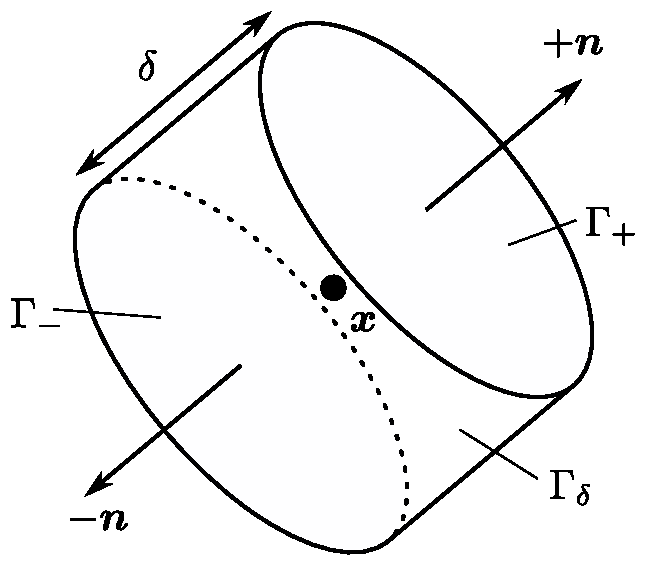
\includegraphics[width=0.6\linewidth,height=\textheight,keepaspectratio]{index_files/mediabag/figs/Omegadelta.pdf}

}

\caption{Illustration of \(\Omega_\delta\) used in the proof of
Proposition~\ref{prp-actionreaction}.}

\end{figure}%

\begin{proposition}[]\protect\hypertarget{prp-actionreaction}{}\label{prp-actionreaction}

Let \({\boldsymbol{t}}:{\mathcal{N}}\times B\to{\mathcal{V}}\) be the
traction function for a body \(B\). Suppose that
\({\boldsymbol{t}}({\boldsymbol{n}},{\boldsymbol{x}})\) is continuous,
and for any sequence of subsets \(\Omega\) whose volumes tend to zero,
we have \begin{equation}\phantomsection\label{eq-arcondition1}{
\frac{1}{{\operatorname{area}}(\partial\Omega)}\int_{\partial\Omega} {\boldsymbol{t}}({\boldsymbol{n}}({\boldsymbol{x}}),{\boldsymbol{x}}){\,\d A_{{\boldsymbol{x}}}}\to\bf0\quad\text{as}\quad{\operatorname{vol}}(\Omega)\to0.
}\end{equation} Then it follows that
\[{\boldsymbol{t}}(-{\boldsymbol{n}},{\boldsymbol{x}}) = -{\boldsymbol{t}}({\boldsymbol{n}},{\boldsymbol{x}})\quad\text{for any }{\boldsymbol{n}}\in{\mathcal{N}},{\boldsymbol{x}}\in B.\]

\end{proposition}

\begin{proof}
Let \({\boldsymbol{x}}\in B\) and \({\boldsymbol{n}}\in{\mathcal{N}}\)
be arbitrary, and let \(D\) be a disc of small radius \(r\), centred at
\({\boldsymbol{x}}\) with normal \({\boldsymbol{n}}\). For \(\delta>0\),
let \(\Omega_\delta\) be the cylinder with centre of volume at
\({\boldsymbol{x}}\), height \(\delta\), and axis parallel to
\({\boldsymbol{n}}\). Let \(\Gamma_{\pm}\) be the circular faces of the
cylinder parallel to \(D\), and the remaining surface be
\(\Gamma_\delta\).

We note that \({\operatorname{area}}(\Gamma_\delta) = 2\pi r\delta\),
which vanishes as \(\delta\to0\), and so
\({\operatorname{area}}(\partial\Omega_\delta)\to 2{\operatorname{area}}(D) = 2\pi r^2\)
as \(\delta\to0\). Note also that
\({\operatorname{vol}}(\Omega_\delta) = \delta \pi r^2\), so
\({\operatorname{vol}}(\Omega_\delta)\to0\) as \(\delta\to0\), so this
sequence of volumes fulfils the assumptions of the proposition, and
since \({\operatorname{area}}(\partial\Omega_\delta)>0\) for all
\(\delta>0\), it follows that
\[\lim_{\delta\to0}\int_{\partial\Omega_\delta} {\boldsymbol{t}}(\widehat{{\boldsymbol{n}}}({\boldsymbol{x}}),{\boldsymbol{x}}')\,dA_{{\boldsymbol{x}}'}=0\]
by assumption.

Next, note that the points in \(\Gamma_\pm\) converge to points in \(D\)
as \(\delta\to0\). Let
\(\widehat{{\boldsymbol{n}}}:\partial\Omega_\delta\to{\mathcal{V}}\) be
the outward unit normal field on \(\partial\Omega_\delta\), so
\(\widehat{{\boldsymbol{n}}}=\pm{\boldsymbol{n}}\) is constant on
\(\Gamma_{\pm}\). We can therefore express
\(\partial\Omega_\delta = \Gamma_\delta\cup\Gamma_+\cup\Gamma_-\), and
since \({\operatorname{area}}(\Gamma_\delta)\to0\) as \(\delta\to0\) and
\({\boldsymbol{t}}\) is continuous and so bounded, we have
\[\lim_{\delta\to0}\int_{\Gamma_\delta} {\boldsymbol{t}}(\widehat{{\boldsymbol{n}}}({\boldsymbol{x}}),{\boldsymbol{x}}')\,dA_{{\boldsymbol{x}}'}=\bf0.\]
It follows that
\[\int_D {\boldsymbol{t}}({\boldsymbol{n}},{\boldsymbol{x}}')+{\boldsymbol{t}}(-{\boldsymbol{n}},{\boldsymbol{x}}')\,dA_{{\boldsymbol{x}}'} = \bf0.\]
Now, we apply the result of Proposition~\ref{prp-MVTsurfaces}, which
allows us to conclude that there is a point
\({\boldsymbol{x}}_r\in D_r\) such that
\[{\boldsymbol{t}}({\boldsymbol{n}},{\boldsymbol{x}}_r)+{\boldsymbol{t}}(-{\boldsymbol{n}},{\boldsymbol{x}}_r)=\bf0.\]
Since this result holds for all \(r>0\), we can now let \(r\to0\). In
this limit, \({\boldsymbol{x}}_r\to {\boldsymbol{x}}\), and since
\({\boldsymbol{t}}\) was assumed to be continuous, it follows that
\[{\boldsymbol{t}}({\boldsymbol{n}},{\boldsymbol{x}})+{\boldsymbol{t}}(-{\boldsymbol{n}},{\boldsymbol{x}})=\bf0.\]
This establishes the result.
\end{proof}

We have just shown that the traction exerted by material on the positive
side of a surface on the negative side is equal and opposite to the
traction exerted by the negative side on the positive. This is Newton's
Third Law in action.

We note that the proof given above does not make complete use of the
full strength of the condition Equation~\ref{eq-arcondition1}, since the
sequence of volumes we consider does not have a vanishing surface area,
but we will use the full strength of this condition in the results which
follow.

\section{The Cauchy stress tensor}\label{the-cauchy-stress-tensor}

Using Proposition~\ref{prp-actionreaction} allows us to say more about
the dependence of the function
\({\boldsymbol{t}}({\boldsymbol{n}},{\boldsymbol{x}})\) upon
\({\boldsymbol{n}}\). This result is often called \emph{Cauchy's
Theorem}, and is fundamental to Continuum Mechanics.

\begin{proposition}[Stress
Tensor]\protect\hypertarget{prp-stresstensor}{}\label{prp-stresstensor}

~

\begin{figure}

{\centering 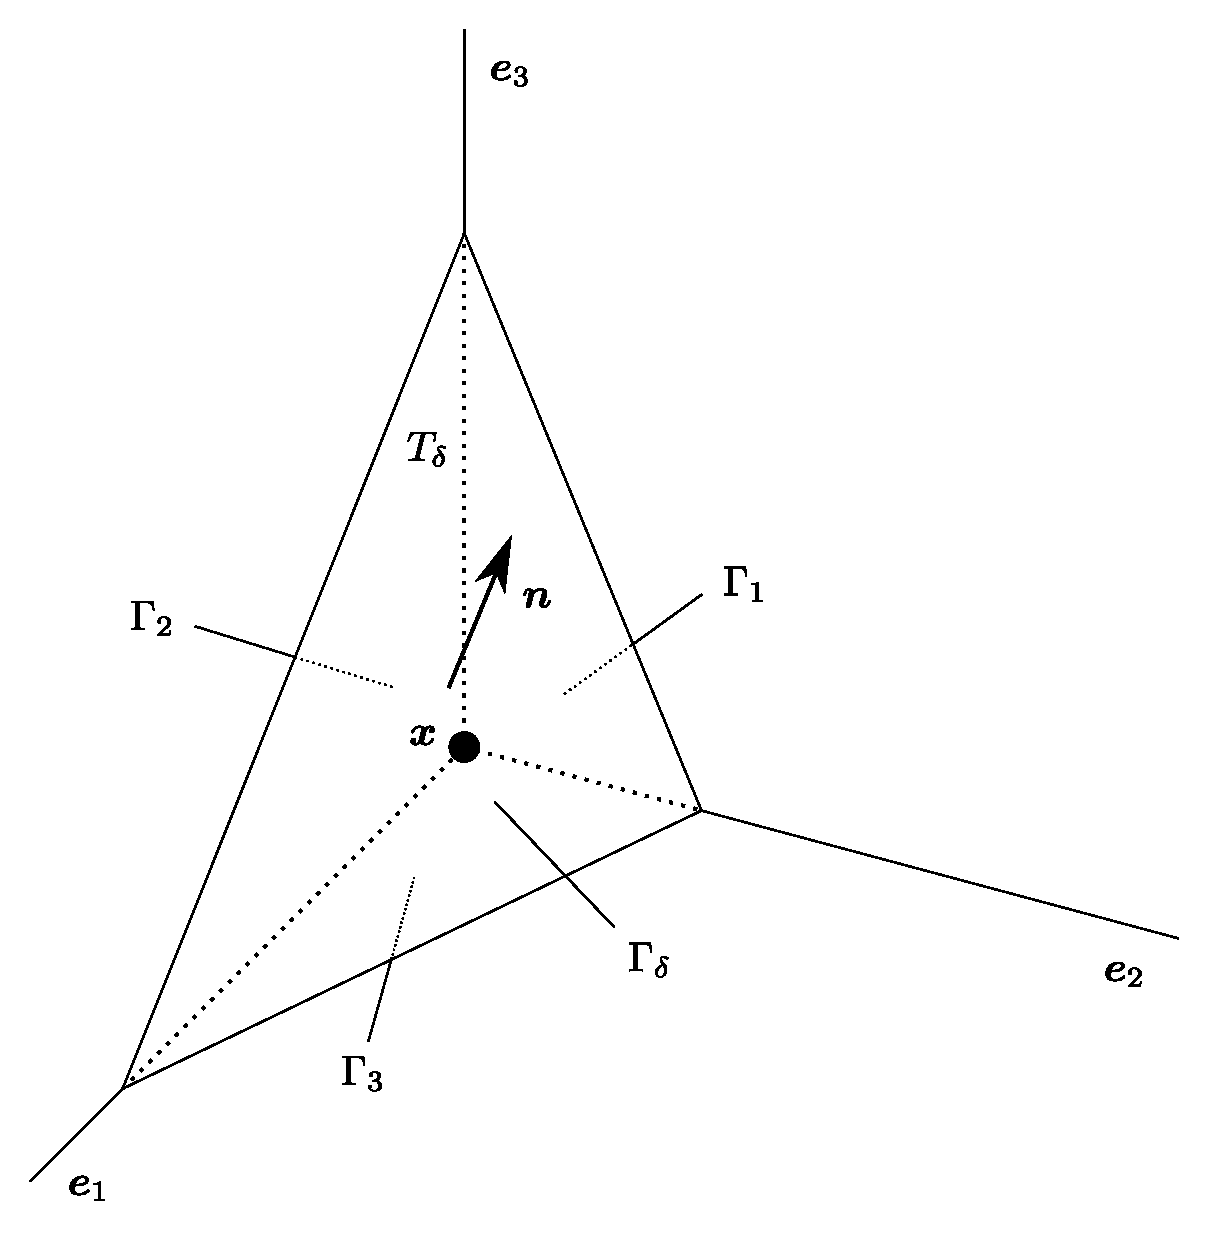
\includegraphics[width=0.9\linewidth,height=\textheight,keepaspectratio]{index_files/mediabag/figs/stresstetrahedron.pdf}

}

\caption{The tetrahedral region used in the proof of
Proposition~\ref{prp-stresstensor}.}

\end{figure}%

Let \({\boldsymbol{t}}:{\mathcal{N}}\times B\to{\mathcal{V}}\) be the
traction function for a body \(B\) which satisfies the conditions of
Proposition~\ref{prp-actionreaction}. Then
\({\boldsymbol{t}}({\boldsymbol{n}},{\boldsymbol{x}})\) is a linear
function of \({\boldsymbol{n}}\), i.e.~for each
\({\boldsymbol{x}}\in B\), there exists a second-order tensor
\({\boldsymbol{S}}({\boldsymbol{x}})\in{\mathcal{V}}^2\) such that
\[{\boldsymbol{t}}({\boldsymbol{n}},{\boldsymbol{x}})= {\boldsymbol{S}}({\boldsymbol{x}}){\boldsymbol{n}}.\]
The field \({\boldsymbol{S}}:B\to{\mathcal{V}}^2\) is called the
\emph{Cauchy stress field} for \(B\).

\end{proposition}

\begin{proof}
We will briefly suspend the summation convention for the first section
of this proof.

Consider an arbitrary Cartesian coordinate frame
\(\{{\boldsymbol{e}}_i\}\), and suppose that
\({\boldsymbol{n}}\cdot{\boldsymbol{e}}_i>0\) for all \(i\). Define the
tetrahedral region
\[T_\delta = \big\{{\boldsymbol{x}}'\in B: 0\leq ({\boldsymbol{x}}'-{\boldsymbol{x}})\cdot{\boldsymbol{e}}_i\text{ and }({\boldsymbol{x}}'-{\boldsymbol{x}})\cdot{\boldsymbol{n}}\leq\delta \big\},\]
which is illustrated in Figure~\hyperref[fig:stresstetradhedron]{1.1}.
\(T_\delta\) has four faces; let the three faces with outward-pointing
unit normal \(-{\boldsymbol{e}}_i\) be denoted \(\Gamma_{\delta,i}\),
and let the final face be denoted \(\Gamma_{\delta,n}\), which has
outward-pointing unit normal \({\boldsymbol{n}}\).

We note that \({\operatorname{vol}}(T_\delta)\to0\) as \(\delta\to0\),
and hence condition~Equation~\ref{eq-arcondition1} implies that
\[\lim_{\delta\to0}\frac{1}{{\operatorname{area}}(\partial T_\delta)}\int_{\partial T_\delta} {\boldsymbol{t}}(\widehat{{\boldsymbol{n}}}({\boldsymbol{x}}'),{\boldsymbol{x}}')\,dA_{{\boldsymbol{x}}'} = \bf0,\]
where \(\widehat{{\boldsymbol{n}}}({\boldsymbol{x}}')\) denotes the
outward-pointing unit normal field on \(\partial T_\delta\). Using the
explicit form for this field on each of the faces, we have
\begin{equation}\phantomsection\label{eq-tetlimit}{
    \lim_{\delta\to0}\frac{1}{{\operatorname{area}}(\partial T_\delta)}\bigg(\int_{\Gamma_{\delta,n}} {\boldsymbol{t}}({\boldsymbol{n}},{\boldsymbol{x}}')\,dA_{{\boldsymbol{x}}'}+\sum_{i=1}^3\int_{\Gamma_{\delta,i}} {\boldsymbol{t}}(-{\boldsymbol{e}}_i,{\boldsymbol{x}}')\,dA_{{\boldsymbol{x}}'}\bigg) = \bf0.}\end{equation}
It can be computed that the area of each face is
\[{\operatorname{area}}(\Gamma_{\delta,i}) = \frac{\delta^2}{2}\frac{n_i}{n_1n_2n_3}\quad\text{and}\quad{\operatorname{area}}(\Gamma_{\delta,n}) = \frac{\delta^2}{2}\frac{1}{n_1n_2n_3},\]
so that \begin{equation}\phantomsection\label{eq-tetarearelation1}{
    {\operatorname{area}}(\Gamma_\delta) = n_1 {\operatorname{area}}(\Gamma_1)=n_2{\operatorname{area}}(\Gamma_2) = n_3{\operatorname{area}}(\Gamma_3),
}\end{equation} and thus
\begin{equation}\phantomsection\label{eq-tetarearelation2}{
    {\operatorname{area}}(\partial T_\delta) = (1+n_1+n_2+n_3){\operatorname{area}}(\Gamma_{\delta,n}).}\end{equation}
We now consider the integral over each face, and apply the Mean Value
Theorem, which entails that there exist points
\({\boldsymbol{x}}'_{\delta,i}\in\Gamma_{\delta,i}\) and a point
\({\boldsymbol{x}}'_{\delta,n}\in\Gamma_{\delta,n}\) such that \$\$

\begin{gathered}
    {\boldsymbol{t}}(-{\boldsymbol{e}}_i,{\boldsymbol{x}}'_{\delta,i}) = \frac{1}{{\operatorname{area}}(\Gamma_{\delta,i})}\int_{\Gamma_{\delta,i}}{\boldsymbol{t}}(-{\boldsymbol{e}}_i,{\boldsymbol{x}}')\,dA_{{\boldsymbol{x}}'}\\
    \text{and}\quad
    {\boldsymbol{t}}({\boldsymbol{n}},{\boldsymbol{x}}'_{\delta,n}) = \frac{1}{{\operatorname{area}}(\Gamma_{\delta,n})}\int_{\Gamma_{\delta,i}}{\boldsymbol{t}}({\boldsymbol{n}},{\boldsymbol{x}}')\,dA_{{\boldsymbol{x}}'}.
  
\end{gathered}

\$\$ We note that as \(\delta\to0\), we have that
\({\boldsymbol{x}}'_{\delta,n}\to{\boldsymbol{x}}\) and
\({\boldsymbol{x}}'_{\delta,i}\to{\boldsymbol{x}}\), since the faces
shrink to the point \({\boldsymbol{x}}\).

Using these facts and Equation~\ref{eq-tetarearelation1}, we have
\[\begin{gathered}
    \int_{\Gamma_{\delta,n}} {\boldsymbol{t}}({\boldsymbol{n}},{\boldsymbol{x}}')\,dA_{{\boldsymbol{x}}'}+\sum_{i=1}^3\int_{\Gamma_{\delta,i}} {\boldsymbol{t}}(-{\boldsymbol{e}}_i,{\boldsymbol{x}}')\,dA_{{\boldsymbol{x}}'}\\
    = {\operatorname{area}}(\Gamma_{\delta,n})\bigg({\boldsymbol{t}}({\boldsymbol{n}},{\boldsymbol{x}}'_{\delta,n})+\sum_{i=1}^3n_i{\boldsymbol{t}}(-{\boldsymbol{e}}_i,{\boldsymbol{x}}_{\delta,i})\bigg).  
\end{gathered}\] Dividing by
\({\operatorname{area}}(\partial T_\delta)\), and applying
Equation~\ref{eq-tetarearelation2} with the limit, we deduce that
\[{\boldsymbol{t}}({\boldsymbol{n}},{\boldsymbol{x}})+\sum_{i=1}^3n_i{\boldsymbol{t}}(-{\boldsymbol{e}}_i,{\boldsymbol{x}}) = \bf0.\]
Applying Proposition~\ref{prp-actionreaction}, and reinstating the
summation convention, this can be rewritten as
\[{\boldsymbol{t}}({\boldsymbol{n}},{\boldsymbol{x}}) = n_i{\boldsymbol{t}}({\boldsymbol{e}}_i,{\boldsymbol{x}}) = \Big({\boldsymbol{t}}({\boldsymbol{e}}_i,{\boldsymbol{x}})\otimes{\boldsymbol{e}}_i\Big){\boldsymbol{n}}={\boldsymbol{S}}({\boldsymbol{x}}){\boldsymbol{n}}\]
where we define
\begin{equation}\phantomsection\label{eq-stresstensordefinition}{
    {\boldsymbol{S}}({\boldsymbol{x}}) = {\boldsymbol{t}}({\boldsymbol{e}}_i,{\boldsymbol{x}})\otimes{\boldsymbol{e}}_i.
}\end{equation} This demonstrates the result for all
\({\boldsymbol{n}}\) such that
\({\boldsymbol{n}}\cdot{\boldsymbol{e}}_i>0\).

To show the result for all remaining vectors, we can first repeat the
argument above for any \({\boldsymbol{n}}\) such that
\({\boldsymbol{n}}\cdot{\boldsymbol{e}}_i\neq0\) by changing frame
\(\{{\boldsymbol{e}}_i\}\) to \(\{{\boldsymbol{e}}_i'\}\) by a sequence
of \(90^\circ\) rotations of the axes. To include vectors for which
\({\boldsymbol{n}}\cdot{\boldsymbol{e}}_i=0\) for at least one \(i\), we
can use the fact that \({\boldsymbol{t}}\) is a assumed to be
continuous.
\end{proof}

From now on, we will abbreviate notation for
\({\boldsymbol{t}}({\boldsymbol{n}}({\boldsymbol{x}}),{\boldsymbol{x}})\),
writing \({\boldsymbol{t}}({\boldsymbol{x}})\), where the dependence on
the normal field \({\boldsymbol{n}}\) is kept implicit, and so we have
\({\boldsymbol{t}}({\boldsymbol{x}}) = {\boldsymbol{S}}({\boldsymbol{x}}){\boldsymbol{n}}\),
or in some cases suppress all arguments to write
\({\boldsymbol{t}}={\boldsymbol{S}}{\boldsymbol{n}}\).

The nine components of the stress tensor
\({\boldsymbol{S}}({\boldsymbol{x}})\) can be understood as the
components of the three traction vectors
\({\boldsymbol{t}}({\boldsymbol{e}}_i,{\boldsymbol{x}})\) acting across
the coordinate planes at the point \({\boldsymbol{x}}\). In particular,
taking components in Equation~\ref{eq-stresstensordefinition}, we have
\[{\boldsymbol{S}}({\boldsymbol{x}}) = S_{ij}({\boldsymbol{x}}){\boldsymbol{e}}_i\otimes{\boldsymbol{e}}_j\quad\text{with}\quad S_{ij}({\boldsymbol{x}}) = t_i({\boldsymbol{e}}_j,{\boldsymbol{x}}),\]
and so
\[{\boldsymbol{t}}({\boldsymbol{e}}_j,{\boldsymbol{x}}) = t_i({\boldsymbol{e}}_j,{\boldsymbol{x}}){\boldsymbol{e}}_i = S_{ij}({\boldsymbol{x}}){\boldsymbol{e}}_i.\]

\section{Equilibrium}\label{equilibrium}

In this section, we define what is meant by a state of mechanical
equilibrium, and use the definition to derive differential equations
satisfied.

\subsection{Preliminaries}\label{preliminaries-3}

Consider a body \(B_0\) in Euclidean space \({\mathbb{E}}^3\), which is
at a state of rest. Suppose the body is then subjected to an external
traction and body force fields which cause the body to change shape and
come to rest in a possibly different configuration \(B\). The mass
density field in the latter configuration is denoted
\(\rho:B\to{\mathbb{R}}\), the external traction field per unit area is
\({\boldsymbol{h}}:\partial B\to{\mathcal{V}}\), and the body force
field per unit mass is \({\boldsymbol{b}}:B\to{\mathcal{V}}\). All of
these fields are assumed not to depend on time.

\subsection{Necessary conditions}\label{necessary-conditions}

Let \(\Omega\subseteq B\) be any open subset of \(B\) and let
\({\boldsymbol{t}}:\partial\Omega\to{\mathcal{V}}\) be the traction
field acting on its outer surface, with orientation determined by the
outward-point normal field. The resultant force on \(\Omega\) due to
body and surface forces is
\begin{equation}\phantomsection\label{eq-resultantforce}{
  {\boldsymbol{r}}(\Omega) = {\boldsymbol{r}}_b(\Omega)+{\boldsymbol{r}}_s(\partial\Omega) = \int_\Omega \rho({\boldsymbol{x}}){\boldsymbol{b}}({\boldsymbol{x}}){\,\d V_{{\boldsymbol{x}}}}+\int_{\partial\Omega}{\boldsymbol{t}}({\boldsymbol{x}}){\,\d A_{{\boldsymbol{x}}}},}\end{equation}
and the resultant torque on \(\Omega\) about the point
\({\boldsymbol{z}}\in{\mathbb{E}}^3\) is
\begin{equation}\phantomsection\label{eq-resultanttorque}{
  \begin{aligned}
    {\boldsymbol{\tau}}(\Omega;{\boldsymbol{z}})
    &= {\boldsymbol{\tau}}_b(\Omega;{\boldsymbol{z}})+{\boldsymbol{\tau}}_s(\partial\Omega;{\boldsymbol{z}})\\
    &=\int_\Omega ({\boldsymbol{x}}-{\boldsymbol{z}})\times\rho({\boldsymbol{x}}){\boldsymbol{b}}({\boldsymbol{x}}){\,\d V_{{\boldsymbol{x}}}}+\int_{\partial \Omega}({\boldsymbol{x}}-{\boldsymbol{x}})\times{\boldsymbol{t}}({\boldsymbol{x}}){\,\d A_{{\boldsymbol{x}}}}.
  \end{aligned}
  }\end{equation} At a static equilibrium, we assume that both the
resultant force and torque for any \(\Omega\) vanish, which is encoded
in the following axiom.

\phantomsection\label{ax:staticequilibrium}{} If a body \(B\) is in a
state of \emph{static mechanical equilibrium}, then the resultant force
and resultant torque (taken about any fixed point) which act on any
sub-body must vanish. That is, it holds that
\begin{equation}\phantomsection\label{eq-equilibriumconditionsINT}{
    \begin{gathered}
      {\boldsymbol{r}}(\Omega)=\int_\Omega \rho({\boldsymbol{x}}){\boldsymbol{b}}({\boldsymbol{x}}){\,\d V_{{\boldsymbol{x}}}}+\int_{\partial\Omega}{\boldsymbol{t}}({\boldsymbol{x}}){\,\d A_{{\boldsymbol{x}}}}=\bf0\\
      {\boldsymbol{\tau}}(\Omega;{\boldsymbol{z}}) = \int_\Omega ({\boldsymbol{x}}-{\boldsymbol{z}})\times\rho({\boldsymbol{x}}){\boldsymbol{b}}({\boldsymbol{x}}){\,\d V_{{\boldsymbol{x}}}}+\int_{\partial \Omega}({\boldsymbol{x}}-{\boldsymbol{z}})\times{\boldsymbol{t}}({\boldsymbol{x}}){\,\d A_{{\boldsymbol{x}}}}=\bf0
    \end{gathered}}\end{equation} for any \(\Omega\subseteq B\).

The fact that we have freedom of choice in choosing the point
\({\boldsymbol{z}}\) in the second equation above is a consequence of
the first equation: see Exercises for details.

\subsection{Local equations}\label{local-equations}

We now use
Axiom~\hyperref[ax:staticequilibrium]{{[}ax:staticequilibrium{]}} to
derive differential equations which are the `local' form of the
equilibrium conditions. Since Proposition~\ref{prp-stresstensor} asserts
that \({\boldsymbol{t}}\) is expressed in terms of the Cauchy stress
tensor \({\boldsymbol{S}}\), it is unsurprising that these equations
naturally involve this field.

\begin{proposition}[]\protect\hypertarget{prp-staticequilibriumeqns}{}\label{prp-staticequilibriumeqns}

If the Cauchy stress field \({\boldsymbol{S}}:B\to{\mathcal{V}}^2\) is
continuously differentiable, and the density field
\(\rho:B\to{\mathbb{R}}\) and body force field \({\boldsymbol{b}}\) are
continuous, then the equilibrium conditions
\hyperref[eq:equilibriumconditionsINT]{{[}eq:equilibriumconditionsINT{]}}
are equivalent to \[\label{eq:equilibriumequationsDE}
    \begin{gathered}
      (\nabla\cdot{\boldsymbol{S}})({\boldsymbol{x}})+\rho({\boldsymbol{x}}){\boldsymbol{b}}({\boldsymbol{x}}) = \bf0 \\
      {\boldsymbol{S}}^T({\boldsymbol{x}})={\boldsymbol{S}}({\boldsymbol{x}})
    \end{gathered}\] for any \({\boldsymbol{x}}\in B\). In components,
these equations are: \[\begin{gathered}
      S_{ij,j}({\boldsymbol{x}})+\rho({\boldsymbol{x}})b_i({\boldsymbol{x}}) = 0 \\
      S_{ij}({\boldsymbol{x}})=S_{ji}({\boldsymbol{x}})
    \end{gathered}\]

\end{proposition}

\begin{proof}
To establish the first equation in
\hyperref[eq:equilibriumequationsDE]{{[}eq:equilibriumequationsDE{]}}
assuming that
Axiom~\hyperref[ax:staticequilibrium]{{[}ax:staticequilibrium{]}} holds,
we first use the definition of \({\boldsymbol{S}}\) to write the first
equation in
\hyperref[eq:equilibriumconditionsINT]{{[}eq:equilibriumconditionsINT{]}}
as
\[\int_{\partial \Omega}{\boldsymbol{S}}{\boldsymbol{n}}{\,\d A_{{\boldsymbol{x}}}}+\int_\Omega\rho{\boldsymbol{b}}{\,\d V_{{\boldsymbol{x}}}}=\bf0.\]
Applying the Tensor Divergence Theorem
Proposition~\ref{prp-tensordivthm} to the first integral, we obtain
\[\int_\Omega \big(\nabla\cdot{\boldsymbol{S}}+\rho{\boldsymbol{b}}\big){\,\d V_{{\boldsymbol{x}}}}=\bf0.\]
Since this equation hold for an arbitrary open set
\(\Omega\subseteq B\), the Localisation Theorem
(Proposition~\ref{prp-localisation}) allows us to conclude that the
integrand vanishes, which is exactly the first result.

To establish the second result, we write the second equation in
\hyperref[eq:equilibriumconditionsINT]{{[}eq:equilibriumconditionsINT{]}}
as
\[\int_{\partial\Omega} ({\boldsymbol{x}}-{\boldsymbol{z}})\times ({\boldsymbol{S}}{\boldsymbol{n}}){\,\d A_{{\boldsymbol{x}}}}+\int_\Omega ({\boldsymbol{x}}-{\boldsymbol{z}})\times\rho{\boldsymbol{b}}{\,\d V_{{\boldsymbol{x}}}}=\bf0.\]
Since we have just shown
\(\rho{\boldsymbol{b}}=-\nabla\cdot{\boldsymbol{S}}\), we can
substitute, and rewrite \[
    \int_{\partial\Omega} ({\boldsymbol{x}}-{\boldsymbol{z}})\times ({\boldsymbol{S}}{\boldsymbol{n}}){\,\d A_{{\boldsymbol{x}}}}-\int_\Omega ({\boldsymbol{x}}-{\boldsymbol{z}})\times\big(\nabla\cdot{\boldsymbol{S}}\big){\,\d V_{{\boldsymbol{x}}}}=\bf0.\]
\{\#eq-equilibriumproof1\} Next, note that we may define the tensor
\({\boldsymbol{R}}=R_{il}{\boldsymbol{e}}_i\otimes{\boldsymbol{e}}_l\)
to be \[R_{il} = \epsilon_{ijk}(x_j-z_j)S_{kl},\] which has the property
that
\({\boldsymbol{R}}{\boldsymbol{n}}=({\boldsymbol{x}}-{\boldsymbol{z}})\times({\boldsymbol{S}}{\boldsymbol{n}})\),
and hence \hyperref[eq:equilibriumproof1]{{[}eq:equilibriumproof1{]}}
can be written as
\[\int_{\partial\Omega}{\boldsymbol{R}}{\boldsymbol{n}}{\,\d A_{{\boldsymbol{x}}}}-\int_\Omega ({\boldsymbol{x}}-{\boldsymbol{z}})\times(\nabla\cdot {\boldsymbol{S}}){\,\d V_{{\boldsymbol{x}}}}=\bf0.\]
Applying the Tensor Divergence Theorem to the first of these integrals,
we find that
\[\int_\Omega\nabla\cdot {\boldsymbol{R}}- ({\boldsymbol{x}}-{\boldsymbol{z}})\times(\nabla\cdot {\boldsymbol{S}}){\,\d V_{{\boldsymbol{x}}}}=\bf0.\]
Applying the Localisation Theorem in the same way as we did above, it
follows that
\[\big(\nabla\cdot{\boldsymbol{R}}\big)({\boldsymbol{x}})-({\boldsymbol{x}}-{\boldsymbol{z}})\times(\nabla\cdot{\boldsymbol{S}})({\boldsymbol{x}})=\bf0\]
for all \({\boldsymbol{x}}\in B\), which in components becomes
\[(\epsilon_{ijk}(x_j-z_j)S_{kl})_{,l}-\epsilon_{ijk}(x_j-z_j)S_{kl,l}=0.\]
Using the product rule, we have \$\$

\begin{aligned}
    &(\epsilon_{ijk}(x_j-z_j)S_{kl})_{,l}-\epsilon_{ijk}(x_j-z_j)S_{kl,l}\\
    &\quad\qquad=\epsilon_{ijk}x_{j,l}S_{kl}+\epsilon_{ijk}(x_j-z_j)S_{kl,l}-\epsilon_{ijk}(x_j-z_j)S_{kl,l}\\
    &\quad\qquad=\epsilon_{ijk}\delta_{jl}S_{kl}\\
    &\quad\qquad=\epsilon_{ilk}S_{kl}
  
\end{aligned}

\[ Considering each of these equations for $i=1,2,3$, we
see that
\]S\_\{32\}-S\_\{23\}=0,\quad S\_\{13\}-S\_\{31\}=0\quad\text{and}\quad S\_\{21\}-S\_\{12\}=0.\$\$
In summary, we have shown that \(S_{ij}=S_{ji}\), and hence
\({\boldsymbol{S}}({\boldsymbol{x}})={\boldsymbol{S}}^T({\boldsymbol{x}})\)
for all \({\boldsymbol{x}}\in B\), which is precisely the second
equation in
\hyperref[eq:equilibriumequationsDE]{{[}eq:equilibriumequationsDE{]}}.

To show that
\hyperref[eq:equilibriumconditionsINT]{{[}eq:equilibriumconditionsINT{]}}
hold starting from
\hyperref[eq:equilibriumequationsDE]{{[}eq:equilibriumequationsDE{]}},
we need simply reverse the arguments above.
\end{proof}

\begin{enumerate}
\def\labelenumi{\arabic{enumi}.}
\item
  The Cauchy stress field is always symmetric, even when a body is not
  in equilibrium (see later).
\item
  The local equilibrium equations
  \hyperref[eq:equilibriumequationsDE]{{[}eq:equilibriumequationsDE{]}}
  do not completely determine the stress field for a body in
  equilibrium, since there are 3 PDEs and 3 algebraic equations for 9
  unknown components of \({\boldsymbol{S}}\). This demonstrates that we
  need additional information to determine the Cauchy stress, and we may
  address this by prescribing \emph{constitutive equations}
  characterising the specific material properties of a body.
\item
  The traction field \({\boldsymbol{h}}\) acting on \(\partial B\)
  represents the surface force per unit area exterted on \(B\) by its
  environment. Applying Proposition~\ref{prp-stresstensor}, we have
  \({\boldsymbol{S}}{\boldsymbol{n}}={\boldsymbol{h}}\) for any
  \({\boldsymbol{x}}\in\partial B\), where \({\boldsymbol{n}}\) is the
  outward-point normal vector on \(\partial B\). This equation provides
  a boundary condition for the local equilibrium equations
  \hyperref[eq:equilibriumequationsDE]{{[}eq:equilibriumequationsDE{]}}.
\item
  In deriving the equilibrium equations, we assumed that the mass
  density \(\rho\) and body force field \({\boldsymbol{b}}\) are
  continuous, and that \({\boldsymbol{S}}\) is continuously
  differentiable. In practice, establishing such regularity properties
  is an important part of the subject, and a topic of active research.
  In this module, we will assume that all fields are sufficiently
  regular to allow us to exchange integral laws for differential
  equations and vice versa.
\end{enumerate}

\section{Stress concepts}\label{stress-concepts}

We now study stress in more detail, describing various states of stress
which may exist at a point in a body. We also discuss the decomposition
of the stress into various components which have important physical
meaning.

\subsection{Simple stress states}\label{simple-stress-states}

If the stress tensor \({\boldsymbol{S}}\) at a point
\({\boldsymbol{x}}\in B\) takes the form
\[{\boldsymbol{S}}= -\pi{\boldsymbol{I}},\] where \(\pi\) is a scalar,
we say that a \emph{spherical} state of stress exists at
\({\boldsymbol{x}}\). In this stress state, the traction on any surface
is parallel to the normal vector \({\boldsymbol{n}}\):
\[{\boldsymbol{t}}= {\boldsymbol{S}}{\boldsymbol{n}}= -\pi{\boldsymbol{n}}.\]

The stress at a point \({\boldsymbol{x}}\in B\) is said to be
\emph{uniaxial} is there exists a unit vector \({\boldsymbol{e}}\) and a
scalar \(\sigma\) such that
\[{\boldsymbol{S}}= \sigma {\boldsymbol{e}}\otimes{\boldsymbol{e}}.\] If
\(\sigma>0\), we call this state a \emph{pure tension}, and if
\(\sigma<0\), a \emph{pure compression}. In this case, the traction on a
surface with normal \({\boldsymbol{n}}\) at \({\boldsymbol{x}}\) is
\[{\boldsymbol{t}}= {\boldsymbol{S}}{\boldsymbol{n}}= ({\boldsymbol{e}}\cdot{\boldsymbol{n}})\sigma {\boldsymbol{e}}.\]
The traction is always parallel to \({\boldsymbol{e}}\), and vanishes if
\({\boldsymbol{n}}\) is orthogonal to \({\boldsymbol{e}}\).

If there are a pair of orthogonal unit vectors \({\boldsymbol{a}}\) and
\({\boldsymbol{b}}\) and a scalar \(\tau\) such that the stress at a
point \({\boldsymbol{x}}\in B\) takes the form
\[{\boldsymbol{S}}=\tau\big({\boldsymbol{a}}\otimes{\boldsymbol{b}}+{\boldsymbol{b}}\otimes{\boldsymbol{a}}),\]
then we say that a state of \emph{pure shear} exists at
\({\boldsymbol{x}}\). For this stress state, the traction on a surface
with normal \({\boldsymbol{n}}\) is
\[{\boldsymbol{t}}= {\boldsymbol{S}}{\boldsymbol{n}}= \tau ({\boldsymbol{b}}\cdot{\boldsymbol{n}}){\boldsymbol{a}}+\tau ({\boldsymbol{a}}\cdot{\boldsymbol{n}}){\boldsymbol{b}}.\]
When \({\boldsymbol{n}}={\boldsymbol{a}}\),
\({\boldsymbol{t}}=\tau{\boldsymbol{b}}\) and when
\({\boldsymbol{n}}={\boldsymbol{b}}\),
\({\boldsymbol{t}}=\tau{\boldsymbol{a}}\).

If at a point \({\boldsymbol{x}}\in B\) there are a pair of orthogonal
unit vectors \({\boldsymbol{a}}\) and \({\boldsymbol{b}}\) such that the
matrix representation of \({\boldsymbol{S}}\) with respect to the basis
\({\boldsymbol{e}}_1={\boldsymbol{a}}\),
\({\boldsymbol{e}}_2={\boldsymbol{b}}\) and
\({\boldsymbol{e}}_3={\boldsymbol{a}}\times{\boldsymbol{b}}\) is
\[= \left(
    \begin{array}{ccc}
      S_{11} & S_{12} & 0 \\
      S_{21} & S_{22} & 0 \\
      0     & 0     & 0
    \end{array}\right),\] we say that a state of \emph{plane stress}
exists at \({\boldsymbol{x}}\).

\subsection{Principal, normal and shear
stresses}\label{principal-normal-and-shear-stresses}

The eigenvalues of the Cauchy stress \({\boldsymbol{S}}\) evaluated at a
point \({\boldsymbol{x}}\in B\) are called the \emph{principal stresses}
at \({\boldsymbol{x}}\). The corresponding eigenvectors are called the
\emph{principal stress directions} at \({\boldsymbol{x}}\). We note that
since the stress tensor is symmetric, there exist three real principal
stresses, and three orthogonal principal stress directions for each
point.

Consider a surface with normal in direction \({\boldsymbol{n}}\) at
\({\boldsymbol{x}}\). Then the corresponding traction vector can be
decomposed into two parts: \[\begin{aligned}
    \text{a \emph{normal traction}:}&\qquad&{\boldsymbol{t}}_n &= ({\boldsymbol{t}}\cdot{\boldsymbol{n}}){\boldsymbol{n}},\\
    \text{and a \emph{shear traction}:}&\qquad&{\boldsymbol{t}}_s&= {\boldsymbol{t}}-({\boldsymbol{t}}\cdot{\boldsymbol{n}}){\boldsymbol{n}},
  \end{aligned}\] In particular, we have
\({\boldsymbol{t}}={\boldsymbol{t}}_n+{\boldsymbol{t}}_s\), and we call
\(\sigma_n=|{\boldsymbol{t}}_n|\) the \emph{normal stress} and
\(\sigma_s=|{\boldsymbol{t}}_s|\) the \emph{shear stress} on the surface
with normal \({\boldsymbol{n}}\) at \({\boldsymbol{x}}\).

\subsection{Maximum normal and shear
stresses}\label{maximum-normal-and-shear-stresses}

Given a point \({\boldsymbol{x}}\) in a body of interest, it is often of
interest to understand what surfaces passing through
\({\boldsymbol{x}}\) experience the largest normal and shear stresses.
In practice, this may be relevant due to knowledge about the level at
which a particular material will undergo failure due to stresses of
these types. For example, both high levels of tension (a normal stress
state) and high levels of shear stress can induce cracking, and the
threshold for these two different modes of failure is often different.

\begin{proposition}[]\protect\hypertarget{prp-maxstresses}{}\label{prp-maxstresses}

Suppose that the principal stresses \(\sigma_i\) at a point
\({\boldsymbol{x}}\in B\) are distinct and ordered, with
\[\sigma_1>\sigma_2>\sigma_3.\] Then

\begin{itemize}
\item
  The maximum normal stress \(\sigma_n\) is \(\max_i|\sigma_i|\).
\item
  The maximum shear stress \(\sigma_s\) is
  \(\frac12|\sigma_1-\sigma_3|\), and this is achieved for for the two
  pairs of normals
  \[{\boldsymbol{n}}= \pm\frac{1}{\sqrt 2}({\boldsymbol{e}}_1+{\boldsymbol{e}}_3)\quad\text{and}\quad{\boldsymbol{n}}= \pm\frac{1}{\sqrt 2}({\boldsymbol{e}}_1-{\boldsymbol{e}}_3).\]
\end{itemize}

\end{proposition}

\subsection{Spherical and deviatoric stress
tensors}\label{spherical-and-deviatoric-stress-tensors}

At any point \({\boldsymbol{x}}\), the Cauchy stress tensor can be
decomposed into two parts, a \emph{spherical stress tensor}
\[{\boldsymbol{S}}_S = -p{\boldsymbol{I}},\] and a \emph{deviatoric
stress tensor}
\[{\boldsymbol{S}}_D = {\boldsymbol{S}}+p{\boldsymbol{I}}= {\boldsymbol{S}}-{\boldsymbol{S}}_S,\]
where \(p=-\frac13{\operatorname{tr}}{\boldsymbol{S}}\) is called the
pressure. Note that
\({\boldsymbol{S}}={\boldsymbol{S}}_S+{\boldsymbol{S}}_D\).

\bookmarksetup{startatroot}

\chapter{Kinematics}\label{sec-kinematics}

\newcommand{\bfa}{{\boldsymbol{a}}}
\newcommand{\bfb}{{\boldsymbol{b}}}
\newcommand{\bfc}{{\boldsymbol{c}}}
\newcommand{\bfd}{{\boldsymbol{d}}}
\newcommand{\bfe}{{\boldsymbol{e}}}
\newcommand{\bff}{{\boldsymbol{f}}}
\newcommand{\bfg}{{\boldsymbol{g}}}
\newcommand{\bfh}{{\boldsymbol{h}}}
\newcommand{\bfi}{{\boldsymbol{i}}}
\newcommand{\bfj}{{\boldsymbol{j}}}
\newcommand{\bfk}{{\boldsymbol{k}}}
\newcommand{\bfl}{{\boldsymbol{l}}}
\newcommand{\bfm}{{\boldsymbol{m}}}
\newcommand{\bfn}{{\boldsymbol{n}}}
\newcommand{\bfo}{{\boldsymbol{o}}}
\newcommand{\bfp}{{\boldsymbol{p}}}
\newcommand{\bfq}{{\boldsymbol{q}}}
\newcommand{\bfr}{{\boldsymbol{r}}}
\newcommand{\bfs}{{\boldsymbol{s}}}
\newcommand{\bft}{{\boldsymbol{t}}}
\newcommand{\bfu}{{\boldsymbol{u}}}
\newcommand{\bfv}{{\boldsymbol{v}}}
\newcommand{\bfw}{{\boldsymbol{w}}}
\newcommand{\bfx}{{\boldsymbol{x}}}
\newcommand{\bfy}{{\boldsymbol{y}}}
\newcommand{\bfz}{{\boldsymbol{z}}}

\newcommand{\bfA}{{\boldsymbol{A}}}
\newcommand{\bfB}{{\boldsymbol{B}}}
\newcommand{\bfC}{{\boldsymbol{C}}}
\newcommand{\bfD}{{\boldsymbol{D}}}
\newcommand{\bfE}{{\boldsymbol{E}}}
\newcommand{\bfF}{{\boldsymbol{F}}}
\newcommand{\bfG}{{\boldsymbol{G}}}
\newcommand{\bfH}{{\boldsymbol{H}}}
\newcommand{\bfI}{{\boldsymbol{I}}}
\newcommand{\bfJ}{{\boldsymbol{J}}}
\newcommand{\bfK}{{\boldsymbol{K}}}
\newcommand{\bfL}{{\boldsymbol{L}}}
\newcommand{\bfM}{{\boldsymbol{M}}}
\newcommand{\bfN}{{\boldsymbol{N}}}
\newcommand{\bfO}{{\boldsymbol{O}}}
\newcommand{\bfP}{{\boldsymbol{P}}}
\newcommand{\bfQ}{{\boldsymbol{Q}}}
\newcommand{\bfR}{{\boldsymbol{R}}}
\newcommand{\bfS}{{\boldsymbol{S}}}
\newcommand{\bfT}{{\boldsymbol{T}}}
\newcommand{\bfU}{{\boldsymbol{U}}}
\newcommand{\bfV}{{\boldsymbol{V}}}
\newcommand{\bfW}{{\boldsymbol{W}}}
\newcommand{\bfX}{{\boldsymbol{X}}}
\newcommand{\bfY}{{\boldsymbol{Y}}}
\newcommand{\bfZ}{{\boldsymbol{Z}}}

\newcommand{\bftau}{{\boldsymbol{\tau}}}
\newcommand{\bfnu}{{\boldsymbol{\nu}}}
\newcommand{\bfpsi}{{\boldsymbol{\psi}}}
\newcommand{\bfphi}{{\boldsymbol{\varphi}}}
\newcommand{\bfSigma}{{\boldsymbol{\Sigma}}}
\newcommand{\calI}{{\mathcal{I}}}
\newcommand{\calN}{{\mathcal{N}}}
\newcommand{\calV}{{\mathcal{V}}}
\newcommand{\bbE}{{\mathbb{E}}}
\newcommand{\bbR}{{\mathbb{R}}}
\newcommand{\bbC}{{\mathbb{C}}}
\newcommand{\bsfC}{{\mathsf{C}}}
\newcommand{\bsfD}{{\mathsf{D}}}
\newcommand{\bsfI}{{\mathsf{I}}}
\newcommand{\bsfO}{{\mathsf{O}}}
\newcommand{\tr}{{\operatorname{tr}}}
\newcommand{\sym}{{\operatorname{sym}}}
\newcommand{\skw}{{\operatorname{skew}}}
\newcommand{\vc}{{\operatorname{vec}}}
\newcommand{\ten}{{\operatorname{ten}}}
\newcommand{\cof}{{\operatorname{cof}}}
\newcommand{\mass}{{\operatorname{mass}}}
\newcommand{\vol}{{\operatorname{vol}}}
\newcommand{\area}{{\operatorname{area}}}
\newcommand{\com}{{\operatorname{com}}}
\newcommand{\cov}{{\operatorname{cov}}}
\newcommand{\e}{{\mathrm{e}}}
\newcommand{\D}{{\mathrm{D}}}
\newcommand{\dd}{{\mathrm{d}}}
\newcommand{\dt}{{\dd t}}
\newcommand{\Dt}{{\D t}}
\newcommand{\bigO}{{O}}
\newcommand{\litO}{{o}}
\newcommand{\dVx}{{\,\d V_{\bfx}}}
\newcommand{\dAx}{{\,\d A_{\bfx}}}
\newcommand{\dVy}{{\,\d V_{\bfy}}}
\newcommand{\dAy}{{\,\d A_{\bfy}}}
\newcommand{\ds}{{\,\d s}}

\section{Preliminaries}\label{preliminaries-4}

Kinematics is the study of describing motion independently of
considering mass, forces and stress. We describe the notion of strain in
a body which changes shape over time. In the remainder of the module, we
will discuss particular relationships between stress and strain which
characterise different types of materials.

\textbf{Aims.} By the end of this chapter, you should be able to:

\begin{itemize}
\item
  Define and geometrically interpret the \emph{deformation gradient},
  \emph{Cauchy-Green strain tensor}, and the \emph{infinitesimal strain
  tensor}.
\item
  Use the concept of a \emph{motion} to describe the change in a body.
\item
  Describe the relationship between \emph{material} and \emph{spatial
  fields}.
\item
  Define the \emph{total time derivative} of material and spatial
  fields.
\item
  Define the \emph{velocity}, \emph{acceleration}, \emph{vorticity},
  \emph{rate of strain} and \emph{spin} fields.
\item
  Explain how volume and surface integrals of fields transform and
  change due to motion thanks to \emph{change of variables formulae} and
  the \emph{Reynolds Transport Theorem}.
\end{itemize}

\section{Configurations and
deformations}\label{configurations-and-deformations}

At any particular time, a material body occupies an open subset
\(B\subseteq{\mathbb{E}}^3\), as discussed in
Chapter~\ref{sec-mass-forces}. The identification of material particles
with point of \(B\) defines what is called a \emph{configuration} of the
body.

A \emph{deformation} is a mapping between two configurations, usually a
fixed region \(B\) called the \emph{reference configuration} and another
varying configuration \(B'\) called the \emph{deformed configuration}.
We will denote points in \(B\) by \({\boldsymbol{x}}\), and points in
\(B'\) by \({\boldsymbol{y}}\). If we view \(B\) and \(B'\) as two
configurations of the same material body, we expect that there is a
one-to-one correspondence between points in the two configurations.

This leads us naturally to the idea of the deformation map. We will
describe the mapping from \(B\) to \(B'\) by a function
\({\boldsymbol{y}}:B\to B'\) which maps each point \({\boldsymbol{x}}\)
to a point \({\boldsymbol{y}}({\boldsymbol{x}})\in B'\). The
displacement of a material particle from its initial location
\({\boldsymbol{x}}\) to final location
\({\boldsymbol{y}}({\boldsymbol{x}})\) is
\[{\boldsymbol{u}}({\boldsymbol{x}}) = {\boldsymbol{y}}({\boldsymbol{x}})-{\boldsymbol{x}}.\]
We call \({\boldsymbol{u}}:B\to{\mathcal{V}}\) the \emph{displacement
field} associated to \({\boldsymbol{y}}\).

We will assume that deformation maps satisfy the following two important
conditions:

\begin{itemize}
\item
  \({\boldsymbol{y}}:B\to B'\) is one-to-one, and
\item
  \(\det\nabla{\boldsymbol{y}}({\boldsymbol{x}})>0\) for all
  \({\boldsymbol{x}}\in B\).
\end{itemize}

Deformations satisfying both of these assumptions will be called
\emph{admissible deformations}. The first of these assumptions means
that two material particles cannot occupy the same location, and the
second ensures that a body cannot be continuously mapped onto its own
mirror image. Note that the first assumption is sufficient to ensure
that \({\boldsymbol{y}}\) is a bijection between \(B\) and \(B'\).

Throughout, we will assume that all deformations are admissible, and
that all are smooth enough to allow us to justify the operations of
differentiation we need. Finding (and guaranteeing) that these
assumptions hold in particular cases are the topic of active research.

\section{Measures of strain}\label{measures-of-strain}

Consider the open ball \(\Omega\) of radius \(\delta\) centred at
\({\boldsymbol{x}}_0\) within the body we consider. Under the
deformation \({\boldsymbol{y}}\), \({\boldsymbol{x}}_0\) is mapped to
\({\boldsymbol{y}}_0={\boldsymbol{y}}({\boldsymbol{x}}_0)\), and
\(\Omega_\delta\) is mapped to a region
\(\Omega'={\boldsymbol{y}}(\Omega)\). Any difference in shaped between
\(\Omega'\) and \(\Omega\) as \(\delta\to0\) is called \emph{strain} at
\({\boldsymbol{x}}_0\). Strain refers to the local stretching of a body
induced by the deformation \({\boldsymbol{y}}\). The concept of strain
plays a central roles in modelling solid materials.

\subsection{The deformation gradient}\label{the-deformation-gradient}

One way to quantify strain is through the \emph{deformation gradient}, a
second-order tensor field \({\boldsymbol{F}}:B\to{\mathcal{V}}^2\)
defined to be
\[{\boldsymbol{F}}({\boldsymbol{x}}) = \nabla {\boldsymbol{y}}({\boldsymbol{x}}).\]
The field \({\boldsymbol{F}}\) naturally provides information on the
local behaviour of \({\boldsymbol{y}}\), since Taylor expanding, we see
\[{\boldsymbol{y}}({\boldsymbol{x}}) = {\boldsymbol{y}}({\boldsymbol{x}}_0) +{\boldsymbol{F}}({\boldsymbol{x}}_0)({\boldsymbol{x}}-{\boldsymbol{x}}_0)+{O}\big(|{\boldsymbol{x}}-{\boldsymbol{x}}_0|^2\big),\]
or equivalently
\[{\boldsymbol{y}}({\boldsymbol{x}}) = {\boldsymbol{c}}+{\boldsymbol{F}}({\boldsymbol{x}}_0){\boldsymbol{x}}+{O}\big(|{\boldsymbol{x}}-{\boldsymbol{x}}_0|^2\big)\quad\text{where}\quad {\boldsymbol{c}}= {\boldsymbol{y}}({\boldsymbol{x}}_0)-{\boldsymbol{F}}({\boldsymbol{x}}_0){\boldsymbol{x}}_0.\]

To understand better how \({\boldsymbol{F}}\) measures strain, suppose
for simplicity that \({\boldsymbol{y}}\) is \emph{homogeneous}, which
means the deformation gradient field is constant,
i.e.~\[{\boldsymbol{y}}({\boldsymbol{x}}) = {\boldsymbol{c}}+ {\boldsymbol{F}}{\boldsymbol{x}},\]
so the deformation is an \emph{affine map}. We note that by virtue of
this affine nature, any line segment in the reference configuration
\(B\) is mapped onto a corresponding line segment in the deformed
configuration \(B'\).

We also remark that the admissibility conditions we require of
deformations imply that
\(\det\nabla{\boldsymbol{y}}({\boldsymbol{x}})>0\), which ensures that
\(\det{\boldsymbol{F}}>0\), so \({\boldsymbol{F}}\) is invertible.

\subsubsection{Translations and fixed
points}\label{translations-and-fixed-points}

A homogeneous deformation \({\boldsymbol{y}}\) is called a translation
if \({\boldsymbol{F}}={\boldsymbol{I}}\),
i.e.~\[{\boldsymbol{y}}({\boldsymbol{x}}) = {\boldsymbol{x}}+{\boldsymbol{c}}\quad\text{for some fixed }{\boldsymbol{c}}\in{\mathcal{V}}.\]
Under such a deformation, all points in \(B'\) are simply moved through
a displacement \({\boldsymbol{c}}\), so there is no change in shape or
orientation of the body.

A homogeneous deformation has a fixed point at \({\boldsymbol{x}}'\) if
\begin{equation}\phantomsection\label{eq-defFixedPoint}{
  {\boldsymbol{y}}({\boldsymbol{x}}) = {\boldsymbol{x}}'+ {\boldsymbol{F}}({\boldsymbol{x}}-{\boldsymbol{x}}').
}\end{equation} The point \({\boldsymbol{x}}'\) is fixed in the sense
that \({\boldsymbol{y}}({\boldsymbol{x}}') = {\boldsymbol{x}}'\). Any
other point in the body is displaced by an amount determined by
\({\boldsymbol{F}}\) and the position relative to the fixed point
\({\boldsymbol{x}}'\). For such a deformation, the body can change both
shape and orientation. We now define a couple of classes of homogeneous
deformation with fixed points.

A homogeneous deformation \({\boldsymbol{y}}\) is called a
\emph{rotation about \({\boldsymbol{x}}'\)} if it takes the form
\[{\boldsymbol{y}}({\boldsymbol{x}})={\boldsymbol{x}}'+{\boldsymbol{Q}}({\boldsymbol{x}}-{\boldsymbol{x}}')\]
for some rotation tensor \({\boldsymbol{Q}}\in{\mathcal{V}}^2\). Such
deformations change the orientation of the body, but not its shape.

A homogeneous deformation \({\boldsymbol{y}}\) is called a \emph{stretch
about \({\boldsymbol{x}}'\)} if it takes the form
\[{\boldsymbol{y}}({\boldsymbol{x}})={\boldsymbol{x}}'+{\boldsymbol{S}}({\boldsymbol{x}}-{\boldsymbol{x}}')\]
for some symmetric positive definite tensor
\({\boldsymbol{S}}\in{\mathcal{V}}^2\). Under such a deformation, the
orientation of the body is not changed, but it is extended by different
amounts in different directions with the point \({\boldsymbol{x}}'\)
remaining fixed.

The following result shows that an arbitrary homogeneous deformation can
be expressed as a composition of a translation and deformation with a
given fixed point.

Let \({\boldsymbol{y}}\) be a homogeneous deformation. Then, given any
point \({\boldsymbol{x}}'\in{\mathbb{E}}^3\), we can decompose
\({\boldsymbol{y}}\) as
\[{\boldsymbol{y}}= {\boldsymbol{t}}_1\circ {\boldsymbol{g}}={\boldsymbol{g}}\circ{\boldsymbol{t}}_2,\]
where \({\boldsymbol{t}}_1\) and \({\boldsymbol{t}}_2\) are
translations, and \({\boldsymbol{g}}\) is a homogeneous deformation with
a fixed point at \({\boldsymbol{x}}'\). In particular:
\[{\boldsymbol{g}}({\boldsymbol{x}}) = {\boldsymbol{x}}'+{\boldsymbol{F}}({\boldsymbol{x}}-{\boldsymbol{x}}').\]

\begin{proof}
See Exercise Sheet 3.
\end{proof}

We now show that an arbitrary homogeneous deformation with a fixed point
can always be decomposed as a rotation and a stretch about the same
fixed point, using the polar decomposition theorem.

\begin{proposition}[]\protect\hypertarget{prp-stretchdecomposition}{}\label{prp-stretchdecomposition}

If \({\boldsymbol{y}}\) is a homogeneous deformation with a fixed point
\({\boldsymbol{x}}'\) and deformation gradient \({\boldsymbol{F}}\), let
\({\boldsymbol{F}}= {\boldsymbol{R}}{\boldsymbol{U}}={\boldsymbol{V}}{\boldsymbol{R}}\)
be the right and left polar decompositions of \({\boldsymbol{F}}\). Then
\({\boldsymbol{y}}\) can be decomposed as
\[{\boldsymbol{y}}= {\boldsymbol{r}}\circ {\boldsymbol{s}}_1={\boldsymbol{s}}_2\circ{\boldsymbol{r}},\]
where \({\boldsymbol{r}}\) is a rotation about \({\boldsymbol{x}}'\),
and \({\boldsymbol{s}}_1\) and \({\boldsymbol{s}}_2\) are stretches
about \({\boldsymbol{x}}'\). In particular: \[\begin{gathered}
    {\boldsymbol{r}}({\boldsymbol{x}}) = {\boldsymbol{x}}'+{\boldsymbol{R}}({\boldsymbol{x}}-{\boldsymbol{x}}'),\quad{\boldsymbol{s}}_1({\boldsymbol{x}}) = {\boldsymbol{x}}'+{\boldsymbol{U}}({\boldsymbol{x}}-{\boldsymbol{x}}')\\
    \text{and}\quad\quad{\boldsymbol{s}}_2({\boldsymbol{x}}) = {\boldsymbol{x}}'+{\boldsymbol{V}}({\boldsymbol{x}}-{\boldsymbol{x}}').
  \end{gathered}\]

\end{proposition}

\begin{proof}
See Exercise Sheet 3.
\end{proof}

We can go further in decomposing stretches, by making the following
definition. A homogeneous deformation \({\boldsymbol{y}}\) is called an
\emph{extension} about \({\boldsymbol{x}}'\) in the direction of a unit
vector \({\boldsymbol{e}}\) if
\[{\boldsymbol{y}}({\boldsymbol{x}}) = {\boldsymbol{x}}'+{\boldsymbol{F}}({\boldsymbol{x}}-{\boldsymbol{x}}')\quad\text{with}\quad {\boldsymbol{F}}={\boldsymbol{I}}+(\lambda-1){\boldsymbol{e}}\otimes{\boldsymbol{e}},\]
for some \(\lambda>0\). This terminology is based on the observation
that \({\boldsymbol{F}}\) changes the length of any vector parallel to
\({\boldsymbol{e}}\) by a factor of \(\lambda\), that is
\[{\boldsymbol{F}}(\alpha{\boldsymbol{e}}) = \alpha{\boldsymbol{e}}+(\lambda-1)\alpha({\boldsymbol{e}}\cdot{\boldsymbol{e}}){\boldsymbol{e}}= \lambda\alpha{\boldsymbol{e}}\]
This is a particular case of the stretch deformation introduced earlier.
The following result shows that the stretches appearing in
Proposition~\ref{prp-stretchdecomposition} can be expressed as the
composition of three extensions defined by the eigenvalues and
eigenvectors of \({\boldsymbol{U}}\) and \({\boldsymbol{V}}\).

Let \({\boldsymbol{s}}_1\) and \({\boldsymbol{s}}_2\) be the stretches
defined in Proposition~\ref{prp-stretchdecomposition}, and let
\(\{\lambda_i,{\boldsymbol{u}}_i\}\) and
\(\{\lambda_i,{\boldsymbol{v}}_i\}\) be the eigenpairs associated with
the tensors \({\boldsymbol{U}}\) and \({\boldsymbol{V}}\) respectively.
Then
\[{\boldsymbol{s}}_1 = {\boldsymbol{f}}_1\circ{\boldsymbol{f}}_2\circ{\boldsymbol{f}}_3\quad\text{and}\quad{\boldsymbol{s}}_2={\boldsymbol{h}}_1\circ{\boldsymbol{h}}_2\circ{\boldsymbol{h}}_3,\]
where \({\boldsymbol{f}}_i\) is the extension about
\({\boldsymbol{x}}'\) by \(\lambda_i\) in the direction
\({\boldsymbol{u}}_i\), and \({\boldsymbol{h}}_i\) is the extension
about \({\boldsymbol{x}}'\) by \(\lambda_i\) in the direction
\({\boldsymbol{v}}_i\).

\textbf{Exercise:} Prove this result.

Notes:

\begin{enumerate}
\def\labelenumi{\arabic{enumi}.}
\item
  The tensors \({\boldsymbol{U}}\) and \({\boldsymbol{V}}\) which appear
  in the right and left polar decompositions of \({\boldsymbol{F}}\)
  have the same eigenvalues, but (in general) have different
  eigenvectors. It follows that \({\boldsymbol{s}}_1\) and
  \({\boldsymbol{s}}_2\) give rise to extensions by the same amounts,
  but in different directions.
\item
  We call the eigenvalues \(\lambda_i\) the \emph{principal stretches}
  associated with the deformation gradient \({\boldsymbol{F}}\), and the
  eigenvectors \({\boldsymbol{u}}_i\) and \({\boldsymbol{v}}_i\) are
  respectively referred to as the right and left \emph{principal
  directions}. Similarly, we call \({\boldsymbol{U}}\) and
  \({\boldsymbol{V}}\) the right and left \emph{stretch tensors}.
\end{enumerate}

In summary, we have shown that a homogeneous deformation can be
decomposed in various ways, for example as a translation, then a
rotation, then a series of extensions, or as a translation, then a
series of extensions, and then a rotation. These different
decompositions allow us to think about how a body might be affected by
such a sequence of operations, and so devise physically-appropriate
models, especially since a Taylor expansion of the deformation
\({\boldsymbol{y}}\) allows us to treat deformations close to a given
point as approximately homogeneous.

\subsection{The Cauchy--Green strain
tensor}\label{the-cauchygreen-strain-tensor}

Consider a general deformation \({\boldsymbol{y}}:B\to B'\) with
deformation gradient \({\boldsymbol{F}}= \nabla {\boldsymbol{y}}\).
Another measure of strain is the \emph{right Cauchy-Green strain tensor}
field \({\boldsymbol{C}}:B\to{\mathcal{V}}^2\), defined by
\[{\boldsymbol{C}}= {\boldsymbol{F}}^T{\boldsymbol{F}},\] Notice that
\({\boldsymbol{C}}\) is symmetric and positive definite at every point
in \(B\).

While \({\boldsymbol{F}}\) contains information on both rotation and
stretching, \({\boldsymbol{C}}\) including information about stretches
only: since \({\boldsymbol{F}}={\boldsymbol{R}}{\boldsymbol{U}}\),
\[{\boldsymbol{C}}= {\boldsymbol{F}}^T{\boldsymbol{F}}= {\boldsymbol{U}}^2,\]
we see the definition of \({\boldsymbol{C}}\) does not contain
\({\boldsymbol{R}}\).

\begin{itemize}
\item
  Note that \({\boldsymbol{U}}\) is also independent of
  \({\boldsymbol{R}}\), and contains information on stretches only, but
  \({\boldsymbol{C}}\) is easier to compute than the square root
  \({\boldsymbol{U}}=\sqrt{{\boldsymbol{F}}^T{\boldsymbol{F}}}=\sqrt{{\boldsymbol{C}}}\).
\item
  Recall from the Spectral Decomposition Theorem that
  \[{\boldsymbol{U}}= \sum_{i=1}^3 \lambda_i{\boldsymbol{e}}_i\otimes{\boldsymbol{e}}_i,\]
  where \(\lambda_i>0\) and \({\boldsymbol{e}}_i\) are orthonormal
  eigenvectors of \({\boldsymbol{U}}\). As
  \({\boldsymbol{C}}= {\boldsymbol{U}}^2\), we see that
  \[{\boldsymbol{C}}= \sum_{i=1}^3 \lambda_i^2{\boldsymbol{e}}_i\otimes{\boldsymbol{e}}_i,\]
  so the eigenvalues of \({\boldsymbol{C}}\) are the squares of the
  principal stretches.
\item
  Another measure of strain is the \emph{left Cauchy-Green strain
  tensor}, \({\boldsymbol{B}}= {\boldsymbol{F}}{\boldsymbol{F}}^T\). We
  will not use this measure here.
\end{itemize}

We now consider the interpretation of \({\boldsymbol{C}}\). Consider a
point \({\boldsymbol{x}}_0\) in the reference configuration, and let
\(\Omega\) be the open ball of radius \(\alpha>0\) centred at
\({\boldsymbol{x}}_0\). Consider the points
\({\boldsymbol{x}}_1 = {\boldsymbol{x}}_0+\alpha{\boldsymbol{e}}\) and
\({\boldsymbol{x}}_2={\boldsymbol{x}}_0+\alpha{\boldsymbol{d}}\), where
\({\boldsymbol{e}}\) and \({\boldsymbol{d}}\) are unit vectors. Let
\({\boldsymbol{y}}_0={\boldsymbol{y}}({\boldsymbol{x}}_0)\),
\({\boldsymbol{y}}_1={\boldsymbol{y}}({\boldsymbol{x}}_1)\) and
\({\boldsymbol{y}}_2={\boldsymbol{y}}({\boldsymbol{x}}_2)\) be the
corresponding points in the deformed configuration. Let
\(\phi\in[0,\pi]\) be the angle between
\({\boldsymbol{v}}={\boldsymbol{y}}_1-{\boldsymbol{y}}_0\) and
\({\boldsymbol{w}}={\boldsymbol{y}}_2-{\boldsymbol{y}}_0\).

\begin{proposition}[]\protect\hypertarget{prp-CGstrainrelations}{}\label{prp-CGstrainrelations}

For any point \({\boldsymbol{x}}_0\in B\) and unit vectors
\({\boldsymbol{e}}\) and \({\boldsymbol{d}}\), define
\[\lambda({\boldsymbol{e}}) = \sqrt{{\boldsymbol{e}}\cdot{\boldsymbol{C}}{\boldsymbol{e}}}>0 \quad\text{and}\quad
    \theta({\boldsymbol{e}},{\boldsymbol{d}}) = \arccos\bigg(\frac{{\boldsymbol{e}}\cdot{\boldsymbol{C}}{\boldsymbol{d}}}{\sqrt{{\boldsymbol{e}}\cdot{\boldsymbol{C}}{\boldsymbol{e}}}\sqrt{{\boldsymbol{d}}\cdot{\boldsymbol{C}}{\boldsymbol{d}}}}\bigg)\in[0,\pi].\]
Then, as \(\alpha\to0\), we have that
\[\frac{|{\boldsymbol{y}}'-{\boldsymbol{y}}_0|}{|{\boldsymbol{x}}'-{\boldsymbol{x}}_0|}\to\lambda({\boldsymbol{e}}),\quad \frac{|{\boldsymbol{y}}''-{\boldsymbol{y}}_0|}{|{\boldsymbol{x}}''-{\boldsymbol{x}}_0|}\to\lambda({\boldsymbol{d}})\]
and \[\phi\to \theta({\boldsymbol{e}},{\boldsymbol{d}}).\]

\end{proposition}

\begin{proof}
Note that
\({\boldsymbol{v}}= {\boldsymbol{y}}({\boldsymbol{x}}_0+\alpha{\boldsymbol{e}})-{\boldsymbol{y}}({\boldsymbol{x}}_0)\),
so Taylor expanding, we have
\[{\boldsymbol{v}}= \alpha {\boldsymbol{F}}({\boldsymbol{x}}_0){\boldsymbol{e}}+{O}(\alpha^2).\]
It follows that
\[|{\boldsymbol{v}}|^2 = \alpha^2{\boldsymbol{F}}({\boldsymbol{x}}_0){\boldsymbol{e}}\cdot{\boldsymbol{F}}({\boldsymbol{x}}_0){\boldsymbol{e}}+{O}(\alpha^3) = \alpha^2 {\boldsymbol{e}}\cdot{\boldsymbol{C}}({\boldsymbol{x}}_0){\boldsymbol{e}}+{O}(\alpha^3).\]
Dividing through by
\(\alpha^2=|{\boldsymbol{x}}'-{\boldsymbol{x}}_0|^2\), and using the
fact that \({\boldsymbol{v}}={\boldsymbol{y}}'-{\boldsymbol{y}}_0\), we
have
\[\frac{|{\boldsymbol{y}}'-{\boldsymbol{y}}_0|^2}{|{\boldsymbol{x}}'-{\boldsymbol{x}}_0|^2} = \frac{|{\boldsymbol{v}}|^2}{\alpha^2} = {\boldsymbol{e}}\cdot{\boldsymbol{C}}({\boldsymbol{x}}_0){\boldsymbol{e}}+{O}(\alpha),\]
which, after taking a square root, proves the first result. The second
result follows by a similar argument.

To establish the final result, we note that
\[\cos\phi = \frac{{\boldsymbol{v}}\cdot{\boldsymbol{w}}}{|{\boldsymbol{v}}||{\boldsymbol{w}}|}.\]
Using the facts that
\({\boldsymbol{v}}=\alpha{\boldsymbol{F}}({\boldsymbol{x}}){\boldsymbol{e}}+{O}(\alpha^2)\)
and
\({\boldsymbol{w}}=\alpha{\boldsymbol{F}}({\boldsymbol{x}}){\boldsymbol{d}}+{O}(\alpha^2)\),
we have
\[\frac{{\boldsymbol{v}}\cdot{\boldsymbol{w}}}{\alpha^2} = {\boldsymbol{e}}\cdot{\boldsymbol{C}}({\boldsymbol{x}}){\boldsymbol{d}}+{O}(\alpha).\]
Then, using
\(|{\boldsymbol{v}}| = \alpha \lambda({\boldsymbol{e}})+{O}(\alpha^2)\)
and
\(|{\boldsymbol{w}}|=\alpha\lambda({\boldsymbol{d}})+{O}(\alpha^2)\), we
conclude.
\end{proof}

\textbf{Remarks:}

\begin{enumerate}
\def\labelenumi{\arabic{enumi}.}
\item
  This result states that \(\lambda({\boldsymbol{e}})\) approximates the
  ratio of lengths between deformed points and reference points, where
  the reference points are separated by a short displacement in the
  direction \({\boldsymbol{e}}\). This is the reason for naming
  \(\lambda({\boldsymbol{e}})\) the \emph{stretch} in the direction
  \({\boldsymbol{e}}\) at the reference point \({\boldsymbol{x}}\).
\item
  At any fixed reference point \({\boldsymbol{x}}\), the extreme values
  of \(\lambda({\boldsymbol{e}})\) occur when \({\boldsymbol{e}}\) is an
  eigenvector of \({\boldsymbol{C}}\) (i.e. a right principal
  direction). As a result the extreme values of
  \(\lambda({\boldsymbol{e}})\) are given by the maximum and minimum
  principal stretches.
\item
  \(\theta({\boldsymbol{e}},{\boldsymbol{d}})\) approximates the angle
  between points in the deformed configuration which lie at short
  distances from \({\boldsymbol{x}}\) along the directions
  \({\boldsymbol{e}}\) and \({\boldsymbol{d}}\). If
  \(\Theta({\boldsymbol{e}},{\boldsymbol{d}}) = \arccos({\boldsymbol{e}}\cdot{\boldsymbol{d}})\)
  is the angle between these directions in the reference configuration,
  we define
  \[\gamma({\boldsymbol{e}},{\boldsymbol{d}}) = \Theta({\boldsymbol{e}},{\boldsymbol{d}})-\theta({\boldsymbol{e}},{\boldsymbol{d}}),\]
  which we call the \emph{shear} between the directions
  \({\boldsymbol{e}}\) and \({\boldsymbol{d}}\) at the point
  \({\boldsymbol{x}}\). The shear measures the change in angle between
  directions due to deformation.
\end{enumerate}

The following result shows that \({\boldsymbol{C}}\) explicitly
characterises the stretch and shear caused by a deformation.

\begin{proposition}[]\protect\hypertarget{prp-stretchshear}{}\label{prp-stretchshear}

Let \(C_{ij}\) be the components of \({\boldsymbol{C}}\) with respect to
an arbitrary coordinate frame \(\{{\boldsymbol{e}}_i\}\). Then, for any
point \({\boldsymbol{x}}\in B\), we have
\[C_{ii} = \lambda({\boldsymbol{e}}_i)^2\quad\text{and}\quad C_{ij} = \lambda({\boldsymbol{e}}_i)\lambda({\boldsymbol{e}}_j)\sin\big(\gamma({\boldsymbol{e}}_i,{\boldsymbol{e}}_j)\big),\]
where no summation is implied. The diagonal components of
\({\boldsymbol{C}}\) are therefore the squares of the stretches along
coordinate directions, and the off-diagonal components capture the shear
between corresponding pairs of coordinate directions.

\end{proposition}

\subsection{Rigid deformations}\label{rigid-deformations}

A homogeneous deformation \({\boldsymbol{y}}:B\to B'\) is a \emph{rigid
deformation} if
\[{\boldsymbol{y}}({\boldsymbol{x}}) = {\boldsymbol{c}}+{\boldsymbol{Q}}{\boldsymbol{x}}\]
where \({\boldsymbol{c}}\in{\mathcal{V}}\) and
\({\boldsymbol{Q}}\in{\mathcal{V}}^2\) is a rotation tensor. For such
deformations we have \({\boldsymbol{F}}={\boldsymbol{Q}}\), and hence
\[{\boldsymbol{C}}= {\boldsymbol{F}}^T{\boldsymbol{F}}= {\boldsymbol{Q}}^T{\boldsymbol{Q}}= {\boldsymbol{I}}.\]
It follows that rigid deformations produce no strain measured by
\({\boldsymbol{C}}\). Looking carefully at the proof of
Proposition~\ref{prp-CGstrainrelations}, we see that the relative
position and orientation of any three points in \(B\) are unchanged by a
rigid deformation (hence the name). It is possible to show that a
deformation is rigid if and only if
\({\boldsymbol{C}}({\boldsymbol{x}})={\boldsymbol{I}}\) for all
\({\boldsymbol{x}}\in B\).

\subsection{The infinitesimal strain
tensor}\label{the-infinitesimal-strain-tensor}

Consider a deformation \({\boldsymbol{y}}:B\to B'\) with displacement
field \({\boldsymbol{u}}\) and displacement gradient
\(\nabla {\boldsymbol{u}}\). The \emph{infinitesimal strain tensor}
field associated with \({\boldsymbol{y}}\) is
\({\boldsymbol{E}}:B\to{\mathcal{V}}^2\) defined by
\[{\boldsymbol{E}}= {\operatorname{sym}}(\nabla{\boldsymbol{u}}) = \tfrac12(\nabla{\boldsymbol{u}}+\nabla{\boldsymbol{u}}^T).\]
Note that, by definition, \({\boldsymbol{E}}\) is symmetric. We also
note that in the Engineering literature, it is common to denote the
infinitesimal strain tensor as \(\boldsymbol{\varepsilon}\).

\({\boldsymbol{E}}\) is related to the deformation gradient
\({\boldsymbol{F}}\) and the Cauchy-Green tensor \({\boldsymbol{C}}\).
From the definition of \({\boldsymbol{u}}\), we see that
\(\nabla {\boldsymbol{u}}= {\boldsymbol{F}}-{\boldsymbol{I}}\), and
hence
\({\boldsymbol{E}}= {\operatorname{sym}}({\boldsymbol{F}}-{\boldsymbol{I}})\).
Since \({\boldsymbol{C}}= {\boldsymbol{F}}^T{\boldsymbol{F}}\), we see
that
\[{\boldsymbol{E}}= \tfrac12({\boldsymbol{C}}-{\boldsymbol{I}})-\tfrac12\nabla{\boldsymbol{u}}^T\nabla {\boldsymbol{u}}.\]
The tensor \({\boldsymbol{E}}\) is particularly useful in the case of
small deformations. A deformation \({\boldsymbol{y}}\) is \emph{small}
if there is a number \(0\leq \varepsilon\ll 1\) such that
\(|\nabla{\boldsymbol{u}}({\boldsymbol{x}})| = {O}(\varepsilon)\) for
all points \({\boldsymbol{x}}\in B\), and in this case, we see that that
\[{\boldsymbol{E}}= \tfrac12({\boldsymbol{C}}-{\boldsymbol{I}})+{O}(\varepsilon^2).\]
If we drop terms of \({O}(\varepsilon^2)\), then \({\boldsymbol{E}}\) is
equivalent to \({\boldsymbol{C}}\) up to a multiplicative factor and
offset, and \({\boldsymbol{E}}\) will arise when studying linearised
models of stress in elastic solids.

\begin{itemize}
\item
  Note that if \(\nabla {\boldsymbol{u}}={\boldsymbol{O}}\) everywhere
  in \(B\), we have \({\boldsymbol{F}}= {\boldsymbol{I}}\), and hence
  \({\boldsymbol{y}}\) is a translation. It follows that
  \({\boldsymbol{y}}\) is a small deformation when it deviates only
  slightly from a pure translation.
\item
  For small deformations, the tensor \({\boldsymbol{E}}\) contains
  similar information to \({\boldsymbol{C}}\). However, we note that
  \({\boldsymbol{E}}\) depends linearly on \({\boldsymbol{u}}\) (and
  hence on \({\boldsymbol{y}}\)), whereas \({\boldsymbol{C}}\) depends
  non-linearly on \({\boldsymbol{u}}\).
\end{itemize}

To interpret \({\boldsymbol{E}}\), we have the following result.

\begin{proposition}[]\protect\hypertarget{prp-Ecomponents}{}\label{prp-Ecomponents}

Let \(E_{ij}\) be the components of \({\boldsymbol{E}}\) taken with
respect to a Cartesian frame \(\{{\boldsymbol{e}}_i\}\). Then, with no
sum over repeated indices implies, we have
\[E_{ii} =\lambda({\boldsymbol{e}}_i)-1+{O}(\varepsilon^2)\quad\text{and}\quad
    E_{ij} =\tfrac12\sin\gamma({\boldsymbol{e}}_i,{\boldsymbol{e}}_j)+{O}(\varepsilon^2),\]
where \(\lambda({\boldsymbol{e}}_i)\) is the stretch in the direction
\({\boldsymbol{e}}_i\), and
\(\gamma({\boldsymbol{e}}_i,{\boldsymbol{e}}_j)\) is the shear between
the directions \({\boldsymbol{e}}_i\) and \({\boldsymbol{e}}_j\).

\end{proposition}

This result can be proven using Proposition~\ref{prp-stretchshear}.

\textbf{Notes:}

\begin{itemize}
\item
  As shown in Proposition~\ref{prp-CGstrainrelations}, the stretch
  \(\lambda({\boldsymbol{e}}_i)\) is the ratio of the distance between
  deformed points which were close to one another in the
  \({\boldsymbol{e}}_i\) direction in the reference configuration. This
  means that \(\lambda({\boldsymbol{e}}_i)-1\) is approximately the
  relative change in the length of an infinitesimal line segment
  pointing in the \({\boldsymbol{e}}_i\) direction in the reference
  configuration.
\item
  When the shear angle \(\gamma({\boldsymbol{e}}_i,{\boldsymbol{e}}_j)\)
  is small, we have that
  \[E_{ij}\approx \tfrac12\sin\gamma({\boldsymbol{e}}_i,{\boldsymbol{e}}_j)\approx \tfrac12\gamma({\boldsymbol{e}}_i,{\boldsymbol{e}}_j),\]
  so for small deformations, the off-diagonal components of
  \({\boldsymbol{E}}\) are approximately half the shear angle between to
  line segments which pointed in the directions \({\boldsymbol{e}}_i\)
  and \({\boldsymbol{e}}_j\) in the reference configuration.
\end{itemize}

\subsection{Infinitesimal rigid
deformations}\label{infinitesimal-rigid-deformations}

A homogeneous deformation \({\boldsymbol{y}}\) is called
\emph{infinitesimally rigid} if the associated displacement field
\({\boldsymbol{u}}\) takes the form
\[{\boldsymbol{u}}({\boldsymbol{x}}) = {\boldsymbol{c}}+{\boldsymbol{W}}{\boldsymbol{x}}\]
for some vector \({\boldsymbol{c}}\in{\mathcal{V}}\) and a
skew-symmetric tensor \({\boldsymbol{W}}\in{\mathcal{V}}^2\). Recalling
the result of Proposition~\ref{prp-skewtensorvectorproduct}, we may
write
\[{\boldsymbol{u}}({\boldsymbol{x}}) = {\boldsymbol{c}}+{\boldsymbol{w}}\times{\boldsymbol{x}}\]
where \({\boldsymbol{w}}\) is the axial vector of \({\boldsymbol{W}}\).
For an infinitesimally rigid deformation, the displacement gradient is
\(\nabla {\boldsymbol{u}}= {\boldsymbol{W}}\), and
\[{\boldsymbol{E}}= {\operatorname{sym}}(\nabla{\boldsymbol{u}}) = \tfrac12({\boldsymbol{W}}+{\boldsymbol{W}}^T) = {\boldsymbol{O}}.\]
As a result, we see that infinitesimal rigid deformations produce no
strain measured by \({\boldsymbol{E}}\).

\section{Motion}\label{motion}

The continuous deformation of a body over time is called a
\emph{motion}. The motion of a body with reference configuration \(B\)
can be described by a continuous map
\({\boldsymbol{\varphi}}:B\times[0,T]\to{\mathbb{E}}^3\), where for any
fixed time \(t\), the function
\({\boldsymbol{\varphi}}(\cdot,t):B\to{\mathbb{E}}^3\) is a deformation
of \(B\). At time \(t\), the body undergoing this motion is in the
configuration \(B_t = {\boldsymbol{\varphi}}(B,t)\), and we call \(B_t\)
the \emph{current} or \emph{deformed} configuration at time \(t\).

If \({\boldsymbol{\varphi}}(\cdot,0)\) is the identity map,
i.e.~\({\boldsymbol{\varphi}}({\boldsymbol{x}},0) = {\boldsymbol{x}}\)
for all \({\boldsymbol{x}}\in B\), we have that \(B_0=B\). Assuming
continuity ensures that the body cannot break apart into pieces, and
cannot move by an instantaneous jump. We will assume that
\({\boldsymbol{\varphi}}(\cdot,t)\) is admissible in the sense described
above, and hence there exists an inverse deformation
\({\boldsymbol{\psi}}(\cdot,t):B_t\to B\) with
\({\boldsymbol{\psi}}(\cdot,t)={\boldsymbol{\varphi}}^{-1}(\cdot,t)\),
i.e.
\({\boldsymbol{\psi}}({\boldsymbol{\varphi}}({\boldsymbol{x}},t),t) = {\boldsymbol{x}}\).

Throughout the remainder of this module, we will assume that all motions
and their inverses are smooth in the sense that partial derivatives of
all orders used exist and are continuous.

\subsection{Material and spatial
fields}\label{material-and-spatial-fields}

In our study of the motion of continuum bodies, we wish to study fields
defined on the current configuration \(B_t\), whose points we label
\({\boldsymbol{y}}\). Since we assume such points can be expressed in
terms of the deformation mapping
\({\boldsymbol{y}}={\boldsymbol{\varphi}}({\boldsymbol{x}},t)\), any
function defined on \(B_t\) can also be expressed as a function of \(B\)
through `pre-composition' with the motion
\({\boldsymbol{\varphi}}:B\times[0,T]\to{\mathbb{E}}^3\), and any
function defined on the reference configuration \(B\) can be expressed
as a function defined on \(B_t\) through precomposition with the inverse
mapping \({\boldsymbol{\psi}}(\cdot,t) : B_t\to{\mathbb{E}}^3\).

By a \emph{material field}, we mean a field which is expressed in terms
of the points \({\boldsymbol{x}}\in B\); for example
\(\Omega=\Omega({\boldsymbol{x}},t)\) for \({\boldsymbol{x}}\in B\). By
a \emph{spatial field}, we mean a field expressed in terms of the point
\({\boldsymbol{y}}\in B_t\), for example
\(\Gamma=\Gamma({\boldsymbol{y}},t)\) for \({\boldsymbol{y}}\in B_t\).

We can freely map back and forth between these descriptions. To any
material field \(\Omega({\boldsymbol{x}},t)\), we can associate a
spatial field
\[\Omega_s({\boldsymbol{y}},t) = \Omega({\boldsymbol{\psi}}({\boldsymbol{y}},t),t).\]
We call \(\Omega_s\) the \emph{spatial description} of the material
field \(\Omega\). Likewise, given a spatial field
\(\Gamma({\boldsymbol{y}},t)\), we can define an associated material
field
\[\Gamma_m({\boldsymbol{x}},t) = \Gamma({\boldsymbol{\varphi}}({\boldsymbol{x}},t),t),\]
and we refer to \(\Gamma_m\) as the material description of the spatial
field \(\Gamma\).

\subsection{Derivatives}\label{derivatives}

Given that we have two different descriptions of the fields of interest,
we need to distinguish differentiation with respect to the material
coordinates \({\boldsymbol{x}}= (x_1,x_2,x_3)\) labelling points in
\(B\), and the spatial coordinates
\({\boldsymbol{y}}=({\boldsymbol{y}}_1,{\boldsymbol{y}}_2,{\boldsymbol{y}}_3)\),
labelling points in \(B_t\).

To keep these derivatives separate, we use \(\nabla_{\boldsymbol{x}}\)
to refer to the gradient, divergence and curl taken in the material
coordinates, and \(\nabla_{\boldsymbol{y}}\) to refer to the gradient,
divergence and curl taken in the spatial coordinates.

We will also frequently compute the rate of change of a field with
respect to time. The \emph{total time derivative} or \emph{convective
derivative} of a field is the rate of change of a field as measured by a
stationary observer who is tracking the motion of each particle in the
body. Since we keep the reference configuration \(B\) fixed, it follows
that the material coordinates \({\boldsymbol{x}}\in B\) of each particle
are fixed. On the other hand, as the current configuration varies in
time, the spatial coordinates \({\boldsymbol{y}}\in B_t\) will change
with time.

We note that any material field \(\Omega({\boldsymbol{x}},t)\) satisfies
\[\DDt{}\Omega({\boldsymbol{x}},t)=\frac{\partial}{\partial t}\Omega({\boldsymbol{x}},t),\]
where as for a spatial field \(\Gamma({\boldsymbol{y}},t)\), we have
\[\DDt{}\Gamma({\boldsymbol{y}},t) = \frac{\partial}{\partial t}\Gamma\big({\boldsymbol{\varphi}}({\boldsymbol{x}},t),t\big)\bigg|_{{\boldsymbol{x}}={\boldsymbol{\psi}}({\boldsymbol{y}},t)}= \frac{\partial}{\partial t}\Gamma_m({\boldsymbol{x}},t)\bigg|_{{\boldsymbol{x}}={\boldsymbol{\psi}}({\boldsymbol{y}},t)}.\]
We can write this as \[\DDt\Gamma = \left[\DDt{\Gamma_m}\right]_s.\]

\textbf{Remarks:}

\begin{itemize}
\item
  The total time derivative of a field is sometimes called the
  \emph{material}, \emph{substantial}, or \emph{convective} derivative.
\item
  In general, we note that
  \(\DDt{\Gamma}({\boldsymbol{y}},t)\neq \frac{\partial}{\partial t}\Gamma({\boldsymbol{y}},t)\),
  i.e.~the total time derivative and partial time derivative of a
  spatial field are not the same. This distinction arises since the
  partial derivative treats spatial coordinates as fixed, but the time
  derivative takes into account the motion of the coordinates themselves
  as they follow a given particle.
\end{itemize}

\subsection{Velocity and acceleration
fields}\label{velocity-and-acceleration-fields}

Consider a motion \({\boldsymbol{\varphi}}\), and consider a particle
\({\boldsymbol{x}}\in B\). At later times, the particle has position
\({\boldsymbol{y}}= {\boldsymbol{\varphi}}({\boldsymbol{x}},t)\in B_t\).
The velocity of this particle and its acceleration both labelled by its
material coordinates, are
\[\frac{\partial}{\partial t}{\boldsymbol{\varphi}}({\boldsymbol{x}},t)\quad\text{and}\quad
  \frac{\partial^2}{\partial t^2}{\boldsymbol{\varphi}}({\boldsymbol{x}},t).\]
By definition, these are both material fields, but we will also wish to
consider the spatial description of these fields. Setting
\({\boldsymbol{v}}\) and \({\boldsymbol{a}}\) to be the spatial forms of
these fields, we have
\[{\boldsymbol{v}}({\boldsymbol{y}},t) = \frac{\partial}{\partial t}{\boldsymbol{\varphi}}({\boldsymbol{x}},t)\bigg|_{{\boldsymbol{x}}={\boldsymbol{\psi}}({\boldsymbol{y}},t)}\quad\text{and}\quad
  {\boldsymbol{a}}({\boldsymbol{y}},t) = \frac{\partial^2}{\partial t^2}{\boldsymbol{\varphi}}({\boldsymbol{x}},t)\bigg|_{{\boldsymbol{x}}={\boldsymbol{\psi}}({\boldsymbol{y}},t)}.\]
These two fields correspond to the velocity and acceleration of a
particle whose spatial position is \({\boldsymbol{y}}\) at time \(t\).
The following result uses these functions to provide a convenient
formula for the total time derivative of a spatial field.

\begin{proposition}[]\protect\hypertarget{prp-totaltimederiv}{}\label{prp-totaltimederiv}

If \({\boldsymbol{\varphi}}:B\times[0,T]\to{\mathbb{E}}^3\) is a motion
of a continuum body with associated spatial velocity field
\({\boldsymbol{v}}\), and \(\phi=\phi({\boldsymbol{y}},t)\) and
\({\boldsymbol{w}}={\boldsymbol{w}}({\boldsymbol{x}},t)\) are spatial
fields, then
\[\DDt{\phi} = \frac{\partial}{\partial t} \phi + \nabla_{\boldsymbol{y}}\phi\cdot {\boldsymbol{v}}\quad\text{and}\quad
    \DDt{{\boldsymbol{w}}} = \frac{\partial}{\partial t} {\boldsymbol{w}}+ \big(\nabla_{\boldsymbol{y}}{\boldsymbol{w}}\big) {\boldsymbol{v}}.\]

\end{proposition}

\begin{proof}
Taking components in a Cartesian frame \(\{{\boldsymbol{e}}_i\}\), we
have
\[\nabla_{\boldsymbol{y}}\phi = \frac{\partial \phi}{\partial y_i}{\boldsymbol{e}}_i\quad\text{and}\quad
    \nabla_{\boldsymbol{y}}{\boldsymbol{w}}= \frac{\partial w_i}{\partial y_j}{\boldsymbol{e}}_i\otimes{\boldsymbol{e}}_j.\]
By the definition of the total time derivative, we have
\[\begin{aligned}
      \DDt{\phi}({\boldsymbol{y}},t)\bigg|_{{\boldsymbol{y}}= {\boldsymbol{\varphi}}({\boldsymbol{x}},t)}
      &= \frac{\partial}{\partial t} \phi({\boldsymbol{\varphi}}({\boldsymbol{x}},t),t)\\
      &= \frac{\partial}{\partial t} \phi({\boldsymbol{y}},t)\bigg|_{{\boldsymbol{y}}= {\boldsymbol{\varphi}}({\boldsymbol{x}},t)}+
      \frac{\partial}{\partial y_i} \phi({\boldsymbol{y}},t)\bigg|_{{\boldsymbol{y}}= {\boldsymbol{\varphi}}({\boldsymbol{x}},t)}\frac{\partial}{\partial t}\varphi_i({\boldsymbol{y}},t)\bigg|_{{\boldsymbol{y}}= {\boldsymbol{\varphi}}({\boldsymbol{x}},t)}\\
      &= \frac{\partial}{\partial t} \phi({\boldsymbol{y}},t)\bigg|_{{\boldsymbol{y}}= {\boldsymbol{\varphi}}({\boldsymbol{x}},t)}+
      \frac{\partial}{\partial y_i} \phi({\boldsymbol{y}},t)\bigg|_{{\boldsymbol{y}}= {\boldsymbol{\varphi}}({\boldsymbol{x}},t)}v_i({\boldsymbol{y}},t)\bigg|_{{\boldsymbol{y}}= {\boldsymbol{\varphi}}({\boldsymbol{x}},t)}.
    \end{aligned}\] Expressing this result in terms of the spatial
coordinates \({\boldsymbol{y}}\), we have the result. Writing
\({\boldsymbol{w}}=w_i{\boldsymbol{e}}_i\) and applying the same
argument to each coordinate, we obtain the result for
\({\boldsymbol{w}}\).
\end{proof}

\textbf{Remarks:}

\begin{itemize}
\item
  This result shows that is we know the spatial velocity field
  \({\boldsymbol{v}}\), then we can compute the total time derivative of
  a spatial field \(\phi\) without explicit knowledge of
  \({\boldsymbol{\varphi}}\) or \({\boldsymbol{\psi}}\).
\item
  The spatial acceleration field satisfies
  \({\boldsymbol{a}}= \DDt{\boldsymbol{v}}\), and so applying
  Proposition~\ref{prp-totaltimederiv}, we have
  \[{\boldsymbol{a}}= \frac{\partial{\boldsymbol{v}}}{\partial t} +(\nabla_{\boldsymbol{y}}{\boldsymbol{v}}){\boldsymbol{v}}.\]
  The spatial acceleration is therefore a nonlinear function of the
  spatial velocity and its derivatives.
\item
  Many texts write
  \({\boldsymbol{v}}\cdot\nabla_{\boldsymbol{y}}{\boldsymbol{w}}\) in
  place of
  \((\nabla_{\boldsymbol{y}}{\boldsymbol{w}}){\boldsymbol{v}}\), but we
  prefer our notation here since
  \(\nabla_{\boldsymbol{y}}{\boldsymbol{w}}\) is a second-order tensor,
  and so our notation remains consistent with the usual application of a
  second-order tensor to a vector.
\end{itemize}

\section{Rate of strain and spin}\label{rate-of-strain-and-spin}

Sometimes, we wish to quantify the rate at which points in a body of
interest are distorting. Any measure of the rate of change of shape is
called a \emph{rate of strain}, while any change of orientation is
called a \emph{rate of rotation} or \emph{spin}. It is important to
realise that rates of strain and rotation are independent of the
reference configuration \(B\) (in contrast to measures of strain), since
these measures only compare the change of the body over short times. As
such, these measures play an important role in the study of fluids.

If \({\boldsymbol{\varphi}}:B\times[0,T]\to{\mathbb{E}}^3\) is a motion
with spatial velocity field \({\boldsymbol{v}}\), then the \emph{rate of
strain} tensor is
\[{\boldsymbol{L}}= {\operatorname{sym}}(\nabla_{\boldsymbol{y}}{\boldsymbol{v}}) = \tfrac12\big(\nabla_{\boldsymbol{y}}{\boldsymbol{v}}+(\nabla_{\boldsymbol{y}}{\boldsymbol{v}})^T\big).\]
This is a spatial field
\({\boldsymbol{L}}(\cdot,t):B_t\to{\mathcal{V}}^2\), and is symmetric
for every point \({\boldsymbol{y}}\in B_t\) and each time \(t\).

We also define the \emph{spin tensor}
\[{\boldsymbol{W}}= {\operatorname{skew}}(\nabla_{\boldsymbol{y}}{\boldsymbol{v}}) = \tfrac12\big(\nabla_{\boldsymbol{y}}{\boldsymbol{v}}-(\nabla_{\boldsymbol{y}}{\boldsymbol{v}})^T\big).\]
This too is a spatial field
\({\boldsymbol{W}}(\cdot,t):B_t\to{\mathcal{V}}^2\), which is skew for
all points \({\boldsymbol{y}}\in B_t\) and times \(t\).

We can use arguments analogous to those used to analyse the
infinitesimal strain tensor \({\boldsymbol{E}}\) to study
\({\boldsymbol{L}}\), which leads us to conclude that the diagonal
components of \({\boldsymbol{L}}\) quantify the instantaneous rate of
stretch at a spatial point in the coordinate axis directions. Similarly,
the off-diagonal components of \({\boldsymbol{L}}\) quantify the
instantaneous rate of shearing. In particular, if we consider a motion
\(\widehat{\boldsymbol{\varphi}}:B_t\to B_{t+s}\) where \(s\ll 1\), then
\({\boldsymbol{L}}\) is the rate of change of both the corresponding
infinitesimal strain tensor \(\widehat{\boldsymbol{E}}\) and of the
right stretch tensor \(\widehat{\boldsymbol{U}}\).

The skew-symmetric tensor \({\boldsymbol{W}}\) quantifies the
instantaneous rate of rigid rotation. In particular, considering the
same motion \(\widehat{\boldsymbol{\varphi}}:B_t\to B_{t+s}\), then
\({\boldsymbol{W}}\) is the rate of change of
\(\widehat{\boldsymbol{R}}\) which is the rotation tensor in the polar
decomposition of the deformation gradient
\(\nabla_{\boldsymbol{x}}\widehat{\boldsymbol{\varphi}}\).

\subsection{Vorticity}\label{vorticity}

The vorticity of a motion is the spatial vector field
\[{\boldsymbol{w}}= \nabla_{\boldsymbol{y}}\times{\boldsymbol{v}}.\] We
note that in view of result
Proposition~\ref{prp-skewtensorvectorproduct}, \({\boldsymbol{w}}\) is
the axial vector associated with the (multiple of the) spin tensor
\(2{\boldsymbol{W}}\). The vorticity therefore measures the rotation or
spin at a given spatial point.

\subsection{Rigid motion}\label{rigid-motion}

A motion \({\boldsymbol{\varphi}}\) is \emph{rigid} if
\[\varphi({\boldsymbol{x}},t) = {\boldsymbol{c}}(t)+{\boldsymbol{Q}}(t){\boldsymbol{x}}\]
for some time-dependent vector \({\boldsymbol{c}}(t)\) and rotation
tensor \({\boldsymbol{Q}}(t)\). For such motions it can be shown that
the spatial velocity field takes the form
\[{\boldsymbol{v}}({\boldsymbol{y}},t) = \bfomega(t)\times\big({\boldsymbol{y}}-{\boldsymbol{c}}(t)\big)+\dot{{\boldsymbol{c}}}(t),\]
where \(\bfomega(t)\) is a time-dependent vector called the
\emph{spatial angular velocity} of the motion and
\(\dot{{\boldsymbol{c}}}\) indicates a time derivative. We can use
Proposition~\ref{prp-skewtensorvectorproduct} to write this as
\[{\boldsymbol{v}}({\boldsymbol{y}},t) = \bfOmega(t)\big({\boldsymbol{y}}-{\boldsymbol{c}}(t)\big)+\dot{\boldsymbol{c}}(t),\]
where \(\bfOmega(t)\) is the second-order tensor with axial vector
\(\bfomega(t)\). It follows that
\[\nabla_{\boldsymbol{y}}{\boldsymbol{v}}({\boldsymbol{y}},t) = \bfOmega(t),\]
from which we deduce \({\boldsymbol{L}}= {\boldsymbol{O}}\),
\({\boldsymbol{W}}= \bfOmega(t)\), and
\({\boldsymbol{w}}= 2\bfomega(t)\). It follows that rigid motions
produce no rate of strain measured by \({\boldsymbol{L}}\), but do
produce spin as measured by the spin \({\boldsymbol{W}}\) or vorticity
\({\boldsymbol{w}}\).

\section{Change of variables}\label{change-of-variables}

As we saw in the previous chapter, it is useful to express various
physical quantities as integrals. However, we now have two sets of
coordinates to integrate with respect to: the material coordinates
\({\boldsymbol{x}}\in B\), and the spatial coordinates
\({\boldsymbol{y}}\in B_t\). For fixed \(t\), the mappings
\({\boldsymbol{\varphi}}(\cdot,t)\) and \({\boldsymbol{\psi}}(\cdot,t)\)
act as changes of variable between these two sets of coordinates.

\subsection{Transformation of volume
integrals}\label{transformation-of-volume-integrals}

As you will have seen in multivariable calculus modules, we can express
the volume element in the spatial coordinates, \(dV_{\boldsymbol{y}}\),
in terms of material coordinates \({\boldsymbol{x}}\) by considering the
volume change transformation of an infinitesimal cube at a fixed
material point. This volume change factor is given by the \emph{Jacobian
(determinant)} of the transformation, which in the case of
\({\boldsymbol{y}}= {\boldsymbol{\varphi}}({\boldsymbol{x}},t)\) is
\[\det(\nabla_{\boldsymbol{x}}{\boldsymbol{\varphi}}({\boldsymbol{x}},t))=\det{\boldsymbol{F}}({\boldsymbol{x}},t),\]
and hence
\({\,\d V_{{\boldsymbol{y}}}}= \det{\boldsymbol{F}}({\boldsymbol{x}},t){\,\d V_{{\boldsymbol{x}}}}\).
This leads to the following change of variable formula for volume
integrals.

\begin{proposition}[]\protect\hypertarget{prp-TransformationOfVolumeIntegrals}{}\label{prp-TransformationOfVolumeIntegrals}

If \(\phi({\boldsymbol{y}},t)\) is a spatial scalar field defined on
\(B_t\), and let \(\Omega_t\subset B_t\), with
\(\Omega = {\boldsymbol{\psi}}(\Omega_t,t)\subset B\). Then
\[\int_{\Omega_t}\phi({\boldsymbol{y}},t){\,\d V_{{\boldsymbol{y}}}}= \int_\Omega \phi_m({\boldsymbol{x}},t)\det{\boldsymbol{F}}({\boldsymbol{x}},t){\,\d V_{{\boldsymbol{x}}}}.\]

\end{proposition}

\textbf{Remarks:}

\begin{enumerate}
\def\labelenumi{\arabic{enumi}.}
\item
  By arguments similar to those applied to the expressions of the
  Divergence Theorem and Stokes' Theorem, we can use the change of
  variable formula to show that
  \[\det {\boldsymbol{F}}({\boldsymbol{x}}_0,t) = \lim_{\delta\to 0} \frac{{\operatorname{vol}}(\Omega_{\delta,t})}{{\operatorname{vol}}(\Omega_{\delta,0})},\]
  where \(\Omega_{\delta,0}\) is a ball of radius \(\delta\) centred at
  \({\boldsymbol{x}}_0\in B\), and
  \(\Omega_{\delta,t} = {\boldsymbol{\varphi}}(\Omega_{\delta,0},t)\) is
  the image of the set after deformation. This means that the
  determinant of the deformation gradient measures the volume change due
  to deformation at a fixed material point.
\item
  The field
  \(J({\boldsymbol{x}},t) = \det {\boldsymbol{F}}({\boldsymbol{x}},t)\)
  is called the Jacobian field of a deformation, and is a measure of the
  \emph{volumetric strain} at a material point \({\boldsymbol{x}}\in B\)
  and time \(t\). If \(J({\boldsymbol{x}},t)>1\), the material volume
  has expanded, while if \(J({\boldsymbol{x}},t)<1\), the material
  volume has contracted.
\end{enumerate}

The latter remark leads us to define a \emph{volume-preserving} or
\emph{isochoric} motion to be any motion such that
\({\operatorname{vol}}({\boldsymbol{\varphi}}(\Omega,t))={\operatorname{vol}}(\Omega)\)
for all open subsets \(\Omega\subset B\), and in this case, we have the
following result:

\begin{proposition}[]\protect\hypertarget{prp-volumepreserving}{}\label{prp-volumepreserving}

Suppose \({\boldsymbol{\varphi}}:B\times[0,T]\to{\mathbb{E}}^3\) is a
motion with spatial velocity field \({\boldsymbol{v}}\) and deformation
gradient \({\boldsymbol{F}}\). Then \({\boldsymbol{\varphi}}\) is
volume-preserving in the sense above if and only if
\(\det{\boldsymbol{F}}({\boldsymbol{x}},t) = 1\) for all
\({\boldsymbol{x}}\in B\) and \(t\in[0,T]\), or equivalently,
\[\nabla_{\boldsymbol{y}}\cdot{\boldsymbol{v}}({\boldsymbol{y}},t) = 0\quad\text{for all }{\boldsymbol{y}}\in B_t\text{ and }t\in[0,T].\]

\end{proposition}

We note that simple translations and rotations are volume-preserving
since they produce no distortion, but motions which do distort a body
can also be volume-preserving.

\subsection{Derivatives of time-dependent
integrals}\label{derivatives-of-time-dependent-integrals}

We sometimes need to compute the time derivative of a spatial integral,
and for this, the following result is useful.

\begin{proposition}[]\protect\hypertarget{prp-TotalDerivativeDetF}{}\label{prp-TotalDerivativeDetF}

If \({\boldsymbol{\varphi}}:B\times [0,T]\to{\mathbb{E}}^3\) is a motion
with spatial velocity field \({\boldsymbol{v}}({\boldsymbol{y}},t)\) and
deformation gradient \({\boldsymbol{F}}({\boldsymbol{x}},t)\), then
\[\frac{\partial}{\partial t}\det{\boldsymbol{F}}({\boldsymbol{x}},t) = \det{\boldsymbol{F}}({\boldsymbol{x}},t)(\nabla_{\boldsymbol{y}}\cdot{\boldsymbol{v}})({\boldsymbol{y}},t)\bigg|_{{\boldsymbol{y}}={\boldsymbol{\varphi}}({\boldsymbol{x}},t)}.\]

\end{proposition}

\begin{proof}
Using Proposition~\ref{prp-derivativedet} and the chain rule, we have
\begin{equation}\phantomsection\label{eq-dotdet}{
    \frac{\partial}{\partial t}\det{\boldsymbol{F}}({\boldsymbol{x}},t) = \det{\boldsymbol{F}}({\boldsymbol{x}},t) {\operatorname{tr}}\bigg({\boldsymbol{F}}({\boldsymbol{x}},t)^{-1}\frac{\partial}{\partial t}{\boldsymbol{F}}({\boldsymbol{x}},t)\bigg),
}\end{equation} and the components of the spatial velocity field satisfy
\[v_i({\boldsymbol{y}},t)\bigg|_{{\boldsymbol{y}}={\boldsymbol{\varphi}}({\boldsymbol{x}},t)} = \frac{\partial}{\partial t}\varphi_i({\boldsymbol{x}},t).\]
Our aim is now to express the trace term in Equation~\ref{eq-dotdet} in
terms of \({\boldsymbol{v}}\). Notice that
\[F_{ij}({\boldsymbol{x}},t) = \frac{\partial \varphi_i}{\partial x_j}({\boldsymbol{x}},t),\]
so differentiating in time, \[\begin{aligned}
    \frac{\partial F_{ij}}{\partial t}({\boldsymbol{x}},t) = \frac{\partial}{\partial t} \frac{\partial \varphi_i}{\partial x_j}({\boldsymbol{x}},t) &= \frac{\partial}{\partial x_j} \frac{\partial \varphi_i}{\partial t}({\boldsymbol{x}},t) \\
    &= \frac{\partial}{\partial x_j}{\boldsymbol{v}}({\boldsymbol{\varphi}}({\boldsymbol{x}},t),t)\\
    &= \frac{\partial}{\partial y_k}{\boldsymbol{v}}({\boldsymbol{y}},t)\bigg|_{{\boldsymbol{y}}={\boldsymbol{\varphi}}({\boldsymbol{x}},t)}\frac{\partial \varphi_k}{\partial x_j}({\boldsymbol{x}},t)\\
    &= \frac{\partial}{\partial y_k}{\boldsymbol{v}}({\boldsymbol{y}},t)\bigg|_{{\boldsymbol{y}}={\boldsymbol{\varphi}}({\boldsymbol{x}},t)}F_{kj}({\boldsymbol{x}},t)
  \end{aligned}\] In tensor notation, we have shown that
\[\frac{\partial}{\partial t}{\boldsymbol{F}}({\boldsymbol{x}},t) = \nabla_{\boldsymbol{y}}{\boldsymbol{v}}({\boldsymbol{y}},t)\bigg|_{{\boldsymbol{y}}={\boldsymbol{\varphi}}({\boldsymbol{x}},t)}{\boldsymbol{F}}({\boldsymbol{x}},t),\]
so multiplying by \({\boldsymbol{F}}^{-1}\) on the right and taking the
trace, we have
\[{\operatorname{tr}}\bigg(\frac{\partial}{\partial t}{\boldsymbol{F}}({\boldsymbol{x}},t){\boldsymbol{F}}^{-1}({\boldsymbol{x}},t)\bigg) =
  {\operatorname{tr}}\big(\nabla_{\boldsymbol{y}}{\boldsymbol{v}}({\boldsymbol{y}},t)\big)\bigg|_{{\boldsymbol{y}}= {\boldsymbol{\varphi}}({\boldsymbol{x}},t)} = \nabla_{\boldsymbol{y}}\cdot {\boldsymbol{v}}({\boldsymbol{y}},t)\bigg|_{{\boldsymbol{y}}= {\boldsymbol{\varphi}}({\boldsymbol{x}},t)}.\]
We can now conclude by using this expression in
Equation~\ref{eq-dotdet}, and noting that
\({\operatorname{tr}}({\boldsymbol{A}}{\boldsymbol{B}})={\operatorname{tr}}({\boldsymbol{B}}{\boldsymbol{A}})\)
for any two tensors
\({\boldsymbol{A}},{\boldsymbol{B}}\in{\mathcal{V}}^2\).
\end{proof}

This result shows that the time derivative of the Jacobian field depends
only upon the field itself and the divergence of the spatial velocity.
This leads to the following famous result.

\begin{proposition}[Reynolds' Transport
Theorem]\protect\hypertarget{prp-Reynolds}{}\label{prp-Reynolds}

Suppose \({\boldsymbol{\varphi}}:B\times[0,T]\to{\mathbb{E}}^3\) is a
motion with an associated spatial velocity field \({\boldsymbol{v}}\).
Let \(\Omega_t\subset B_t\) be an arbitrary volume with boundary
\(\partial \Omega_t\) which has outward normal field
\({\boldsymbol{n}}\). Then for any spatial scalar field \(\phi\) we have
\[\DDt{}\int_{\Omega_t}\phi{\,\d V_{{\boldsymbol{y}}}}= \int_{\Omega_t}\DDt{\phi}+\phi(\nabla_{\boldsymbol{y}}\cdot{\boldsymbol{v}}){\,\d V_{{\boldsymbol{y}}}},\]
or equivalently
\[\DDt{}\int_{\Omega_t}\phi{\,\d V_{{\boldsymbol{y}}}}= \int_{\Omega_t}\frac{\partial \phi}{\partial t}{\,\d V_{{\boldsymbol{y}}}}+\int_{\partial \Omega_t}\phi {\boldsymbol{v}}\cdot{\boldsymbol{n}}{\,\d A_{{\boldsymbol{y}}}}.\]

\end{proposition}

\textbf{Remarks:}

\begin{enumerate}
\def\labelenumi{\arabic{enumi}.}
\item
  Once more, this theorem shows that if the spatial velocity
  \({\boldsymbol{v}}\) is known, then the time derivative of a volume
  integral over any subset \(\Omega_t\subset B_t\) can be determined
  without explicit knowledge of \({\boldsymbol{\varphi}}\) or its
  inverse \({\boldsymbol{\psi}}\).
\item
  The fact this is called a `transport theorem' is motivated by the
  second equality. The first term on the RHS is the change of the field
  \(\phi\) in the volume \(\Omega_t\), while the second term reflect the
  amount of \(\phi\) which is transported across the boundary
  \(\partial \Omega_t\), as determined by the normal component of the
  velocity \({\boldsymbol{v}}\cdot{\boldsymbol{n}}\).
\end{enumerate}

\subsection{Transformation of surface
integrals}\label{transformation-of-surface-integrals}

Along with volume integrals, we also consider how surface integrals
transform under the mapping from the reference configuration to the
deformed configuration. Suppose that \(\Gamma\subset B\) is a
referential surface with a unit normal field
\({\boldsymbol{\nu}}:\Gamma\to{\mathcal{V}}\), and let
\(\gamma_t = {\boldsymbol{\varphi}}(\Gamma,t)\) be the corresponding
surface in the deformed configuration, with accompanying normal field
\({\boldsymbol{n}}:\gamma_t\to{\mathcal{V}}\).

It can be shown that in this case that the oriented surface area element
satisfies
\[{\boldsymbol{n}}({\boldsymbol{y}}){\,\d A_{{\boldsymbol{y}}}}= {\operatorname{cof}}\big({\boldsymbol{F}}({\boldsymbol{x}},t)\big){\boldsymbol{\nu}}({\boldsymbol{x}}){\,\d A_{{\boldsymbol{x}}}}.\]
The argument is similar to that made for a transformation of surface
integrals, but since it is relatively technical, we omit it. This leads
us to the following result.

Suppose \(\phi\), \({\boldsymbol{w}}\), and \({\boldsymbol{T}}\) are
spatial scalar, vector and tensor fields, and that \(\Omega\subset B\)
is a subset which is mapped to
\(\Omega_t = {\boldsymbol{\varphi}}(B,t)\subset B_t\) under the motion
\({\boldsymbol{\varphi}}\), where \(\partial \Omega\subset B\) has
outward-pointing normal field \({\boldsymbol{\nu}}\), and
\(\partial\Omega_t\subset B_t\) has outward-pointing normal field
\({\boldsymbol{n}}\). Then \[\begin{aligned}
      \int_{\partial\Omega_t}\phi({\boldsymbol{y}},t){\boldsymbol{n}}({\boldsymbol{y}}){\,\d A_{{\boldsymbol{y}}}}&= \int_{\partial\Omega}\phi_m({\boldsymbol{x}},t){\operatorname{cof}}{\boldsymbol{F}}({\boldsymbol{x}},t){\boldsymbol{\nu}}({\boldsymbol{x}}){\,\d A_{{\boldsymbol{x}}}}\\
      \int_{\partial\Omega_t}{\boldsymbol{w}}({\boldsymbol{y}},t)\cdot {\boldsymbol{n}}({\boldsymbol{y}}){\,\d A_{{\boldsymbol{y}}}}&= \int_{\partial\Omega}{\boldsymbol{w}}_m({\boldsymbol{x}},t)\cdot\big({\operatorname{cof}}{\boldsymbol{F}}({\boldsymbol{x}},t){\boldsymbol{\nu}}({\boldsymbol{x}})\big){\,\d A_{{\boldsymbol{x}}}}\\
      \int_{\partial\Omega_t}{\boldsymbol{T}}({\boldsymbol{y}},t){\boldsymbol{n}}({\boldsymbol{y}}){\,\d A_{{\boldsymbol{y}}}}&= \int_{\partial\Omega}{\boldsymbol{T}}_m({\boldsymbol{x}},t){\operatorname{cof}}{\boldsymbol{F}}({\boldsymbol{x}},t){\boldsymbol{\nu}}({\boldsymbol{x}}){\,\d A_{{\boldsymbol{x}}}},
    \end{aligned}\] where we recall that the cofactor tensor (as
previously defined in the statement of
Proposition~\hyperref[prop:derivativedet]{{[}prop:derivativedet{]}}) is
defined to be
\[{\operatorname{cof}}({\boldsymbol{F}}) = (\det{\boldsymbol{F}}){\boldsymbol{F}}^{-T}.\]

\bookmarksetup{startatroot}

\chapter{Balance laws}\label{sec-balance-laws}

\newcommand{\bfa}{{\boldsymbol{a}}}
\newcommand{\bfb}{{\boldsymbol{b}}}
\newcommand{\bfc}{{\boldsymbol{c}}}
\newcommand{\bfd}{{\boldsymbol{d}}}
\newcommand{\bfe}{{\boldsymbol{e}}}
\newcommand{\bff}{{\boldsymbol{f}}}
\newcommand{\bfg}{{\boldsymbol{g}}}
\newcommand{\bfh}{{\boldsymbol{h}}}
\newcommand{\bfi}{{\boldsymbol{i}}}
\newcommand{\bfj}{{\boldsymbol{j}}}
\newcommand{\bfk}{{\boldsymbol{k}}}
\newcommand{\bfl}{{\boldsymbol{l}}}
\newcommand{\bfm}{{\boldsymbol{m}}}
\newcommand{\bfn}{{\boldsymbol{n}}}
\newcommand{\bfo}{{\boldsymbol{o}}}
\newcommand{\bfp}{{\boldsymbol{p}}}
\newcommand{\bfq}{{\boldsymbol{q}}}
\newcommand{\bfr}{{\boldsymbol{r}}}
\newcommand{\bfs}{{\boldsymbol{s}}}
\newcommand{\bft}{{\boldsymbol{t}}}
\newcommand{\bfu}{{\boldsymbol{u}}}
\newcommand{\bfv}{{\boldsymbol{v}}}
\newcommand{\bfw}{{\boldsymbol{w}}}
\newcommand{\bfx}{{\boldsymbol{x}}}
\newcommand{\bfy}{{\boldsymbol{y}}}
\newcommand{\bfz}{{\boldsymbol{z}}}

\newcommand{\bfA}{{\boldsymbol{A}}}
\newcommand{\bfB}{{\boldsymbol{B}}}
\newcommand{\bfC}{{\boldsymbol{C}}}
\newcommand{\bfD}{{\boldsymbol{D}}}
\newcommand{\bfE}{{\boldsymbol{E}}}
\newcommand{\bfF}{{\boldsymbol{F}}}
\newcommand{\bfG}{{\boldsymbol{G}}}
\newcommand{\bfH}{{\boldsymbol{H}}}
\newcommand{\bfI}{{\boldsymbol{I}}}
\newcommand{\bfJ}{{\boldsymbol{J}}}
\newcommand{\bfK}{{\boldsymbol{K}}}
\newcommand{\bfL}{{\boldsymbol{L}}}
\newcommand{\bfM}{{\boldsymbol{M}}}
\newcommand{\bfN}{{\boldsymbol{N}}}
\newcommand{\bfO}{{\boldsymbol{O}}}
\newcommand{\bfP}{{\boldsymbol{P}}}
\newcommand{\bfQ}{{\boldsymbol{Q}}}
\newcommand{\bfR}{{\boldsymbol{R}}}
\newcommand{\bfS}{{\boldsymbol{S}}}
\newcommand{\bfT}{{\boldsymbol{T}}}
\newcommand{\bfU}{{\boldsymbol{U}}}
\newcommand{\bfV}{{\boldsymbol{V}}}
\newcommand{\bfW}{{\boldsymbol{W}}}
\newcommand{\bfX}{{\boldsymbol{X}}}
\newcommand{\bfY}{{\boldsymbol{Y}}}
\newcommand{\bfZ}{{\boldsymbol{Z}}}

\newcommand{\bftau}{{\boldsymbol{\tau}}}
\newcommand{\bfnu}{{\boldsymbol{\nu}}}
\newcommand{\bfpsi}{{\boldsymbol{\psi}}}
\newcommand{\bfphi}{{\boldsymbol{\varphi}}}
\newcommand{\bfSigma}{{\boldsymbol{\Sigma}}}
\newcommand{\calI}{{\mathcal{I}}}
\newcommand{\calN}{{\mathcal{N}}}
\newcommand{\calV}{{\mathcal{V}}}
\newcommand{\bbE}{{\mathbb{E}}}
\newcommand{\bbR}{{\mathbb{R}}}
\newcommand{\bbC}{{\mathbb{C}}}
\newcommand{\bsfC}{{\mathsf{C}}}
\newcommand{\bsfD}{{\mathsf{D}}}
\newcommand{\bsfI}{{\mathsf{I}}}
\newcommand{\bsfO}{{\mathsf{O}}}
\newcommand{\tr}{{\operatorname{tr}}}
\newcommand{\sym}{{\operatorname{sym}}}
\newcommand{\skw}{{\operatorname{skew}}}
\newcommand{\vc}{{\operatorname{vec}}}
\newcommand{\ten}{{\operatorname{ten}}}
\newcommand{\cof}{{\operatorname{cof}}}
\newcommand{\mass}{{\operatorname{mass}}}
\newcommand{\vol}{{\operatorname{vol}}}
\newcommand{\area}{{\operatorname{area}}}
\newcommand{\com}{{\operatorname{com}}}
\newcommand{\cov}{{\operatorname{cov}}}
\newcommand{\e}{{\mathrm{e}}}
\newcommand{\D}{{\mathrm{D}}}
\newcommand{\dd}{{\mathrm{d}}}
\newcommand{\dt}{{\dd t}}
\newcommand{\Dt}{{\D t}}
\newcommand{\bigO}{{O}}
\newcommand{\litO}{{o}}
\newcommand{\dVx}{{\,\d V_{\bfx}}}
\newcommand{\dAx}{{\,\d A_{\bfx}}}
\newcommand{\dVy}{{\,\d V_{\bfy}}}
\newcommand{\dAy}{{\,\d A_{\bfy}}}
\newcommand{\ds}{{\,\d s}}

In this chapter, we state a variety of axioms for a mechanical theory of
continuum bodies. As in
Chapter~\hyperref[cha:mass-forces]{{[}cha:mass-forces{]}}, we first
state laws in integral form, and then derive local versions, which yield
(systems of) PDEs. It is important to state at the outset that these
laws apply to all continuum bodies, regardless of whether they are solid
or fluid.

\paragraph{Aims:}\label{aims}

By the end of this chapter, you should be able to:

\begin{itemize}
\item
  Provide definitions of the \emph{mass}, \emph{linear} and
  \emph{angular momentum} of a subset of body as integrals.
\item
  Explain why we must include a description of temperature in a
  continuum theory of matter.
\item
  State the physical principles of the \emph{conservation of mass},
  \emph{laws of inertia}, and the \emph{first and second laws of
  thermodynamics} as used in continuum mechanics.
\item
  Using physical principles and theorems to derive local forms of the
  balance laws, in both the Eulerian and Lagrangian formalisms.
\item
  Explain how the principle of \emph{frame indifference} limits the
  constitutive laws which are possible to close the equations derived.
\end{itemize}

\section{Motivation}\label{motivation-1}

Consider \(N\) particles with masses \(m_i\in{\mathbb{R}}\) and
positions \({\boldsymbol{x}}_i\in{\mathbb{E}}^3\). We may think of these
as the atoms (or perhaps molecules) making up a continuum body. Suppose
that the potential energy of interaction between particles \(i\) and
\(j\) is described by an energy \(U_{ij}\), which is symmetric in
exchange of particle indices, i.e. \(U_{ij} = U_{ji}\). The force on
particle \(i\) due to interaction with particle \(j\) is denoted
\[{\boldsymbol{f}}^{\text{int}}_{ij} = -\nabla_{{\boldsymbol{x}}_i}U_{ij}.\]
Assuming that the environment of the particle also acts on each particle
through a force \({\boldsymbol{f}}^{\text{env}}_i\), and these are the
only forces acting, then a complete description of the motion of the
particles is:
\[\dot{m}_i=0,\qquad m_i\ddot{{\boldsymbol{x}}}_i = {\boldsymbol{f}}^{\text{env}}_i+\sum_{j\neq i}{\boldsymbol{f}}^{\text{int}}_{ij},\]
where we do not apply the summation convention, and \(i\) ranges from
\(1,\ldots,N\). These two sets of equations state that the mass of each
particle is constant, and each particle obeys Newton's Second Law.

Consider an arbitrary subset of indices \(I\subset\{1,\ldots,N\}\), and
let \(\Omega_t\) be the current configuration of particles with indices
\(I\) at time \(t\geq 0\). We can associate to \(\Omega_t\) a total mass
\(M[\Omega_t]\), a linear momentum \({\boldsymbol{l}}[\Omega_t]\), an
angular momentum \({\boldsymbol{j}}[\Omega_t]\), an internal energy
\(U[\Omega_t]\) and a kinetic energy \(K[\Omega_t]\) as follows:
\[\begin{gathered}
    M[\Omega_t] = \sum_{i\in I}m_i,\quad{\boldsymbol{l}}[\Omega_t] = \sum_{i\in I}m_i\dot{{\boldsymbol{x}}}_i,\quad {\boldsymbol{j}}[\Omega_t] = = \sum_{i\in I}{\boldsymbol{x}}_i\times m_i\dot{{\boldsymbol{x}}}_i,\\
    U[\Omega_t] = \sum_{\substack{i,j\in I\\i<j}} U_{ij},\quad K[\Omega_t] = \sum_{i\in I} \tfrac12m_i|\dot{{\boldsymbol{x}}}_i|^2.
  \end{gathered}\] If we make the assumption that \(U_{ij}\) depends
only on \({\boldsymbol{x}}_i\) and \({\boldsymbol{x}}_j\) through the
distance \(|{\boldsymbol{x}}_i-{\boldsymbol{x}}_j|\), then we have
\[\begin{aligned}
  \frac{d}{dt}M[\Omega_t] &= 0,\\
  \frac{d}{dt}{\boldsymbol{l}}[\Omega_t] &= \sum_{i\in I}\bigg({\boldsymbol{f}}^{\text{env}}_i+\sum_{j\notin I}{\boldsymbol{f}}^{\text{int}}_{ij}\bigg)\\
  \frac{d}{dt}{\boldsymbol{j}}[\Omega_t] &= \sum_{i\in I}{\boldsymbol{x}}_i\times \bigg({\boldsymbol{f}}^{\text{env}}_i+\sum_{j\notin I}{\boldsymbol{f}}^{\text{int}}_{ij}\bigg)\\
  \frac{d}{dt}\big(U[\Omega_t]+K[\Omega_t]\big) &= \sum_{i\in I} \dot{{\boldsymbol{x}}}_i\cdot \bigg({\boldsymbol{f}}^{\text{env}}_i+\sum_{j\notin I}{\boldsymbol{f}}^{\text{int}}_{ij}\bigg).
\end{aligned}\] These equations state that the mass of \(\Omega_t\) does
not change with time, the rate of change of linear momentum is equal to
the resultant external force acting on \(\Omega_t\), the rate of change
of the angular momentum is equal to the resultant external torque acting
on \(\Omega_t\), and the rate of change of the energy is equal to the
power of the external forces acting on \(\Omega_t\).

The equations above are balance laws, and describe how various
physically important quantities are conserved or change due to external
influences. These four laws provide a fundamental starting point for the
modelling of continuum bodies, by (at least informally) letting the
number of particles tend to infinity, and replacing sums by integrals.
In the case of mass and linear and angular momentum, this limit is
straightforward. However, for the energy balance, things are more
complicated: a continuum field cannot directly represent fluctuations on
the atomic scale. As such, continuum fields should be treated as
`averages over' sufficiently large collections of atoms, where
fluctuations are smoothed out.

\section{Balance laws in integral
form}\label{balance-laws-in-integral-form}

Consider a motion \({\boldsymbol{\varphi}}\), which maps a reference
configuration \(B\) to the current configuration
\(B_t={\boldsymbol{\varphi}}(B,t)\). Let \(\rho({\boldsymbol{y}},t)\) be
the mass density and \({\boldsymbol{v}}({\boldsymbol{y}},t)\) be the
velocity at a spatial point \({\boldsymbol{y}}\in B_t\), and let
\(\Omega_t\subseteq B_t\) be an arbitrary open subset of \(B_t\). Then:
\[\begin{aligned}
    \text{The \emph{mass} of $\Omega_t$ is:}&&{\operatorname{mass}}[\Omega_t] &= \int_{\Omega_t}\rho({\boldsymbol{y}},t){\,\d V_{{\boldsymbol{y}}}},\\
    \text{The \emph{linear momentum} of $\Omega_t$ is:}&&{\boldsymbol{l}}[\Omega_t] &= \int_{\Omega_t}\rho({\boldsymbol{y}},t){\boldsymbol{v}}({\boldsymbol{y}},t){\,\d V_{{\boldsymbol{y}}}},\\
    \text{The \emph{angular momentum} of $\Omega_t$ about ${\boldsymbol{z}}$ is:}&&{\boldsymbol{j}}[\Omega_t;{\boldsymbol{z}}] &= \int_{\Omega_t}({\boldsymbol{y}}-{\boldsymbol{z}})\times \rho({\boldsymbol{y}},t){\boldsymbol{v}}({\boldsymbol{y}},t){\,\d V_{{\boldsymbol{y}}}}.
  \end{aligned}\]

Assuming that we are neglecting relativistic effects and possible
chemical reactions, the balance laws can be generalised to continuum
bodies as follows.

\phantomsection\label{ax:ConservationOfMass}{}
\phantomsection\label{ax:massconservation}{} The mass of any open subset
of a continuum body is invariant as the body changes position and shape,
i.e.
\[\frac{d}{dt}{\operatorname{mass}}[\Omega_t] = 0\quad\text{for all }\Omega_t\subseteq B_t.\]

Now, recalling the definitions of the resultant force
\({\boldsymbol{r}}[\Omega]\) and resultant torque
\({\boldsymbol{\tau}}[\Omega;{\boldsymbol{z}}]\), we can state the laws
of inertia:

\phantomsection\label{ax:LawsOfInertia}{}
\phantomsection\label{ax:lawsofinertia}{} The rate of change of linear
momentum of any open subset of a continuum body equals the resultant
force applied to it, and the rate of change of angular momentum equals
the resultant torque, i.e.
\[\frac{d}{dt}{\boldsymbol{l}}[\Omega_t] = {\boldsymbol{r}}[\Omega_t]\quad\text{and}\quad \frac{d}{dt}{\boldsymbol{j}}[\Omega_t;{\boldsymbol{z}}]={\boldsymbol{\tau}}[\Omega_t;{\boldsymbol{z}}]\qquad\text{for all }\Omega_t\subseteq B_t.\]

Both Axiom~\hyperref[ax:massconservation]{{[}ax:massconservation{]}} and
Axiom~\hyperref[ax:lawsofinertia]{{[}ax:lawsofinertia{]}} are assumed to
hold for every motion and every subset of a continuum body.

\subsection{First and second laws of
thermodynamics}\label{first-and-second-laws-of-thermodynamics}

Temperature is a physical property of matter that is based on our
perceptions of hot and cold, and quantifies the microscopic fluctuations
in the velocity of the atoms making up the material about their mean
value.

To see this more clearly, we note that the continuum velocity field
\({\boldsymbol{v}}({\boldsymbol{y}},t)\) measures the average velocity
of the atoms in the body at a spatial point \({\boldsymbol{y}}\in B_t\),
but it is perfectly possible that, at some instant in time, many of the
atoms close to this point are moving in different directions. This
variation in the microscopic velocities of the atoms is what temperature
is. To describe temperature at the continuum level, we will assume the
existence of a (scalar) absolute \emph{temperature field}
\(\theta({\boldsymbol{y}},t)>0\) for all points
\({\boldsymbol{y}}\in B_t\) and times \(t\geq0\). This field is
positive, since we always assume that there is some (possibly very
small) variation about the mean.

By the \emph{thermal energy} or \emph{heat content} of a body we mean an
energy associated with the velocity fluctuations of atoms within the
body, and so with its temperature. We note however that heat and
temperature are not the same! We know from our own experience that heat
can be converted into mechanical work: deforming a body can affect its
temperature and therefore its heat content. Similarly, heating a body
can affect its temperature and set it in motion, for example through
thermal expansion. This tells us that we may use the same units to
describe heat energy as we use to describe mechanical work.

Heat energy can be transformed in two basic ways:

\begin{itemize}
\item
  It can be produced or consumed by mechanical, chemical, or
  electromagnetic processes. For example, a flowing electrical current
  produces heat as it encounters resistance in the body.
\item
  It can be transferred from one body to another through physical
  contact or thermal radiation. Heat transfer through contact can be
  further classified as heat conduction or convection depending on the
  circumstances and nature of the bodies involved.
\end{itemize}

Given \(\Omega_t\subseteq B_t\), we define the \emph{net rate of
heating} \(Q[\Omega_t]\) to be the rate at which heat is being added to
\(\Omega_t\). As suggested above (and in analogy with the treatment of
forces in Chapter~\hyperref[cha:mass-forces]{{[}cha:mass-forces{]}}), we
assume that the net heating can be decomposed into a bulk and surface
heating: \[Q[\Omega_t] = Q_b[\Omega_t]+Q_s[\partial\Omega_t].\] As with
our treatment of mass density and body forces, we assume there exists a
\emph{heat supply field} per unit volume
\(\hat{r}({\boldsymbol{y}},t)\in{\mathbb{R}}\) such that
\[Q_b[\Omega_t] = \int_{\Omega_t}\hat{r}({\boldsymbol{y}},t){\,\d V_{{\boldsymbol{y}}}},\]
and equivalently, a heat supply field per unit mass
\(r({\boldsymbol{y}},t)\in{\mathbb{R}}\) with
\(r({\boldsymbol{y}},t) = \hat{r}({\boldsymbol{y}},t)/\rho({\boldsymbol{y}},t)\)
so that, equivalently,
\[Q_b[\Omega_t] = \int_{\Omega_t}\rho({\boldsymbol{y}},t)r({\boldsymbol{y}},t){\,\d V_{{\boldsymbol{y}}}}.\]

We similarly assume that there is a \emph{heat transfer field} per unit
area \(h({\boldsymbol{y}},t)\in{\mathbb{R}}\) so that
\[Q_s[\partial\Omega_t] = \int_{\partial \Omega_t} h({\boldsymbol{y}},t){\,\d A_{{\boldsymbol{y}}}}.\]
More specifically, we assume that the heat transfer field takes the form
\(h({\boldsymbol{y}},t) = -{\boldsymbol{q}}({\boldsymbol{y}},t)\cdot{\boldsymbol{n}}({\boldsymbol{y}})\),
where \({\boldsymbol{n}}\) is the outward-pointing unit normal field for
the surface \(\partial\Omega_t\), and \({\boldsymbol{q}}\) is the
\emph{heat flux vector field} in \(B_t\).

The direction and intensity of the heat flow across any surface is
determined by the field \({\boldsymbol{q}}\), and the negative sign in
the relation \(h=-{\boldsymbol{q}}\cdot{\boldsymbol{n}}\) is due to
choosing the outward rather than the inward pointing normal (we compute
the flow of heat \emph{into} the region \(\Omega_t\)). The relationship
between the surface heat transfer \(h\) and the flux
\({\boldsymbol{q}}\) is analogous to the relationship between the
traction \({\boldsymbol{t}}\) and the Cauchy stress tensor
\({\boldsymbol{S}}\). Indeed, similar conditions and arguments to those
deployed in
Propositions~\hyperref[prop:action+reaction]{{[}prop:action+reaction{]}}
and \hyperref[prop:stresstensor]{{[}prop:stresstensor{]}} show that heat
transfer must take this form.

Together, we now have that
\[Q[\Omega_t] = \int_{\Omega_t}\rho({\boldsymbol{y}},t)r({\boldsymbol{y}},t){\,\d V_{{\boldsymbol{y}}}}-\int_{\partial \Omega_t}{\boldsymbol{q}}({\boldsymbol{y}},t)\cdot{\boldsymbol{n}}({\boldsymbol{y}}){\,\d A_{{\boldsymbol{y}}}}.\]

The \emph{kinetic energy} of \(\Omega_t\) is
\[K[\Omega_t] = \int_{\Omega_t}\tfrac12\rho({\boldsymbol{y}},t)|{\boldsymbol{v}}({\boldsymbol{y}},t)|^2{\,\d V_{{\boldsymbol{y}}}},\]
and the \emph{power of external forces} acting on \(\Omega_t\) is
\[P[\Omega_t] = \int_{\Omega_t}\rho({\boldsymbol{y}},t){\boldsymbol{b}}({\boldsymbol{y}},t)\cdot{\boldsymbol{v}}({\boldsymbol{y}},t){\,\d V_{{\boldsymbol{y}}}}+\int_{\partial \Omega_t}{\boldsymbol{t}}({\boldsymbol{y}},t)\cdot{\boldsymbol{v}}({\boldsymbol{y}},t){\,\d A_{{\boldsymbol{y}}}}.\]
The \emph{net rate of internal mechanical work} of external forces
acting on \(\Omega_t\) is the power not used up in producing motion,
i.e. \[W[\Omega_t] = P[\Omega_t]-\frac{d}{dt}K[\Omega_t].\] It
\(W[\Omega_t]=0\) over some time interval, then all of the mechanical
energy delivered to the body by external forces is converted to kinetic
energy. If \(W[\Omega_t]>0\) over some time interval, then some of the
energy delivered to the body is stored, and if \(W[\Omega_t]<0\), energy
is released from the body.

From the above discussion, we see that there may be some part of the
energy of a continuum body which is not kinetic energy. This component
of the energy is called the \emph{internal energy}, and represents a
store of energy that can be increased in various ways (e.g.~by heating
or applying forces to the body), or released (e.g.~by heat transfer or
through performing mechanical work). We will assume that the internal
energy of a body consists only of thermal and mechanical energy,
neglecting chemical and electromagnetic effects (which can be treated
within a similar framework).

Given a subset \(\Omega_t\subseteq B_t\), we denote its internal energy
\(U[\Omega_t]\), and assume that there exists an \emph{internal energy
density field} per unit volume
\(\hat{\phi}({\boldsymbol{y}},t)\in{\mathbb{R}}\) such that
\[U[\Omega_t] = \int_{\Omega_t}\hat{\phi}({\boldsymbol{y}},t){\,\d V_{{\boldsymbol{y}}}}.\]
As usual, we can define a corresponding internal energy density per unit
mass
\(\phi({\boldsymbol{y}},t) = \hat{\phi}({\boldsymbol{y}},t)/\rho({\boldsymbol{y}},t)\)
so that
\[U[\Omega_t] = \int_{\Omega_t} \rho({\boldsymbol{y}},t)\phi({\boldsymbol{y}},t){\,\d V_{{\boldsymbol{y}}}}.\]

\phantomsection\label{ax:1stLaw}{} The rate of change of the internal
energy of any open subset of a continuum body is the sum of the net rate
of heating and net rate of work applied to it, i.e.
\[\frac{d}{dt}U[\Omega_t]=Q[\Omega_t]+W[\Omega_t]\quad\text{for all }\Omega_t\subseteq B_t,\]
or using the relationship between \(W\), \(P\) and \(K\):
\[\frac{d}{dt}\Big(U[\Omega_t]+K[\Omega_t]\Big)=Q[\Omega_t]+P[\Omega_t]\quad\text{for all }\Omega_t\subseteq B_t.\]

There are various fundamental differences between the continuum versions
of the energy balance and the corresponding law for particles. These
arise from the fact that our continuum description cannot capture the
atomic fluctuations, which are separated from the kinetic energy.

The energy balance relates the rate of change of internal energy with
the net rate of heating and net rate of work due to external influences
on a body. While these must be balanced, there is no restriction on the
rates of these processes themselves. For example, if the net rate of
work is zero over some time interval, then there is no limit on the rate
at which a body may absorb heat and store it as internal energy. In its
simplest form, the Second Law of Thermodynamics expresses the fact that
bodies \emph{do} have limits on the rate at which heat can be absorbed,
but no limit on the rate at which heat can be released.

There are many forms of the Second Law, and its precise form is far from
settled. Our choice here is to adopt a form of the Second Law called the
Clausius-Duhem inequality, and this is common in much of Continuum
Mechanics.

To explain the form of the Second Law we use, suppose that \(\Omega_t\)
is a homogeneous body with uniform temperature \(\Theta[\Omega_t]\). We
assume that there is some upper bound \(\Xi[\Omega_t]\) which limits the
rate of heating \(Q[\Omega_t]\), so that \[\label{eq:heatinglimit}
  Q[\Omega_t]\leq \Xi[\Omega_t].\] The bound \(\Xi[\Omega_t\) will
generally depend upon the properties of the body \(\Omega_t\).

In our framework, the \emph{entropy} of the homogeneous body
\(\Omega_t\) means the quantity \(H[\Omega_t]\) defined to satisfy
\[\frac{d}{dt}H[\Omega_t] = \frac{\Xi[\Omega_t]}{\Theta[\Omega_t]}.\]
The entropy is therefore a quantity whose rate of change at any instant
is the upper bound on the rate of heating per unit temperature, and so
measures the body's ability to absorb heat.

In terms of entropy, the bound in
\hyperref[eq:heatinglimit]{{[}eq:heatinglimit{]}} becomes
\[\label{eq:ClausiusPlanck}
  \frac{Q[\Omega_t]}{\Theta[\Omega_t]}\leq \frac{d}{dt}H[\Omega_t].\]
This inequality is a form of the Second Law called the
\emph{Clausius-Planck inequality}. If \(Q[\Omega_t]=0\), this becomes
\[0\leq \frac{d}{dt}H[\Omega_t],\] which states that the entropy of a
body always prefers to increase, even when the neat heating vanishes (as
in the case of an isolated body).

To make progress in our continuum setting, we now assume that the
entropy varies throughout the body, and is described by an \emph{entropy
density field} per unit volume
\(\hat{\eta}({\boldsymbol{y}},t)\in{\mathbb{R}}\) so that
\[H[\Omega_t] = \int_{\Omega_t}\hat{\eta}({\boldsymbol{y}},t){\,\d V_{{\boldsymbol{y}}}}.\]
As usualy, we introduce an entropy density per unit mass:
\[\eta({\boldsymbol{y}},t) = \frac{\hat{\eta}({\boldsymbol{y}},t)}{\rho({\boldsymbol{y}},t)}\quad\text{so that}\quad H[\Omega_t] = \int_{\Omega_t}\rho({\boldsymbol{y}},t)\eta({\boldsymbol{y}},t){\,\d V_{{\boldsymbol{y}}}}.\]

The generalisation of
\hyperref[eq:ClausiusPlanck]{{[}eq:ClausiusPlanck{]}} to spatially
inhomogeneous systems is then the following.

\phantomsection\label{ax:2ndLaw}{} The rate of entropy production in any
open subset of a continuum body is bounded below by the heating per unit
temperature, i.e.
\[\frac{d}{dt}H[\Omega_t] \geq \int_{\Omega_t}\frac{\rho({\boldsymbol{y}},t)r({\boldsymbol{y}},t)}{\theta({\boldsymbol{y}},t)}{\,\d V_{{\boldsymbol{y}}}}-\int_{\partial \Omega_t}\frac{{\boldsymbol{q}}({\boldsymbol{y}},t)\cdot{\boldsymbol{n}}({\boldsymbol{y}})}{\theta({\boldsymbol{y}},t)}{\,\d A_{{\boldsymbol{y}}}}\]
for all \(\Omega_t\subseteq B_t\).

This formulation of the Second Law is called the \emph{Clausius-Duhem
inequality}. We will assume that it hold for every motion and subset of
a continuum body, and study its consequences.

\subsection{Integral versus local balance
laws}\label{integral-versus-local-balance-laws}

So far, we have summarised balance laws for the mass, momentum, energy
and entropy in terms of arbitrary open subsets of the current
configuration \(B_t\). We will now exploit the Localisation Theorem,
Proposition~\hyperref[prop:localisation]{{[}prop:localisation{]}}, to
derive partial differential equations for the various fields we have
considered. When expressed in terms of the spatial coordinates, we refer
to such balance laws as \emph{Eulerian}, and when expressed in material
coordinates, we refer to the balance laws as being in \emph{Lagrangian}
form.

\section{Localised Eulerian form of balance
laws}\label{localised-eulerian-form-of-balance-laws}

We will assume in this section that
\({\boldsymbol{\varphi}}:B\times[0,T]\to{\mathbb{E}}^3\) is a motion
which satisfies
\({\boldsymbol{\varphi}}({\boldsymbol{x}},0) = {\boldsymbol{x}}\).

\subsection{Conservation of mass}\label{sec:EulerianMass}

Consider \(\Omega_t\subseteq B_t\), and let \(\Omega\subseteq B\) such
that \({\boldsymbol{\varphi}}(\Omega,t) = \Omega_t\).
Axiom~\hyperref[ax:ConservationOfMass]{{[}ax:ConservationOfMass{]}}
entails that
\[{\operatorname{mass}}[\Omega_t] = {\operatorname{mass}}[\Omega_0],\]
where \(\Omega_0 = \Omega\). Furthermore, we have
\[{\operatorname{mass}}[\Omega_t] = \int_{\Omega_t}\rho({\boldsymbol{y}},t){\,\d V_{{\boldsymbol{y}}}}= \int_\Omega \rho_m({\boldsymbol{x}},t)\det{\boldsymbol{F}}({\boldsymbol{x}},t){\,\d V_{{\boldsymbol{x}}}},\]
and as we have assumed that
\({\boldsymbol{\varphi}}({\boldsymbol{x}},0) ={\boldsymbol{x}}\), we
have
\[{\operatorname{mass}}[\Omega_0] = \int_{\Omega}\rho({\boldsymbol{x}},0){\,\d V_{{\boldsymbol{y}}}}= \int_\Omega \rho_0({\boldsymbol{x}}){\,\d V_{{\boldsymbol{x}}}},\]
where \(\rho_0({\boldsymbol{x}}) =\rho({\boldsymbol{x}},0)\). We must
therefore have
\[\int_\Omega \rho_m({\boldsymbol{x}},t)\det{\boldsymbol{F}}({\boldsymbol{x}},t)-\rho_0({\boldsymbol{x}}){\,\d V_{{\boldsymbol{x}}}}=0\]
for any \(t\geq0\) and any \(\Omega\subseteq B\), so the Localisation
Theorem entails that \[\label{eq:ConsOfMass1}
  \rho_m({\boldsymbol{x}},t)\det{\boldsymbol{F}}({\boldsymbol{x}},t) = \rho_0({\boldsymbol{x}})\quad\text{for all }{\boldsymbol{x}}\in B, t\geq0.\]
To convert this form to Eulerian form, we take the total time derivative
of both sides of this equation, finding that
\[\bigg(\frac{d}{dt}\rho({\boldsymbol{\varphi}}({\boldsymbol{x}},t),t)\bigg)\det{\boldsymbol{F}}({\boldsymbol{x}},t)+\rho({\boldsymbol{\varphi}}({\boldsymbol{x}},t),t)\frac{d}{d t}\det{\boldsymbol{F}}({\boldsymbol{x}},t) = 0.\]
For the latter term, we apply
Proposition~\hyperref[prop:TotalDerivativeDetF]{{[}prop:TotalDerivativeDetF{]}},
so that
\[\bigg(\frac{d}{dt}\rho({\boldsymbol{\varphi}}({\boldsymbol{x}},t),t)\bigg)\det{\boldsymbol{F}}({\boldsymbol{x}},t)+\rho({\boldsymbol{\varphi}}({\boldsymbol{x}},t),t)\det{\boldsymbol{F}}({\boldsymbol{x}},t)\nabla_{\boldsymbol{y}}\cdot{\boldsymbol{v}}({\boldsymbol{\varphi}}({\boldsymbol{x}},t),t) = 0.\]
Dividing through by the non-zero determinant term, and taking the total
derivative in the first term, then re-expressing everything in spatial
coordinates by substituting
\({\boldsymbol{y}}={\boldsymbol{\varphi}}({\boldsymbol{x}},t)\), we have
\[\frac{\partial\rho}{\partial t}({\boldsymbol{y}},t) + \nabla_{\boldsymbol{y}}\rho({\boldsymbol{y}},t)\cdot{\boldsymbol{v}}({\boldsymbol{y}},t)+\rho({\boldsymbol{y}},t)\nabla_{\boldsymbol{y}}\cdot{\boldsymbol{v}}({\boldsymbol{y}},t)= 0.\]
Finally, using the property of the divergence that
\(\nabla\cdot(\phi{\boldsymbol{w}}) = \nabla\phi\cdot{\boldsymbol{w}}+\phi\nabla\cdot{\boldsymbol{w}}\),
we have:
\[\frac{\partial\rho}{\partial t}({\boldsymbol{y}},t) + \nabla_{\boldsymbol{y}}\cdot\big(\rho({\boldsymbol{y}},t){\boldsymbol{v}}({\boldsymbol{y}},t)\big)= 0.\]
We have just proved the following result:

If \({\boldsymbol{\varphi}}:B\times[0,T]\to{\mathbb{E}}^3\) is a motion
with associated spatial velocity field \({\boldsymbol{v}}\) and spatial
mass density field \(\rho\), then the conservation of mass entails that
\[\frac{\partial \rho}{\partial t} +\nabla_{\boldsymbol{y}}\cdot(\rho{\boldsymbol{v}}) = 0\]
for all \({\boldsymbol{y}}\in B_t\) and \(t\in[0,T]\). Equivalently, we
have

\[\DDt\rho +\rho\nabla_{\boldsymbol{y}}\cdot{\boldsymbol{v}}= 0\] for
all \({\boldsymbol{y}}\in B_t\) and \(t\in[0,T]\).

The following result allows us to express the time derivative of
integrals involving the mass density \(\rho\).

\phantomsection\label{prop:TimeDerivativeMassIntegrals}{} If
\({\boldsymbol{\varphi}}:B\times[0,T]\to{\mathbb{E}}^3\) is a motion
with associated spatial velocity field \({\boldsymbol{v}}\) and spatial
mass density field \(\rho\), \(\Phi\) is any spatial scalar, vector or
tensor field, and \(\Omega_t\subseteq B_t\), then
\[\frac{d}{dt}\int_{\Omega_t}\Phi({\boldsymbol{y}},t)\rho({\boldsymbol{y}},t){\,\d V_{{\boldsymbol{y}}}}=\int_{\Omega_t}\DDt{\Phi}({\boldsymbol{y}},t)\rho({\boldsymbol{y}},t){\,\d V_{{\boldsymbol{y}}}}.\]

\begin{proof}
\leavevmode

\emph{Proof.} Applying
Proposition~\hyperref[prop:TransformationOfVolumeIntegrals]{{[}prop:TransformationOfVolumeIntegrals{]}},
we have
\[\int_{\Omega_t}\Phi({\boldsymbol{y}},t)\rho({\boldsymbol{y}},t){\,\d V_{{\boldsymbol{y}}}}= \int_\Omega \Phi({\boldsymbol{\varphi}}({\boldsymbol{x}},t),t)\rho({\boldsymbol{\varphi}}({\boldsymbol{x}},t),t)\det{\boldsymbol{F}}({\boldsymbol{x}},t){\,\d V_{{\boldsymbol{x}}}},\]
where \(\Omega_t={\boldsymbol{\varphi}}(\Omega,t)\). Applying the
equality \hyperref[eq:ConsOfMass1]{{[}eq:ConsOfMass1{]}}, i.e.
\(\rho({\boldsymbol{\varphi}}({\boldsymbol{x}},t),t)\det{\boldsymbol{F}}({\boldsymbol{x}},t) = \rho_0({\boldsymbol{x}})\),
we can rewrite the RHS as
\[\int_{\Omega_t}\Phi({\boldsymbol{y}},t)\rho({\boldsymbol{y}},t){\,\d V_{{\boldsymbol{y}}}}= \int_\Omega \Phi({\boldsymbol{\varphi}}({\boldsymbol{x}},t),t)\rho_0({\boldsymbol{x}}){\,\d V_{{\boldsymbol{x}}}}.\]
Differentiating with respect to time, and exchanging the order of
integration and differentiation on the RHS, we have
\[\frac{d}{dt}\int_{\Omega_t}\Phi({\boldsymbol{y}},t)\rho({\boldsymbol{y}},t){\,\d V_{{\boldsymbol{y}}}}= \int_\Omega \frac{d}{dt}\bigg(\Phi({\boldsymbol{\varphi}}({\boldsymbol{x}},t),t)\bigg)\rho_0({\boldsymbol{x}}){\,\d V_{{\boldsymbol{x}}}}.\]
But now, using equality \hyperref[eq:ConsOfMass1]{{[}eq:ConsOfMass1{]}}
again, and then applying the definition of the total derivative and
Proposition~\hyperref[prop:TransformationOfVolumeIntegrals]{{[}prop:TransformationOfVolumeIntegrals{]}},
we have \$\$

\begin{aligned}
    \DDt{}\int_{\Omega_t}\Phi({\boldsymbol{y}},t)\rho({\boldsymbol{y}},t){\,\d V_{{\boldsymbol{y}}}}
    &= \int_\Omega \frac{d}{dt}\bigg(\Phi({\boldsymbol{\varphi}}({\boldsymbol{x}},t),t)\bigg)\rho({\boldsymbol{\varphi}}({\boldsymbol{x}},t),t)\det{\boldsymbol{F}}({\boldsymbol{x}},t){\,\d V_{{\boldsymbol{x}}}}\\
    &=\int_{\Omega_t}\DDt{\Phi}({\boldsymbol{y}},t)\rho({\boldsymbol{y}},t){\,\d V_{{\boldsymbol{y}}}}.
  
\end{aligned}

\$\$
\end{proof}

\subsection{Balance of linear
momentum}\label{balance-of-linear-momentum}

As stated in Axiom~\hyperref[ax:LawsOfInertia]{{[}ax:LawsOfInertia{]}},
we have
\[\int_{\Omega_t}\rho{\boldsymbol{v}}{\,\d V_{{\boldsymbol{y}}}}=\int_{\partial\Omega_t}{\boldsymbol{t}}{\,\d A_{{\boldsymbol{y}}}}+\int_{\Omega_t}\rho{\boldsymbol{b}}{\,\d V_{{\boldsymbol{y}}}},\]
where all of the integrated quantities are spatial fields. The results
of Chapter~\hyperref[cha:mass-forces]{{[}cha:mass-forces{]}} state that
the traction field
\({\boldsymbol{t}}={\boldsymbol{S}}{\boldsymbol{n}}\), so that
\[\int_{\Omega_t}\rho{\boldsymbol{v}}{\,\d V_{{\boldsymbol{y}}}}=\int_{\partial\Omega_t}{\boldsymbol{S}}{\boldsymbol{n}}{\,\d A_{{\boldsymbol{y}}}}+\int_{\Omega_t}\rho{\boldsymbol{b}}{\,\d V_{{\boldsymbol{y}}}}.\]
Using the tensorial version of the Divergence Theorem, we have
\[\int_{\Omega_t}\rho{\boldsymbol{v}}{\,\d V_{{\boldsymbol{y}}}}=\int_{\Omega_t}\nabla_{\boldsymbol{y}}\cdot{\boldsymbol{S}}+\rho{\boldsymbol{b}}{\,\d V_{{\boldsymbol{y}}}}.\]
Now, as \(\Omega_t\) is an arbitrary subset of \(B_t\), the Localisation
Theorem entails that we have the following result:

\phantomsection\label{prop:LinearMomentumEulerian}{} If
\({\boldsymbol{\varphi}}:B\times[0,T]\to{\mathbb{E}}^3\) is a motion
with associated spatial velocity field \({\boldsymbol{v}}\) and spatial
mass density field \(\rho\), then the balance of linear momentum entails
that
\[\rho\dot{\boldsymbol{v}}=\nabla_{\boldsymbol{y}}\cdot{\boldsymbol{S}}+\rho{\boldsymbol{b}}\]
for all \({\boldsymbol{y}}\in B_t\) and \(t\in[0,T]\), where
\({\boldsymbol{S}}({\boldsymbol{y}},t)\) is the Cauchy stress field and
\({\boldsymbol{b}}({\boldsymbol{y}},t)\) is the spatial body force field
per unit mass.

This is the dynamic version of the equilibrium condition established in
Proposition~\hyperref[prop:staticequilibriumeqns]{{[}prop:staticequilibriumeqns{]}}:
the static result corresponds to the case where
\(\dot{\boldsymbol{v}}=0\) for all \({\boldsymbol{y}}\in B_t\) and
\(t\in[0,T]\), i.e.~there is no motion.

Recall that
\[\DDt{{\boldsymbol{v}}} = \frac{\partial{\boldsymbol{v}}}{\partial t} +(\nabla_{\boldsymbol{y}}{\boldsymbol{v}}){\boldsymbol{v}},\]
so we may equivalently write
\[\rho\bigg(\frac{\partial{\boldsymbol{v}}}{\partial t} +(\nabla_{\boldsymbol{y}}{\boldsymbol{v}}){\boldsymbol{v}}\bigg) = \nabla_{\boldsymbol{y}}\cdot{\boldsymbol{S}}+\rho{\boldsymbol{b}}.\]

\subsection{Balance of angular
momentum}\label{balance-of-angular-momentum}

Taking the point about which we compute angular momentum to be
\({\boldsymbol{z}}=\bf0\), recall that the balance of angular momentum
is \[\label{eq:angularmomentum}
  \frac{d}{dt}\int_{\Omega_t}{\boldsymbol{y}}\times (\rho{\boldsymbol{v}}){\,\d V_{{\boldsymbol{y}}}}=\int_{\partial\Omega_t}{\boldsymbol{y}}\times {\boldsymbol{t}}{\,\d A_{{\boldsymbol{y}}}}+\int_{\Omega_t}{\boldsymbol{y}}\times \rho{\boldsymbol{b}}{\,\d V_{{\boldsymbol{y}}}},\]
where as before, all fields in the integrands are spatial. To simplify
the LHS of this equation, note that
\(\DDt{}{\boldsymbol{y}}= {\boldsymbol{v}}\), and hence
\[\DDt{}\left({\boldsymbol{y}}\times{\boldsymbol{v}}\right) = \DDt{{\boldsymbol{y}}}\times{\boldsymbol{v}}+{\boldsymbol{y}}\times\DDt{{\boldsymbol{v}}} =\underbrace{{\boldsymbol{v}}\times{\boldsymbol{v}}}_{=\bf0}+ {\boldsymbol{y}}\times\DDt{{\boldsymbol{v}}}.\]
Moreover,
Proposition~\hyperref[prop:TimeDerivativeMassIntegrals]{{[}prop:TimeDerivativeMassIntegrals{]}}
entails that \[\begin{aligned}
  \DDt{}\int_{\Omega_t}({\boldsymbol{y}}\times {\boldsymbol{v}})\rho{\,\d V_{{\boldsymbol{y}}}}&= \int_{\Omega_t}\rho\,\DDt{}\left({\boldsymbol{y}}\times{\boldsymbol{v}}\right){\,\d V_{{\boldsymbol{y}}}}\\
&=\int_{\Omega_t}\rho\,{\boldsymbol{y}}\times\DDt{{\boldsymbol{v}}}{\,\d V_{{\boldsymbol{y}}}}
\end{aligned}\] Substituting into
\hyperref[eq:angularmomentum]{{[}eq:angularmomentum{]}} and using the
fact that \({\boldsymbol{t}}={\boldsymbol{S}}{\boldsymbol{n}}\), we
obtain
\[\int_{\Omega_t}{\boldsymbol{y}}\times \left(\rho\DDt{{\boldsymbol{v}}}\right){\,\d V_{{\boldsymbol{y}}}}=\int_{\partial\Omega_t}{\boldsymbol{y}}\times {\boldsymbol{S}}{\boldsymbol{n}}{\,\d A_{{\boldsymbol{y}}}}+\int_{\Omega_t}{\boldsymbol{y}}\times \rho{\boldsymbol{b}}{\,\d V_{{\boldsymbol{y}}}}.\]
Now, using
Proposition~\hyperref[prop:LinearMomentumEulerian]{{[}prop:LinearMomentumEulerian{]}}
to substitute for \(\rho\DDt{\boldsymbol{v}}\) on the LHS, we have
\[\int_{\Omega_t}{\boldsymbol{y}}\times (\nabla_{\boldsymbol{y}}\cdot{\boldsymbol{S}}){\,\d V_{{\boldsymbol{y}}}}=\int_{\partial\Omega_t}{\boldsymbol{y}}\times {\boldsymbol{S}}{\boldsymbol{n}}{\,\d A_{{\boldsymbol{y}}}}.\]
Now, proceeding as in the proof of
Proposition~\hyperref[prop:staticequilibriumeqns]{{[}prop:staticequilibriumeqns{]}},
we have:

Let \({\boldsymbol{\varphi}}:B\times[0,T]\to{\mathbb{E}}^3\) be a
motion, and let \({\boldsymbol{S}}\) be the Cauchy stress field in
\(B_t\). Then the balance of angular momentum entails that
\[{\boldsymbol{S}}^T({\boldsymbol{y}},t)={\boldsymbol{S}}({\boldsymbol{y}},t)\quad\text{for all }{\boldsymbol{y}}\in B_t, t\in[0,T].\]

The balance of angular momentum therefore requires that the Cauchy
stress tensor is always symmetric, no matter whether the body is in
motion or not. Note also that the argument used works with any fixed
point \({\boldsymbol{z}}\) about which we compute the angular momentum.

\subsection{Net work}\label{net-work}

To study localised version of the First and Second Laws of
Thermodynamics, we derive a relationship between the rate of change of
kinetic energy and the power of internal and external forces.

We begin by taking the local balance of linear momentum, taking the dot
product of each term with the velocity field and integrating to obtain
\[\int_{\Omega_t}\rho\DDt{\boldsymbol{v}}\cdot{\boldsymbol{v}}{\,\d V_{{\boldsymbol{y}}}}= \int_{\Omega_t}(\nabla_{\boldsymbol{y}}\cdot{\boldsymbol{S}})\cdot{\boldsymbol{v}}+\rho{\boldsymbol{b}}\cdot{\boldsymbol{v}}{\,\d V_{{\boldsymbol{y}}}}.\]
We recall that
\(\nabla_{\boldsymbol{y}}\cdot({\boldsymbol{S}}^T{\boldsymbol{v}}) = (\nabla_{\boldsymbol{y}}\cdot{\boldsymbol{S}})\cdot{\boldsymbol{v}}+{\boldsymbol{S}}:\nabla_{\boldsymbol{y}}{\boldsymbol{v}}\),
so applying this equality and the Divergence Theorem, we obtain
\[\int_{\Omega_t}\rho\DDt{\boldsymbol{v}}\cdot{\boldsymbol{v}}{\,\d V_{{\boldsymbol{y}}}}= \int_{\Omega_t}-{\boldsymbol{S}}:\nabla_{\boldsymbol{y}}{\boldsymbol{v}}{\,\d V_{{\boldsymbol{y}}}}+\int_{\partial\Omega_t}{\boldsymbol{S}}^T{\boldsymbol{v}}\cdot{\boldsymbol{n}}{\,\d A_{{\boldsymbol{y}}}}+\int_{\Omega_t}\rho{\boldsymbol{b}}\cdot{\boldsymbol{v}}{\,\d V_{{\boldsymbol{y}}}}.\]
Recalling that \({\boldsymbol{S}}\) is symmetric and
\({\boldsymbol{L}}= {\operatorname{sym}}(\nabla_{\boldsymbol{y}}{\boldsymbol{v}})\),
we have that
\({\boldsymbol{S}}:\nabla_{\boldsymbol{y}}{\boldsymbol{v}}= {\boldsymbol{S}}:{\boldsymbol{L}}\),
so:
\[\int_{\Omega_t}\rho\DDt{\boldsymbol{v}}\cdot{\boldsymbol{v}}+{\boldsymbol{S}}:{\boldsymbol{L}}{\,\d V_{{\boldsymbol{y}}}}= \int_{\partial\Omega_t}{\boldsymbol{v}}\cdot{\boldsymbol{S}}{\boldsymbol{n}}{\,\d A_{{\boldsymbol{y}}}}+\int_{\Omega_t}\rho{\boldsymbol{b}}\cdot{\boldsymbol{v}}{\,\d V_{{\boldsymbol{y}}}}.\]
This leads us to the following result.

If \({\boldsymbol{\varphi}}\) is a motion, \({\boldsymbol{S}}\) is the
Cauchy stress field, \({\boldsymbol{L}}\) is the rate of strain field,
and \(\Omega_t\subset B_t\), then
\[\frac{d}{dt}K[\Omega_t]+\int_{\Omega_t} {\boldsymbol{S}}:{\boldsymbol{L}}{\,\d V_{{\boldsymbol{y}}}}= P[\Omega_t]\quad\text{for all }t\in[0,T],\]
where \(K[\Omega_t]\) is the kinetic energy of \(\Omega_t\), and
\(P[\Omega_t]\) is the power of external forces acting on \(\Omega_t\).
The net rate of work done on \(W[\Omega_t]\) is therefore
\[W[\Omega_t] = \int_{\Omega_t} {\boldsymbol{S}}:{\boldsymbol{L}}{\,\d V_{{\boldsymbol{y}}}}.\]

The quantity \({\boldsymbol{S}}:{\boldsymbol{L}}\) is called the
\emph{stress power} associated with a motion. It corresponds to the rate
at which work is done by internal forces (i.e.~stresses) acting at each
point in a body.

\subsection{First Law of
Thermodynamics}\label{first-law-of-thermodynamics}

Using the expressions derived in the previous section, we can invoke
Axiom~\hyperref[ax:1stLaw]{{[}ax:1stLaw{]}} to deduce that the balance
law for energy in \(\Omega_t\subseteq B_t\) is
\[\frac{d}{dt}\int_{\Omega_t} \rho\phi{\,\d V_{{\boldsymbol{y}}}}= \int_{\Omega_t}{\boldsymbol{S}}:{\boldsymbol{L}}{\,\d V_{{\boldsymbol{y}}}}-\int_{\partial \Omega_t}{\boldsymbol{q}}\cdot{\boldsymbol{n}}{\,\d A_{{\boldsymbol{y}}}}+\int_{\Omega_t}\rho r{\,\d V_{{\boldsymbol{y}}}}.\]
Recall that:

\begin{itemize}
\item
  \(\rho\) is the mass density field,
\item
  \(\phi\) is the internal energy field per unit mass,
\item
  \({\boldsymbol{q}}\) is the heat flux vector field,
\item
  \(r\) is the heat supply field per unit mass,
\item
  \({\boldsymbol{L}}\) is the rate of strain field, and
\item
  \({\boldsymbol{S}}\) is the Cauchy stress field.
\end{itemize}

We can apply
Proposition~\hyperref[prop:TimeDerivativeMassIntegrals]{{[}prop:TimeDerivativeMassIntegrals{]}}
along with the divergence theorem to deduce that
\[\int_{\Omega_t} \rho\DDt\phi{\,\d V_{{\boldsymbol{y}}}}= \int_{\Omega_t}{\boldsymbol{S}}:{\boldsymbol{L}}-\nabla_{\boldsymbol{y}}\cdot{\boldsymbol{q}}+\rho r{\,\d V_{{\boldsymbol{y}}}},\]
and then an application of the Localisation Theorem entails:

If \({\boldsymbol{\varphi}}:B\times[0,T]\to{\mathbb{E}}^3\) is a motion,
then Axiom~\hyperref[ax:1stLaw]{{[}ax:1stLaw{]}}, the First Law of
Thermodynamics, entails that
\[\rho\DDt{\phi} = {\boldsymbol{S}}:{\boldsymbol{L}}-\nabla_{\boldsymbol{y}}\cdot{\boldsymbol{q}}+ \rho r\quad\text{for all }{\boldsymbol{y}}\in B_t,t\in[0,T].\]

\subsection{Second Law of
Thermodynamics}\label{second-law-of-thermodynamics}

The Clausius-Duhem inequality states that
\[\frac{d}{dt}\int_{\Omega_t} \rho\eta{\,\d V_{{\boldsymbol{y}}}}\geq \int_{\Omega_t}\frac{\rho r}{\theta}{\,\d V_{{\boldsymbol{y}}}}-\int_{\partial\Omega_t}\frac{{\boldsymbol{q}}\cdot{\boldsymbol{n}}}{\theta}{\,\d A_{{\boldsymbol{y}}}},\]
where:

\begin{itemize}
\item
  \(\rho\) is the mass density,
\item
  \(\eta\) is the entropy field per unit mass,
\item
  \({\boldsymbol{q}}\) is the heat flux vector field, and
\item
  \(\theta\) is the absolute temperature.
\end{itemize}

Applying the Divergence Theorem and the Localisation Theorem, we obtain:

If \({\boldsymbol{\varphi}}:B\times[0,T]\to{\mathbb{E}}^3\) is a motion,
then Axiom~\hyperref[ax:2ndLaw]{{[}ax:2ndLaw{]}}, i.e.~the
Clausius-Duhem inequality, entails that
\[\rho\DDt{\eta}\geq \frac{\rho r}{\theta}-\nabla_{\boldsymbol{y}}\cdot\Big(\frac{\boldsymbol{q}}\theta\Big)\quad\text{for all }{\boldsymbol{y}}\in B_t, t\in[0,T].\]

Expanding the divergence term and multiplying through by \(\theta\)
(which we recall is positive), we obtain \[\label{eq:C-DEulerian}
  \theta\rho\DDt\eta\geq \rho r-\nabla_{\boldsymbol{y}}\cdot{\boldsymbol{q}}+\frac{{\boldsymbol{q}}\cdot\nabla\theta}{\theta}.\]
Now, let us define \(\delta\), the \emph{internal dissipation density
field} per unit volume to be
\[\delta = \theta\rho\DDt\eta-(\rho r-\nabla_{\boldsymbol{y}}\cdot{\boldsymbol{q}}),\]
which allows us to rewrite
\hyperref[eq:C-DEulerian]{{[}eq:C-DEulerian{]}} as
\[\label{eq:C-DEulerian2}
  \delta-\frac{{\boldsymbol{q}}\cdot\nabla_{\boldsymbol{y}}\theta}{\theta}\geq0.\]

The dissipation field \(\delta\) represents the difference between the
rate of entropy increase (the first term) and the local heating (the
bracketed term). \(\rho r\) represents externally-induced heating, while
\(-\nabla_{\boldsymbol{y}}\cdot{\boldsymbol{q}}\) is heating caused
through conduction from the material surrounding the given point.

Note that if there is no local temperature variation, i.e.
\(\nabla\theta=\bf0\), then
\hyperref[eq:C-DEulerian2]{{[}eq:C-DEulerian2{]}} implies that
\(\delta\geq0\), i.e.~the internal dissipation is positive in bodies
with a homogeneous temperature. We also see that if \(\delta=0\), then
\({\boldsymbol{q}}\cdot\nabla_{\boldsymbol{y}}\theta\leq0\), or in other
words, the heat flux vector tends to point in the direction of
\(-\nabla\theta\), so that heat flows from hotter regions to colder
ones.

\subsection{Summary}\label{summary}

We now summarise our Eulerian equations. Taking components with respect
to a particular coordinate frame, there are 22 scalar unknowns:
\[\begin{aligned}
    \varphi_i({\boldsymbol{x}},t) &&&\text{3 components of motion,}\\
    v_i({\boldsymbol{y}},t) &&&\text{3 components of velocity,}\\
    \rho({\boldsymbol{y}},t) &&&\text{1 mass density field,}\\
    S_{ij}({\boldsymbol{y}},t) &&&\text{9 components of Cauchy stress,}\\
    \theta({\boldsymbol{y}},t) &&&\text{1 temperature field,}\\
    q_i({\boldsymbol{y}},t) &&&\text{3 components of heat flux,}\\
    \phi({\boldsymbol{y}},t) &&&\text{1 internal energy field per unit mass, and}\\
    \eta({\boldsymbol{y}},t) &&&\text{1 entropy field per unit mass.}
  \end{aligned}\] From physical principles, we have deduced 11
equations: \[\begin{aligned}[]
    [v_i]_m &= \frac{\partial\varphi_i}{\partial t}&& \text{3 kinematic relations,}\\
    \frac{\partial\rho}{\partial t} +(\rho v_i)_{,i}&=0&& \text{1 conservation of mass equation,}\\
    \rho \DDt{v_i} &= S_{ij,j}+\rho b_i&& \text{3 balance of linear momentum equations,}\\
    S_{ij} &= S_{ji} && \text{3 balance of angular momentum equations, and}\\
    \rho\DDt{\phi} &= S_{ij}v_{i,j}-q_{i,i}+\rho r &&\text{1 energy balance equation.}
  \end{aligned}\]

\paragraph{Remarks:}\label{remarks}

\begin{itemize}
\item
  The motion map \({\boldsymbol{\varphi}}\) is often ignored within the
  Eulerian framework. In this case, we only care about the spatial
  velocity field \({\boldsymbol{v}}\), and 3 unknowns and equations
  disappear.
\item
  Since the number of unknowns is greater than the number of equations,
  more equations are required to close the system. This leads to the
  idea of constitutive equations which relate the fields
  \(({\boldsymbol{S}},{\boldsymbol{q}},\phi,\eta)\) to the fields
  \((\rho,{\boldsymbol{v}},\theta)\). Such relationships reflect the
  specific material properties of a body, and are often inherently much
  less certain than the physical laws we have used here.
\item
  The Clausius-Duhem inequality does not allow us to determine any
  unknown fields, as it is only an inequality. It does however lead to
  restrictions on any constitutive relations that are proposed.
\end{itemize}

\section{Localised Lagrangian form of balance
laws}\label{localised-lagrangian-form-of-balance-laws}

Recall that the Lagrangian form of the local balance laws are expressed
in terms of fields defined on the reference configuration, \(B\), or in
material coordinates. The PDEs we derive are often used in solid
mechanics, where material points do not get `mixed-up' in the way that
they do in fluids.

\subsection{Conservation of mass}\label{conservation-of-mass}

We have already covered conservation of mass in Lagrangian form through
the arguments applied in Section~\hyperref[sec:EulerianMass]{1.3.1}:

\phantomsection\label{prop:MassLagrangian}{} If
\({\boldsymbol{\varphi}}:B\times[0,T]\to{\mathbb{E}}^3\) is a motion
with associated deformation gradient
\({\boldsymbol{F}}({\boldsymbol{x}},t)\), the spatial mass density field
is \(\rho({\boldsymbol{y}},t)\), and \(\rho_0({\boldsymbol{x}})\) is the
mass density in the reference configuration \(B\), then the conservation
of mass entails that
\[\rho_m({\boldsymbol{x}},t) = \frac{\rho_0({\boldsymbol{x}})}{\det{\boldsymbol{F}}({\boldsymbol{x}},t)}\]
for all \({\boldsymbol{x}}\in B\) and \(t\in[0,T]\), where \(\rho_m\) is
the material description of the mass density.

\subsection{Balance of linear
momentum}\label{balance-of-linear-momentum-1}

We recall from Axiom~\hyperref[ax:LawsOfInertia]{{[}ax:LawsOfInertia{]}}
that the balance of linear momentum for \(\Omega_t\subseteq B_t\)
entails that
\[\frac{d}{dt}{\boldsymbol{l}}[\Omega_t] = {\boldsymbol{r}}[\Omega_t].\]
In order to derive PDEs in material coordinates, we therefore need to
express the quantities \({\boldsymbol{l}}[\Omega_t]\) and
\({\boldsymbol{r}}[\Omega_t]\) in terms of those same material
coordinates.

Changing variable, and recalling that
\(\Omega_t={\boldsymbol{\varphi}}(\Omega,t)\), and applying
Proposition~\hyperref[prop:MassLagrangian]{{[}prop:MassLagrangian{]}},
we find \[\begin{aligned}
  {\boldsymbol{l}}[\Omega_t]
  &= \int_{\Omega_t} \rho({\boldsymbol{y}},t){\boldsymbol{v}}({\boldsymbol{y}},t){\,\d V_{{\boldsymbol{y}}}}\\
  &=\int_\Omega \rho({\boldsymbol{\varphi}}({\boldsymbol{x}},t),t){\boldsymbol{v}}({\boldsymbol{\varphi}}({\boldsymbol{x}},t),t)\det{\boldsymbol{F}}({\boldsymbol{x}},t){\,\d V_{{\boldsymbol{x}}}}\\
  &=\int_\Omega \rho_0({\boldsymbol{x}})\ppt{{\boldsymbol{\varphi}}}({\boldsymbol{x}},t){\,\d V_{{\boldsymbol{x}}}}.
\end{aligned}\] A similar argument for \({\boldsymbol{r}}[\Omega_t]\)
yields \[\begin{aligned}
  {\boldsymbol{r}}[\Omega_t]
  &= \int_{\partial \Omega_t} {\boldsymbol{S}}({\boldsymbol{y}},t){\boldsymbol{n}}({\boldsymbol{y}}){\,\d A_{{\boldsymbol{y}}}}+\int_{\Omega_t}\rho({\boldsymbol{y}},t){\boldsymbol{b}}({\boldsymbol{y}},t){\,\d V_{{\boldsymbol{y}}}}\\
  &= \int_{\partial \Omega} {\boldsymbol{S}}({\boldsymbol{\varphi}}({\boldsymbol{x}},t),t){\operatorname{cof}}{\boldsymbol{F}}({\boldsymbol{x}},t){\boldsymbol{\nu}}({\boldsymbol{x}}){\,\d A_{{\boldsymbol{x}}}}+\int_{\Omega}\rho_m({\boldsymbol{x}},t){\boldsymbol{b}}({\boldsymbol{\varphi}}({\boldsymbol{x}},t),t)\det{\boldsymbol{F}}({\boldsymbol{x}},t){\,\d V_{{\boldsymbol{x}}}}.
\end{aligned}\] Inspecting the first integral, we see that if we want to
apply the Divergence Theorem, we will end up with a divergence of
\({\boldsymbol{S}}{\operatorname{cof}}{\boldsymbol{F}}\). This motivates
the definition of the \emph{(first) Piola-Kirchhoff stress tensor
field}, \({\boldsymbol{P}}:B\times[0,T]\to{\mathcal{V}}^2\), to be
\[{\boldsymbol{P}}({\boldsymbol{x}},t) := {\boldsymbol{S}}_m({\boldsymbol{x}},t){\operatorname{cof}}{\boldsymbol{F}}({\boldsymbol{x}},t).\]
To interpret this stress tensor, note that \({\boldsymbol{P}}\)
transforms the normal \({\boldsymbol{\nu}}\) to an infinitesimal surface
in the reference configuration to the traction
\({\boldsymbol{t}}= {\boldsymbol{P}}{\boldsymbol{\nu}}\) acting act the
equivalent point in the deformed configuration.

For reference, we note that there is another measure of stress called
the \emph{second Piola-Kirchhoff stress tensor field},
\({\boldsymbol{\Sigma}}:B\times[0,T]\to{\mathcal{V}}^2\), defined to be
\[{\boldsymbol{\Sigma}}({\boldsymbol{x}},t) := {\boldsymbol{F}}^{-1}({\boldsymbol{x}},t){\boldsymbol{P}}({\boldsymbol{x}},t) = {\boldsymbol{F}}^{-1}({\boldsymbol{x}},t){\boldsymbol{S}}_m({\boldsymbol{x}},t){\boldsymbol{F}}^{-T}({\boldsymbol{x}},t)\det({\boldsymbol{F}}({\boldsymbol{x}},t)).\]
This stress tensor field

We now proceed by using the above definition and
Proposition~\hyperref[prop:MassLagrangian]{{[}prop:MassLagrangian{]}} to
write \[{\boldsymbol{r}}[\Omega_t]
  = \int_{\partial \Omega} {\boldsymbol{P}}({\boldsymbol{x}},t){\boldsymbol{\nu}}({\boldsymbol{x}}){\,\d A_{{\boldsymbol{x}}}}+\int_{\Omega_t}\rho_0({\boldsymbol{x}}){\boldsymbol{b}}_m({\boldsymbol{x}},t){\,\d V_{{\boldsymbol{x}}}},\]
where \({\boldsymbol{b}}_m({\boldsymbol{x}},t)\) is the material
description of the body force field \({\boldsymbol{b}}\). The
conservation of linear momentum therefore entails that
\[\frac{d}{dt}\int_\Omega \rho_0({\boldsymbol{x}})\ppt{{\boldsymbol{\varphi}}}({\boldsymbol{x}},t){\,\d V_{{\boldsymbol{x}}}}
  = \int_{\partial \Omega} {\boldsymbol{P}}({\boldsymbol{x}},t){\boldsymbol{\nu}}({\boldsymbol{x}}){\,\d A_{{\boldsymbol{x}}}}+\int_{\Omega_t}\rho_0({\boldsymbol{x}}){\boldsymbol{b}}_m({\boldsymbol{x}},t){\,\d V_{{\boldsymbol{x}}}}.\]
Using the fact that \(\rho_0\) is independent of time, and applying the
Divergence Theorem, we obtain
\[\int_\Omega \rho_0\frac{\partial^2{\boldsymbol{\varphi}}}{\partial t^2}{\,\d V_{{\boldsymbol{x}}}}
  = \int_\Omega \nabla_{\boldsymbol{x}}\cdot {\boldsymbol{P}}+\rho_0{\boldsymbol{b}}_m{\,\d V_{{\boldsymbol{x}}}}.\]
Now, since this holds for all \(\Omega\subset B\) (as
\({\boldsymbol{\varphi}}\) is a bijection), we have the following
result.

If \({\boldsymbol{\varphi}}:B\times[0,T]\to{\mathbb{E}}^3\) is a motion
and \(\rho_0({\boldsymbol{x}})\) is the mass density in the reference
configuration \(B\), then the balance of linear momentum entails that
\[\rho_0\frac{\partial^2{\boldsymbol{\varphi}}}{\partial t^2} = \nabla_{\boldsymbol{x}}\cdot{\boldsymbol{P}}+\rho_0{\boldsymbol{b}}_m\]
for all \({\boldsymbol{x}}\in B\) and \(t\in[0,T]\), where
\({\boldsymbol{P}}\) is the Piola-Kirchhoff stress tensor and
\({\boldsymbol{b}}_m\) is the material description of the spatial body
force field \({\boldsymbol{b}}\).

\subsection{Balance of angular
momentum}\label{balance-of-angular-momentum-1}

We note that the balance of angular momentum in Eulerian form entails
that \({\boldsymbol{S}}= {\boldsymbol{S}}^T\). Noting that
\(({\operatorname{cof}}{\boldsymbol{F}}){\boldsymbol{F}}^T = (\det{\boldsymbol{F}}){\boldsymbol{I}}\),
we deduce that
\[{\boldsymbol{P}}{\boldsymbol{F}}^T = {\boldsymbol{S}}{\boldsymbol{F}}^{-T}{\boldsymbol{F}}^T\det({\boldsymbol{F}}) = {\boldsymbol{S}}^T\det({\boldsymbol{F}}) = {\boldsymbol{F}}{\boldsymbol{F}}^{-1}{\boldsymbol{S}}^T\det({\boldsymbol{F}}) = {\boldsymbol{F}}{\boldsymbol{P}}^T.\]
We therefore find:

If \({\boldsymbol{\varphi}}:B\times[0,T]\to{\mathbb{E}}^3\) is a motion
with associated deformation gradient
\({\boldsymbol{F}}:B\times[0,T]\to{\mathcal{V}}^2\), then the balance of
linear momentum entails that
\[{\boldsymbol{P}}{\boldsymbol{F}}^T = {\boldsymbol{F}}{\boldsymbol{P}}^T.\]
for all \({\boldsymbol{x}}\in B\) and \(t\in[0,T]\), where
\({\boldsymbol{P}}\) is the Piola-Kirchhoff stress tensor.

\subsection{Net rate of work}\label{net-rate-of-work}

We now consider energies and power as considered when discussing the
Laws of Thermodynamics. Recall that for \(\Omega_t\subseteq B_t\), we
have that the kinetic energy is
\[K[\Omega_t] = \int_{\Omega_t}\tfrac12\rho|{\boldsymbol{v}}|^2{\,\d V_{{\boldsymbol{y}}}},\]
which, by applying
Proposition~\hyperref[prop:MassLagrangian]{{[}prop:MassLagrangian{]}}
and a change of variable, transforms to
\[K[\Omega_t] = \int_\Omega \tfrac12\rho_0({\boldsymbol{x}})\left|\ppt{\boldsymbol{\varphi}}({\boldsymbol{x}},t)\right|^2{\,\d V_{{\boldsymbol{x}}}}.\]
Changing variable, the power of the external forces can be expressed as
\[\begin{aligned}
  P[\Omega_t]
  &= \int_{\Omega_t}\rho{\boldsymbol{b}}\cdot{\boldsymbol{v}}{\,\d V_{{\boldsymbol{y}}}}+\int_{\partial\Omega_t}{\boldsymbol{v}}\cdot({\boldsymbol{S}}{\boldsymbol{n}}){\,\d A_{{\boldsymbol{y}}}}\\
  &= \int_{\Omega}\rho_m{\boldsymbol{b}}_m\cdot{\boldsymbol{v}}_m\det{\boldsymbol{F}}{\,\d V_{{\boldsymbol{x}}}}+\int_{\partial\Omega}{\boldsymbol{v}}_m\cdot({\boldsymbol{S}}_m{\operatorname{cof}}{\boldsymbol{F}}{\boldsymbol{\nu}}){\,\d A_{{\boldsymbol{x}}}}\\
  &= \int_{\Omega}\rho_0{\boldsymbol{b}}_m\cdot\dot{\boldsymbol{\varphi}}{\,\d V_{{\boldsymbol{x}}}}+\int_{\partial\Omega}\dot{\boldsymbol{\varphi}}\cdot({\boldsymbol{P}}{\boldsymbol{\nu}}){\,\d A_{{\boldsymbol{x}}}}\\
  &= \int_{\Omega}\rho_0{\boldsymbol{b}}_m\cdot\dot{\boldsymbol{\varphi}}{\,\d V_{{\boldsymbol{x}}}}+\int_{\partial\Omega}({\boldsymbol{P}}^T\dot{\boldsymbol{\varphi}})\cdot{\boldsymbol{\nu}}{\,\d A_{{\boldsymbol{x}}}}.
\end{aligned}\] The Divergence Theorem and product rule for the
divergence of a tensor applied to a vector now gives \[\begin{aligned}
  P[\Omega_t]
  &= \int_{\Omega}\rho_0{\boldsymbol{b}}_m\cdot\ppt{\boldsymbol{\varphi}}+\nabla_{\boldsymbol{x}}\cdot\left({\boldsymbol{P}}^T\ppt{\boldsymbol{\varphi}}\right){\,\d V_{{\boldsymbol{x}}}}\\
  &=\int_{\Omega}(\nabla_{\boldsymbol{x}}\cdot{\boldsymbol{P}}+\rho_0{\boldsymbol{b}}_m)\cdot\ppt{\boldsymbol{\varphi}}+{\boldsymbol{P}}:\nabla_{\boldsymbol{x}}\ppt{\boldsymbol{\varphi}}{\,\d V_{{\boldsymbol{x}}}}.
\end{aligned}\] Differentiating and substituting for
\(\rho_0\frac{\partial^2{\boldsymbol{\varphi}}}{\partial t^2}\) using
Proposition~\hyperref[prop:LinearMomentumEulerian]{{[}prop:LinearMomentumEulerian{]}},
we have
\[\frac{d}{dt}K[\Omega_t] = \int_{\Omega}\rho_0\ppt{\boldsymbol{\varphi}}\cdot\frac{\partial^2{\boldsymbol{\varphi}}}{\partial t^2}{\,\d V_{{\boldsymbol{x}}}}=
  \int_{\Omega}\ppt{\boldsymbol{\varphi}}\cdot(\nabla_{\boldsymbol{x}}\cdot{\boldsymbol{S}}+\rho_0{\boldsymbol{b}}_m){\,\d V_{{\boldsymbol{x}}}}.\]
Equating this expression with the expression for the power
\(P[\Omega_t]\), we have shown the following result.

If \({\boldsymbol{\varphi}}:B\times[0,T]\to{\mathbb{E}}^3\) is a motion
with associated deformation gradient
\({\boldsymbol{F}}:B\times[0,T]\to{\mathcal{V}}^2\) and the
Piola-Kirchhoff stress is \({\boldsymbol{P}}({\boldsymbol{x}},t)\), then
\[\frac{d}{dt}K[\Omega_t] +\int_\Omega {\boldsymbol{P}}:\ppt{\boldsymbol{F}}{\,\d V_{{\boldsymbol{x}}}}= P[\Omega_t]\]
for any \(\Omega_t\subseteq B_t\) and \(t\in[0,T]\). Put differently,
the net rate of work done on \(\Omega_t\) is
\[W[\Omega_t] = \int_\Omega {\boldsymbol{P}}:\ppt{\boldsymbol{F}}{\,\d V_{{\boldsymbol{x}}}}\quad\text{for any }t\in[0,T].\]

We compare this result with the Eulerian version, and note that
\({\boldsymbol{S}}:{\boldsymbol{L}}\) and
\({\boldsymbol{P}}:\ppt{\boldsymbol{F}}\) are both stress power
combinations. The former is per unit volume in the deformed
configuration \(B_t\), while the latter is per unit volume in the
reference configuration \(B\).

\subsection{First Law of
Thermodynamics}\label{first-law-of-thermodynamics-1}

Axiom~\hyperref[ax:1stLaw]{{[}ax:1stLaw{]}}, the First Law of
Thermodynamics, states that
\[\frac{d}{dt}U[\Omega_t] = Q[\Omega_t]+W[\Omega_t].\] Recalling the
definition of \(U\), we can change variable to the reference
configuration and use the conservation of mass in Lagrangian form to
write
\[U[\Omega_t] = \int_{\Omega_t}\phi\rho {\,\d V_{{\boldsymbol{y}}}}= \int_{\Omega} \rho_0\phi_m{\,\d V_{{\boldsymbol{x}}}}.\]
For the net rate of heating, we have
\[Q[\Omega_t] = \int_{\Omega_t}\rho r {\,\d V_{{\boldsymbol{y}}}}-\int_{\partial\Omega_t}{\boldsymbol{q}}\cdot{\boldsymbol{n}}{\,\d A_{{\boldsymbol{y}}}}= \int_\Omega\rho_0r_m{\,\d V_{{\boldsymbol{x}}}}-\int_{\partial \Omega}{\boldsymbol{q}}_m\cdot({\operatorname{cof}}{\boldsymbol{F}}{\boldsymbol{\nu}}){\,\d A_{{\boldsymbol{x}}}}.\]
Defining the material heat flux vector field
\(\bfkappa:B\times[0,T]\to{\mathcal{V}}\) via
\[\bfkappa({\boldsymbol{x}},t) = \big({\operatorname{cof}}{\boldsymbol{F}}({\boldsymbol{x}},t)\big)^T{\boldsymbol{q}}_m({\boldsymbol{x}},t),\]
we have
\[Q[\Omega_t] = \int_\Omega\rho_0r_m{\,\d V_{{\boldsymbol{x}}}}-\int_{\partial \Omega}\bfkappa\cdot{\boldsymbol{\nu}}{\,\d A_{{\boldsymbol{x}}}}.\]
Applying the Divergence Theorem, we have:

If \({\boldsymbol{\varphi}}:B\times[0,T]\to{\mathbb{E}}^3\) is a motion
with material internal energy field \(\phi_m\), material heat flux
vector field \(\bfkappa\) and material heat supply field \(r_m\), then
\[\rho_0\ppt{\phi_m} = {\boldsymbol{P}}:\ppt{\boldsymbol{F}}-\nabla_{\boldsymbol{x}}\cdot\bfkappa+\rho_0r_m\]
for all \({\boldsymbol{x}}\in B\) and \(t\in[0,T]\).

\subsection{Second Law of
Thermodynamics}\label{second-law-of-thermodynamics-1}

For the Second Law of Thermodynamics, we can again change variables in
the integral expression of the Clausius-Duhem inequality and apply the
conservation of mass as we have done above to find that
\[\int_\Omega \rho_0\ppt{\eta_m}{\,\d V_{{\boldsymbol{x}}}}\geq \int_{\Omega}\frac{\rho_0r_m}{\theta_m}{\,\d V_{{\boldsymbol{x}}}}-\int_{\partial \Omega} \frac{\bfkappa\cdot{\boldsymbol{\nu}}}{\theta_m}{\,\d A_{{\boldsymbol{x}}}}.\]
Applying the Divergence Theorem and Localisation Theorem, we obtain:

Let \({\boldsymbol{\varphi}}:B\times[0,T]\to{\mathbb{E}}^3\) be a motion
of a continuum body. Then
\[\rho_0\ppt{\eta_m}\geq \frac{\rho_0 r_m}{\theta_m}-\nabla_{\boldsymbol{x}}\cdot\Big(\frac{\bfkappa}{\theta_m}\Big)\]
for all \({\boldsymbol{x}}\in B\) and \(t\in[0,T]\).

\subsection{Summary}\label{summary-1}

In the Lagrangian description of the motion of a general continuum body,
then if we take component with respect to a given Cartesian frame, there
are 18 unknown fields: \[\begin{aligned}
    \varphi_i({\boldsymbol{x}},t) &&&\text{3 components of motion,}\\
    P_{ij}({\boldsymbol{x}},t) &&&\text{9 components of Piola-Kirchhoff stress,}\\
    \theta_m({\boldsymbol{x}},t) &&&\text{1 temperature field,}\\
    \kappa_i({\boldsymbol{x}},t) &&&\text{3 components of heat flux,}\\
    \phi_m({\boldsymbol{x}},t) &&&\text{1 internal energy field per unit mass, and}\\
    \eta_m({\boldsymbol{x}},t) &&&\text{1 entropy field per unit mass.}
  \end{aligned}\] From physical principles, we have deduced 7 equations:
\[\begin{aligned}[]
    \rho_0\frac{\partial ^2\varphi_i}{\partial t^2} &= P_{ij,j}+\rho_0[b_i]_m&& \text{3 balance of linear momentum equations,}\\
    P_{ij}F_{jk} &= F_{ik}P_{jk} && \text{3 balance of angular momentum equations, and}\\
    \rho_m\ppt{\phi_m} &= P_{ij}\ppt{F_{ij}}-\kappa_{i,i}+\rho_0 r_m &&\text{1 energy balance equation.}
  \end{aligned}\]

\paragraph{Notes:}\label{notes}

\begin{itemize}
\item
  In contrast with the Eulerian formulation, the mass density field is a
  known quantity, since we assume it is prescribed to be \(\rho_0\).
\item
  We note that the velocity field is absent here, and this is because it
  can be obtained directly by differentiating \({\boldsymbol{\varphi}}\)
  in time.
\item
  Once more, the number of unknowns exceeds the number of equations by
  11, and so we need additional constitutive relations to relate
  \(({\boldsymbol{P}},\bfkappa,\phi_m,\eta_m)\) to
  \(({\boldsymbol{\varphi}},\theta_m)\).
\end{itemize}

\section{Frame indifference}\label{frame-indifference}

Frame indifference is a physical principle which is assumed in classical
(i.e.~non-relativistic) mechanics. In this case, we assume that certain
fields are independent of the observer, and this principle results in
limitations on the constitutive equations which are valid for a material
body.

\subsection{Superposed rigid motions}\label{superposed-rigid-motions}

In order to describe two observers viewing the same motion, we introduce
the notion of a superposed rigid motion. We will say that two motions
\({\boldsymbol{\varphi}},{\boldsymbol{\varphi}}^*:B\times[0,T]\to{\mathbb{E}}^3\)
are related by a \emph{superposed rigid motion} if it holds that
\[{\boldsymbol{\varphi}}^*({\boldsymbol{x}},t) = {\boldsymbol{Q}}(t){\boldsymbol{\varphi}}({\boldsymbol{x}},t)+{\boldsymbol{c}}(t)\quad\text{for all }{\boldsymbol{x}}\in B, t\in[0,T],\]
where \({\boldsymbol{Q}}:[0,T]\to{\mathcal{V}}^2\) is a rotation-valued
mapping, and \({\boldsymbol{c}}:[0,T]\to{\mathcal{V}}\).

In this definition, \({\boldsymbol{Q}}(t)\) and \({\boldsymbol{c}}(t)\)
describe the movement of one observer with respect to the other:
\({\boldsymbol{Q}}(t)\) describes the relative rotation, and
\({\boldsymbol{c}}(t)\) describes the relative translation. Now,
consider each of the various fields we have discussed, and consider
their representation in the frames of the two observers. To denote those
fields observed which in the frame where the motion is
\({\boldsymbol{\varphi}}^*\), we use a star. Applying the definition
above, we then find the following:

The relationship between the material fields
\(({\boldsymbol{F}},{\boldsymbol{R}},{\boldsymbol{U}},{\boldsymbol{V}},{\boldsymbol{C}})\)
and
\(({\boldsymbol{F}}^*,{\boldsymbol{R}}^*,{\boldsymbol{U}}^*,{\boldsymbol{V}}^*,{\boldsymbol{C}}^*)\)
is given by \[\begin{gathered}
      {\boldsymbol{F}}^*={\boldsymbol{Q}}{\boldsymbol{F}},\quad{\boldsymbol{R}}^*={\boldsymbol{Q}}{\boldsymbol{R}},\\
      {\boldsymbol{U}}^*={\boldsymbol{U}},\quad{\boldsymbol{V}}^*={\boldsymbol{Q}}{\boldsymbol{V}}{\boldsymbol{Q}}^T,\quad{\boldsymbol{C}}= {\boldsymbol{C}}^*,
    \end{gathered}\] where these equalities hold for all
\({\boldsymbol{x}}\in B\) and \(t\in[0,T]\).

Furthermore, let
\({\boldsymbol{g}}({\boldsymbol{y}},t) = {\boldsymbol{Q}}(t){\boldsymbol{y}}+{\boldsymbol{c}}(t)\)
and let \({\boldsymbol{y}}^*={\boldsymbol{g}}({\boldsymbol{y}},t)\).
Then, for the spatial fields
\((\nabla_{\boldsymbol{y}}{\boldsymbol{v}},{\boldsymbol{L}})\) and
\((\nabla_{\boldsymbol{y}}{\boldsymbol{v}}^*,{\boldsymbol{L}}^*)\), we
have \[\begin{gathered}
      \nabla_{{\boldsymbol{y}}^*}{\boldsymbol{v}}^*({\boldsymbol{y}}^*,t)\Big|_{{\boldsymbol{y}}^*={\boldsymbol{g}}({\boldsymbol{y}},t)} = {\boldsymbol{Q}}(t)\nabla_{\boldsymbol{y}}{\boldsymbol{v}}({\boldsymbol{y}},t){\boldsymbol{Q}}(t)^T+\dot{\boldsymbol{Q}}(t){\boldsymbol{Q}}(t)^T,\\
      {\boldsymbol{L}}^*({\boldsymbol{y}}^*,t)\Big|_{{\boldsymbol{y}}^*={\boldsymbol{g}}({\boldsymbol{y}},t)} = {\boldsymbol{Q}}(t){\boldsymbol{L}}({\boldsymbol{y}},t){\boldsymbol{Q}}(t)^T,
    \end{gathered}\] for all \({\boldsymbol{y}}\in B_t\) and
\(t\in[0,T]\).

\subsection{The Axiom of
Frame-indifference}\label{the-axiom-of-frame-indifference}

Let \(B_t\) be the current configuration of \(B\) under motion
\({\boldsymbol{\varphi}}\) at time \(t\), and let \(B^*_t\) be the
current configuration of \(B\) under motion \({\boldsymbol{\varphi}}^*\)
at time \(t\).

The scalar field \(\phi\), vector field \({\boldsymbol{w}}\), and tensor
field \({\boldsymbol{T}}\) are \emph{frame-indifferent} if for any
superposed rigid motion \({\boldsymbol{g}}(\cdot,t):B_t\to B^*_t\), we
have \[\begin{aligned}
  \phi^*({\boldsymbol{y}}^*,t) &= \phi({\boldsymbol{y}},t),\\
  {\boldsymbol{w}}^*({\boldsymbol{y}}^*,t) &= {\boldsymbol{Q}}(t){\boldsymbol{w}}({\boldsymbol{y}},t),\\
  {\boldsymbol{T}}^*({\boldsymbol{y}}^*,t) &= {\boldsymbol{Q}}(t){\boldsymbol{T}}({\boldsymbol{y}},t){\boldsymbol{Q}}(t)^T,
\end{aligned}\] for all \({\boldsymbol{y}}\in B_t\) and \(t\in[0,T]\),
where \({\boldsymbol{y}}^*={\boldsymbol{g}}({\boldsymbol{y}},t)\).

This notion of frame-indifference captures the idea that some physical
quantities are inherent to the body, and are independent of the
observer. Given that they are referring to the same point in the body,
two observers should agree on the mass density and the temperature at a
given material point. Up to a change of basis, they should also agree on
the heat flux and stress tensors. Some fields will not satisfy this
assumption however: the velocity of a body will depend upon the frame,
as will the acceleration.

It is natural to make the following assumption of frame-indifference for
the fields we have considered:

\phantomsection\label{ax:FrameIndifference}{} The spatial mass density
\(\rho\), temperature \(\theta\), entropy per unit mass \(\eta\),
internal energy per unit mass \(\phi\), Cauchy stress
\({\boldsymbol{S}}\), and heat flux vector \({\boldsymbol{q}}\) are all
frame-indifferent fields.

This assumption places strict limitations on the constitutive equations
which it is possible to use to model the material properties of a body.
For example, if we express the internal energy, heat flux and Cauchy
stress as functions
\[\phi = \widehat{\phi}(\rho,\theta,{\boldsymbol{L}}),\quad
  {\boldsymbol{q}}= \widehat{{\boldsymbol{q}}}(\rho,\theta,{\boldsymbol{L}}),\quad\text{and}\quad
  {\boldsymbol{S}}= \widehat{{\boldsymbol{S}}}(\rho,\theta,{\boldsymbol{L}}),\]
(where all of the fields involved are evaluated at spatial point
\({\boldsymbol{y}}\) and time \(t\)), then in order to comply with
Axiom~\hyperref[ax:FrameIndifference]{{[}ax:FrameIndifference{]}}, we
must have \[\begin{aligned}
  \widehat{\phi}(\rho^*,\theta^*,{\boldsymbol{L}}^*) &= \widehat{\phi}(\rho,\theta,{\boldsymbol{L}}),\\
  \widehat{{\boldsymbol{q}}}(\rho^*,\theta^*,{\boldsymbol{L}}^*) &= {\boldsymbol{Q}}\widehat{{\boldsymbol{q}}}(\rho,\theta,{\boldsymbol{L}}),\\
  \widehat{{\boldsymbol{S}}}(\rho^*,\theta^*,{\boldsymbol{L}}^*) &= {\boldsymbol{Q}}\widehat{{\boldsymbol{S}}}(\rho,\theta,{\boldsymbol{L}}){\boldsymbol{Q}}^T.
\end{aligned}\] Substituting for the starred fields on the LHS, we have
\[\begin{aligned}
  \widehat{\phi}(\rho,\theta,{\boldsymbol{Q}}{\boldsymbol{L}}{\boldsymbol{Q}}^T) &= \widehat{\phi}(\rho,\theta,{\boldsymbol{L}}),\\
  \widehat{{\boldsymbol{q}}}(\rho,\theta,{\boldsymbol{Q}}{\boldsymbol{L}}{\boldsymbol{Q}}^T) &= {\boldsymbol{Q}}\widehat{{\boldsymbol{q}}}(\rho,\theta,{\boldsymbol{L}}),\\
  \widehat{{\boldsymbol{S}}}(\rho,\theta,{\boldsymbol{Q}}{\boldsymbol{L}}{\boldsymbol{Q}}^T) &= {\boldsymbol{Q}}\widehat{{\boldsymbol{S}}}(\rho,\theta,{\boldsymbol{L}}){\boldsymbol{Q}}^T,
\end{aligned}\] which must hold for all rotations \({\boldsymbol{Q}}\)
and all admissible values of \(\rho, \theta\) and \({\boldsymbol{L}}\).

It is important to note that linearised theories will typically violate
frame-indifference, since the relationships we have derived above are
nonlinear. It is therefore important to assess whether any linearisation
could be breaking down when using a linearised model to make
predictions.




\end{document}
